\bigskip

\bigskip

Dla prostoty i przejrzystości sprawozdania wykorzystane zostały oznaczenia pierwotnie wprowadzone w skrypcie z przedmiotu STP.

\bigskip

Zadane wartości:

\smallskip

W1=W2=50\%

\smallskip

$\mathrm{G1_{pp}}=30$

\smallskip

$\mathrm{G2_{pp}}=35$

\smallskip

$T=4s$ (okres próbkowania)

\bigskip

Ograniczenia:

\smallskip

$0 \le \mathrm{G1}(k) \le 100$

$0 \le \mathrm{G2}(k) \le 100$

\chapter{Podpunkt 1}
Sprawdzenie możliwości sterowania i pomiaru w komunikacji ze stanowiskiem odbyło się po wgraniu początkowego kodu poprzez wysłanie do stanowiska kilku różnych wartości sterowania i zaobserwowanie odpowiedniej odpowiedzi stanowiska oraz zmian w napływających danych.

Pomiar wartości temperatur w punkcie pracy odbył się zgodnie z poleceniem poprzez zadanie wartości sygnałów W1, W2 oraz G1, G2, a następnie zarejestrowanie wartości sygnałów T1, T3 po ustabilizowaniu się układu. Otrzymane wartości to $\mathrm{T1_{pp}}=\num{36,5}$ oraz $\mathrm{T3_{pp}}=\num{38,3}$.

\begin{figure}[ht]
\centering
% This file was created by matlab2tikz.
%
%The latest updates can be retrieved from
%  http://www.mathworks.com/matlabcentral/fileexchange/22022-matlab2tikz-matlab2tikz
%where you can also make suggestions and rate matlab2tikz.
%
\definecolor{mycolor1}{rgb}{0.00000,0.44700,0.74100}%
%
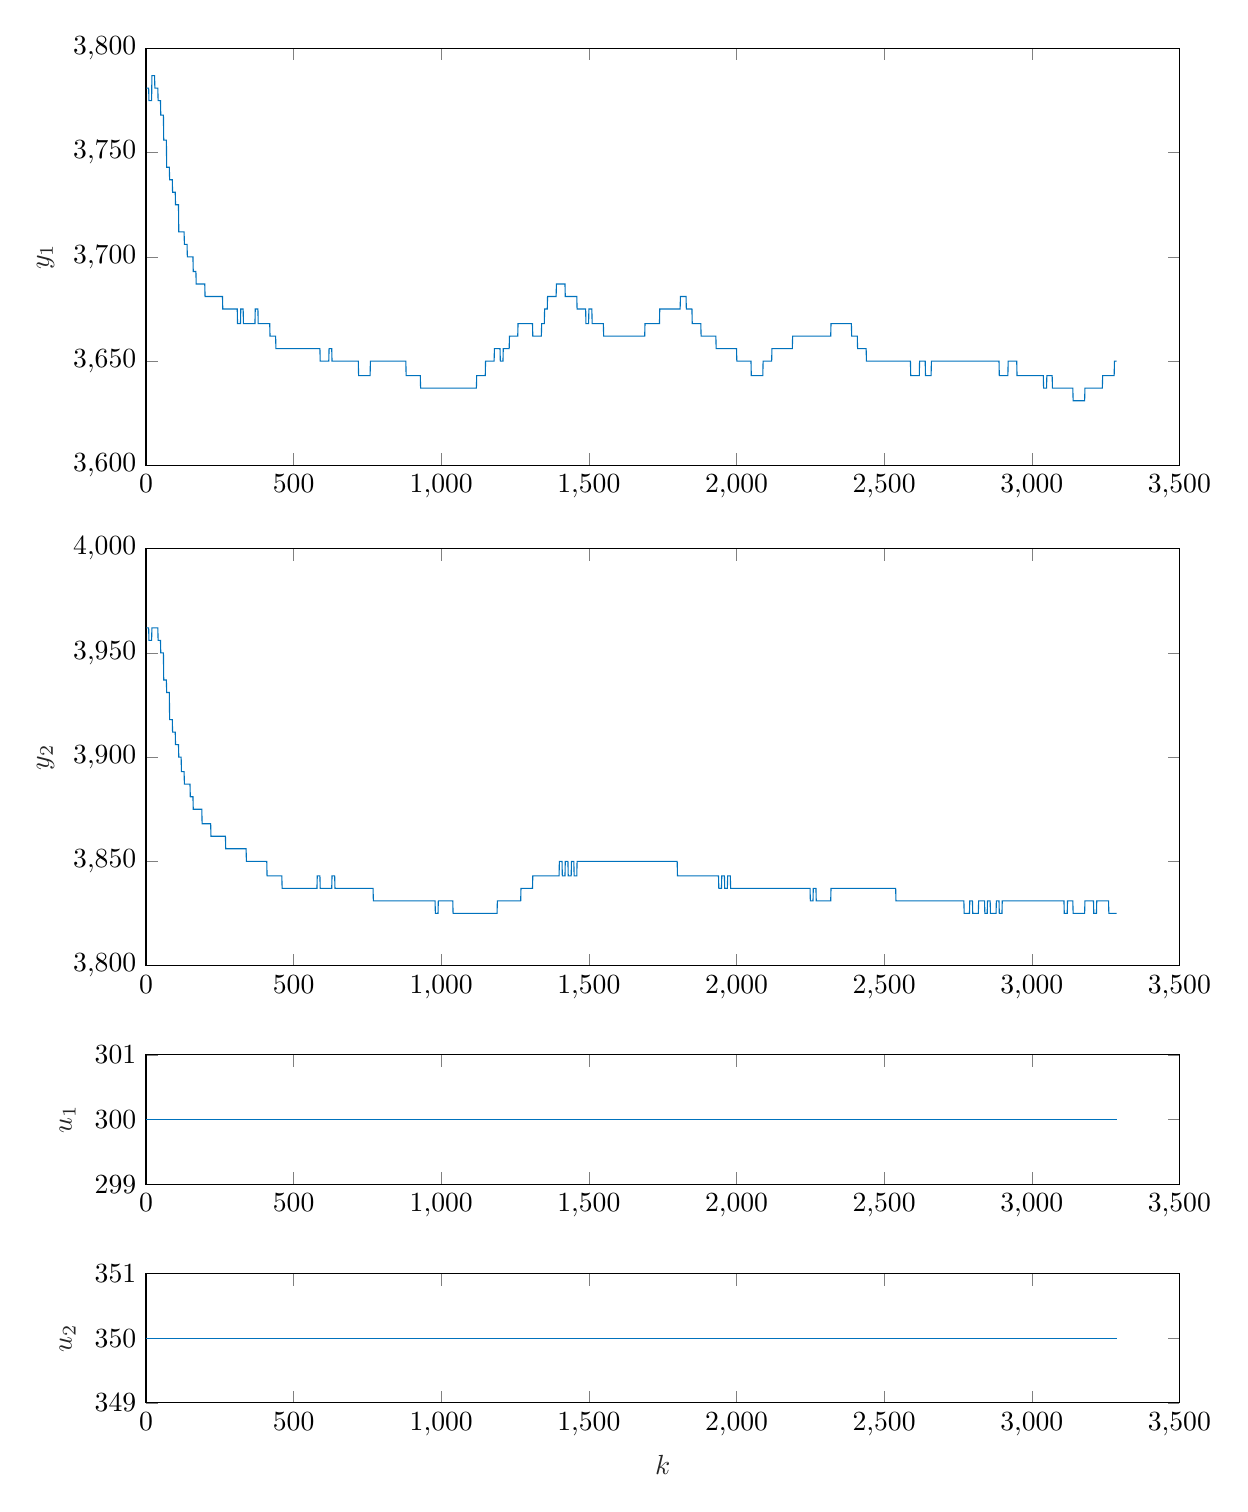
\begin{tikzpicture}

\begin{axis}[%
width=5.167in,
height=0.646in,
at={(0.646in,0.521in)},
scale only axis,
xmin=0,
xmax=3500,
xtick={0,500,1000,1500,2000,2500,3000,3500},
xlabel style={font=\color{white!15!black}},
xlabel={$k$},
ymin=349,
ymax=351,
ytick={349,350,351},
ylabel style={font=\color{white!15!black}},
ylabel={$u_2$},
axis background/.style={fill=white}
]
\addplot[const plot, color=mycolor1, forget plot] table[row sep=crcr] {%
1	350\\
2	350\\
3	350\\
4	350\\
5	350\\
6	350\\
7	350\\
8	350\\
9	350\\
10	350\\
11	350\\
12	350\\
13	350\\
14	350\\
15	350\\
16	350\\
17	350\\
18	350\\
19	350\\
20	350\\
21	350\\
22	350\\
23	350\\
24	350\\
25	350\\
26	350\\
27	350\\
28	350\\
29	350\\
30	350\\
31	350\\
32	350\\
33	350\\
34	350\\
35	350\\
36	350\\
37	350\\
38	350\\
39	350\\
40	350\\
41	350\\
42	350\\
43	350\\
44	350\\
45	350\\
46	350\\
47	350\\
48	350\\
49	350\\
50	350\\
51	350\\
52	350\\
53	350\\
54	350\\
55	350\\
56	350\\
57	350\\
58	350\\
59	350\\
60	350\\
61	350\\
62	350\\
63	350\\
64	350\\
65	350\\
66	350\\
67	350\\
68	350\\
69	350\\
70	350\\
71	350\\
72	350\\
73	350\\
74	350\\
75	350\\
76	350\\
77	350\\
78	350\\
79	350\\
80	350\\
81	350\\
82	350\\
83	350\\
84	350\\
85	350\\
86	350\\
87	350\\
88	350\\
89	350\\
90	350\\
91	350\\
92	350\\
93	350\\
94	350\\
95	350\\
96	350\\
97	350\\
98	350\\
99	350\\
100	350\\
101	350\\
102	350\\
103	350\\
104	350\\
105	350\\
106	350\\
107	350\\
108	350\\
109	350\\
110	350\\
111	350\\
112	350\\
113	350\\
114	350\\
115	350\\
116	350\\
117	350\\
118	350\\
119	350\\
120	350\\
121	350\\
122	350\\
123	350\\
124	350\\
125	350\\
126	350\\
127	350\\
128	350\\
129	350\\
130	350\\
131	350\\
132	350\\
133	350\\
134	350\\
135	350\\
136	350\\
137	350\\
138	350\\
139	350\\
140	350\\
141	350\\
142	350\\
143	350\\
144	350\\
145	350\\
146	350\\
147	350\\
148	350\\
149	350\\
150	350\\
151	350\\
152	350\\
153	350\\
154	350\\
155	350\\
156	350\\
157	350\\
158	350\\
159	350\\
160	350\\
161	350\\
162	350\\
163	350\\
164	350\\
165	350\\
166	350\\
167	350\\
168	350\\
169	350\\
170	350\\
171	350\\
172	350\\
173	350\\
174	350\\
175	350\\
176	350\\
177	350\\
178	350\\
179	350\\
180	350\\
181	350\\
182	350\\
183	350\\
184	350\\
185	350\\
186	350\\
187	350\\
188	350\\
189	350\\
190	350\\
191	350\\
192	350\\
193	350\\
194	350\\
195	350\\
196	350\\
197	350\\
198	350\\
199	350\\
200	350\\
201	350\\
202	350\\
203	350\\
204	350\\
205	350\\
206	350\\
207	350\\
208	350\\
209	350\\
210	350\\
211	350\\
212	350\\
213	350\\
214	350\\
215	350\\
216	350\\
217	350\\
218	350\\
219	350\\
220	350\\
221	350\\
222	350\\
223	350\\
224	350\\
225	350\\
226	350\\
227	350\\
228	350\\
229	350\\
230	350\\
231	350\\
232	350\\
233	350\\
234	350\\
235	350\\
236	350\\
237	350\\
238	350\\
239	350\\
240	350\\
241	350\\
242	350\\
243	350\\
244	350\\
245	350\\
246	350\\
247	350\\
248	350\\
249	350\\
250	350\\
251	350\\
252	350\\
253	350\\
254	350\\
255	350\\
256	350\\
257	350\\
258	350\\
259	350\\
260	350\\
261	350\\
262	350\\
263	350\\
264	350\\
265	350\\
266	350\\
267	350\\
268	350\\
269	350\\
270	350\\
271	350\\
272	350\\
273	350\\
274	350\\
275	350\\
276	350\\
277	350\\
278	350\\
279	350\\
280	350\\
281	350\\
282	350\\
283	350\\
284	350\\
285	350\\
286	350\\
287	350\\
288	350\\
289	350\\
290	350\\
291	350\\
292	350\\
293	350\\
294	350\\
295	350\\
296	350\\
297	350\\
298	350\\
299	350\\
300	350\\
301	350\\
302	350\\
303	350\\
304	350\\
305	350\\
306	350\\
307	350\\
308	350\\
309	350\\
310	350\\
311	350\\
312	350\\
313	350\\
314	350\\
315	350\\
316	350\\
317	350\\
318	350\\
319	350\\
320	350\\
321	350\\
322	350\\
323	350\\
324	350\\
325	350\\
326	350\\
327	350\\
328	350\\
329	350\\
330	350\\
331	350\\
332	350\\
333	350\\
334	350\\
335	350\\
336	350\\
337	350\\
338	350\\
339	350\\
340	350\\
341	350\\
342	350\\
343	350\\
344	350\\
345	350\\
346	350\\
347	350\\
348	350\\
349	350\\
350	350\\
351	350\\
352	350\\
353	350\\
354	350\\
355	350\\
356	350\\
357	350\\
358	350\\
359	350\\
360	350\\
361	350\\
362	350\\
363	350\\
364	350\\
365	350\\
366	350\\
367	350\\
368	350\\
369	350\\
370	350\\
371	350\\
372	350\\
373	350\\
374	350\\
375	350\\
376	350\\
377	350\\
378	350\\
379	350\\
380	350\\
381	350\\
382	350\\
383	350\\
384	350\\
385	350\\
386	350\\
387	350\\
388	350\\
389	350\\
390	350\\
391	350\\
392	350\\
393	350\\
394	350\\
395	350\\
396	350\\
397	350\\
398	350\\
399	350\\
400	350\\
401	350\\
402	350\\
403	350\\
404	350\\
405	350\\
406	350\\
407	350\\
408	350\\
409	350\\
410	350\\
411	350\\
412	350\\
413	350\\
414	350\\
415	350\\
416	350\\
417	350\\
418	350\\
419	350\\
420	350\\
421	350\\
422	350\\
423	350\\
424	350\\
425	350\\
426	350\\
427	350\\
428	350\\
429	350\\
430	350\\
431	350\\
432	350\\
433	350\\
434	350\\
435	350\\
436	350\\
437	350\\
438	350\\
439	350\\
440	350\\
441	350\\
442	350\\
443	350\\
444	350\\
445	350\\
446	350\\
447	350\\
448	350\\
449	350\\
450	350\\
451	350\\
452	350\\
453	350\\
454	350\\
455	350\\
456	350\\
457	350\\
458	350\\
459	350\\
460	350\\
461	350\\
462	350\\
463	350\\
464	350\\
465	350\\
466	350\\
467	350\\
468	350\\
469	350\\
470	350\\
471	350\\
472	350\\
473	350\\
474	350\\
475	350\\
476	350\\
477	350\\
478	350\\
479	350\\
480	350\\
481	350\\
482	350\\
483	350\\
484	350\\
485	350\\
486	350\\
487	350\\
488	350\\
489	350\\
490	350\\
491	350\\
492	350\\
493	350\\
494	350\\
495	350\\
496	350\\
497	350\\
498	350\\
499	350\\
500	350\\
501	350\\
502	350\\
503	350\\
504	350\\
505	350\\
506	350\\
507	350\\
508	350\\
509	350\\
510	350\\
511	350\\
512	350\\
513	350\\
514	350\\
515	350\\
516	350\\
517	350\\
518	350\\
519	350\\
520	350\\
521	350\\
522	350\\
523	350\\
524	350\\
525	350\\
526	350\\
527	350\\
528	350\\
529	350\\
530	350\\
531	350\\
532	350\\
533	350\\
534	350\\
535	350\\
536	350\\
537	350\\
538	350\\
539	350\\
540	350\\
541	350\\
542	350\\
543	350\\
544	350\\
545	350\\
546	350\\
547	350\\
548	350\\
549	350\\
550	350\\
551	350\\
552	350\\
553	350\\
554	350\\
555	350\\
556	350\\
557	350\\
558	350\\
559	350\\
560	350\\
561	350\\
562	350\\
563	350\\
564	350\\
565	350\\
566	350\\
567	350\\
568	350\\
569	350\\
570	350\\
571	350\\
572	350\\
573	350\\
574	350\\
575	350\\
576	350\\
577	350\\
578	350\\
579	350\\
580	350\\
581	350\\
582	350\\
583	350\\
584	350\\
585	350\\
586	350\\
587	350\\
588	350\\
589	350\\
590	350\\
591	350\\
592	350\\
593	350\\
594	350\\
595	350\\
596	350\\
597	350\\
598	350\\
599	350\\
600	350\\
601	350\\
602	350\\
603	350\\
604	350\\
605	350\\
606	350\\
607	350\\
608	350\\
609	350\\
610	350\\
611	350\\
612	350\\
613	350\\
614	350\\
615	350\\
616	350\\
617	350\\
618	350\\
619	350\\
620	350\\
621	350\\
622	350\\
623	350\\
624	350\\
625	350\\
626	350\\
627	350\\
628	350\\
629	350\\
630	350\\
631	350\\
632	350\\
633	350\\
634	350\\
635	350\\
636	350\\
637	350\\
638	350\\
639	350\\
640	350\\
641	350\\
642	350\\
643	350\\
644	350\\
645	350\\
646	350\\
647	350\\
648	350\\
649	350\\
650	350\\
651	350\\
652	350\\
653	350\\
654	350\\
655	350\\
656	350\\
657	350\\
658	350\\
659	350\\
660	350\\
661	350\\
662	350\\
663	350\\
664	350\\
665	350\\
666	350\\
667	350\\
668	350\\
669	350\\
670	350\\
671	350\\
672	350\\
673	350\\
674	350\\
675	350\\
676	350\\
677	350\\
678	350\\
679	350\\
680	350\\
681	350\\
682	350\\
683	350\\
684	350\\
685	350\\
686	350\\
687	350\\
688	350\\
689	350\\
690	350\\
691	350\\
692	350\\
693	350\\
694	350\\
695	350\\
696	350\\
697	350\\
698	350\\
699	350\\
700	350\\
701	350\\
702	350\\
703	350\\
704	350\\
705	350\\
706	350\\
707	350\\
708	350\\
709	350\\
710	350\\
711	350\\
712	350\\
713	350\\
714	350\\
715	350\\
716	350\\
717	350\\
718	350\\
719	350\\
720	350\\
721	350\\
722	350\\
723	350\\
724	350\\
725	350\\
726	350\\
727	350\\
728	350\\
729	350\\
730	350\\
731	350\\
732	350\\
733	350\\
734	350\\
735	350\\
736	350\\
737	350\\
738	350\\
739	350\\
740	350\\
741	350\\
742	350\\
743	350\\
744	350\\
745	350\\
746	350\\
747	350\\
748	350\\
749	350\\
750	350\\
751	350\\
752	350\\
753	350\\
754	350\\
755	350\\
756	350\\
757	350\\
758	350\\
759	350\\
760	350\\
761	350\\
762	350\\
763	350\\
764	350\\
765	350\\
766	350\\
767	350\\
768	350\\
769	350\\
770	350\\
771	350\\
772	350\\
773	350\\
774	350\\
775	350\\
776	350\\
777	350\\
778	350\\
779	350\\
780	350\\
781	350\\
782	350\\
783	350\\
784	350\\
785	350\\
786	350\\
787	350\\
788	350\\
789	350\\
790	350\\
791	350\\
792	350\\
793	350\\
794	350\\
795	350\\
796	350\\
797	350\\
798	350\\
799	350\\
800	350\\
801	350\\
802	350\\
803	350\\
804	350\\
805	350\\
806	350\\
807	350\\
808	350\\
809	350\\
810	350\\
811	350\\
812	350\\
813	350\\
814	350\\
815	350\\
816	350\\
817	350\\
818	350\\
819	350\\
820	350\\
821	350\\
822	350\\
823	350\\
824	350\\
825	350\\
826	350\\
827	350\\
828	350\\
829	350\\
830	350\\
831	350\\
832	350\\
833	350\\
834	350\\
835	350\\
836	350\\
837	350\\
838	350\\
839	350\\
840	350\\
841	350\\
842	350\\
843	350\\
844	350\\
845	350\\
846	350\\
847	350\\
848	350\\
849	350\\
850	350\\
851	350\\
852	350\\
853	350\\
854	350\\
855	350\\
856	350\\
857	350\\
858	350\\
859	350\\
860	350\\
861	350\\
862	350\\
863	350\\
864	350\\
865	350\\
866	350\\
867	350\\
868	350\\
869	350\\
870	350\\
871	350\\
872	350\\
873	350\\
874	350\\
875	350\\
876	350\\
877	350\\
878	350\\
879	350\\
880	350\\
881	350\\
882	350\\
883	350\\
884	350\\
885	350\\
886	350\\
887	350\\
888	350\\
889	350\\
890	350\\
891	350\\
892	350\\
893	350\\
894	350\\
895	350\\
896	350\\
897	350\\
898	350\\
899	350\\
900	350\\
901	350\\
902	350\\
903	350\\
904	350\\
905	350\\
906	350\\
907	350\\
908	350\\
909	350\\
910	350\\
911	350\\
912	350\\
913	350\\
914	350\\
915	350\\
916	350\\
917	350\\
918	350\\
919	350\\
920	350\\
921	350\\
922	350\\
923	350\\
924	350\\
925	350\\
926	350\\
927	350\\
928	350\\
929	350\\
930	350\\
931	350\\
932	350\\
933	350\\
934	350\\
935	350\\
936	350\\
937	350\\
938	350\\
939	350\\
940	350\\
941	350\\
942	350\\
943	350\\
944	350\\
945	350\\
946	350\\
947	350\\
948	350\\
949	350\\
950	350\\
951	350\\
952	350\\
953	350\\
954	350\\
955	350\\
956	350\\
957	350\\
958	350\\
959	350\\
960	350\\
961	350\\
962	350\\
963	350\\
964	350\\
965	350\\
966	350\\
967	350\\
968	350\\
969	350\\
970	350\\
971	350\\
972	350\\
973	350\\
974	350\\
975	350\\
976	350\\
977	350\\
978	350\\
979	350\\
980	350\\
981	350\\
982	350\\
983	350\\
984	350\\
985	350\\
986	350\\
987	350\\
988	350\\
989	350\\
990	350\\
991	350\\
992	350\\
993	350\\
994	350\\
995	350\\
996	350\\
997	350\\
998	350\\
999	350\\
1000	350\\
1001	350\\
1002	350\\
1003	350\\
1004	350\\
1005	350\\
1006	350\\
1007	350\\
1008	350\\
1009	350\\
1010	350\\
1011	350\\
1012	350\\
1013	350\\
1014	350\\
1015	350\\
1016	350\\
1017	350\\
1018	350\\
1019	350\\
1020	350\\
1021	350\\
1022	350\\
1023	350\\
1024	350\\
1025	350\\
1026	350\\
1027	350\\
1028	350\\
1029	350\\
1030	350\\
1031	350\\
1032	350\\
1033	350\\
1034	350\\
1035	350\\
1036	350\\
1037	350\\
1038	350\\
1039	350\\
1040	350\\
1041	350\\
1042	350\\
1043	350\\
1044	350\\
1045	350\\
1046	350\\
1047	350\\
1048	350\\
1049	350\\
1050	350\\
1051	350\\
1052	350\\
1053	350\\
1054	350\\
1055	350\\
1056	350\\
1057	350\\
1058	350\\
1059	350\\
1060	350\\
1061	350\\
1062	350\\
1063	350\\
1064	350\\
1065	350\\
1066	350\\
1067	350\\
1068	350\\
1069	350\\
1070	350\\
1071	350\\
1072	350\\
1073	350\\
1074	350\\
1075	350\\
1076	350\\
1077	350\\
1078	350\\
1079	350\\
1080	350\\
1081	350\\
1082	350\\
1083	350\\
1084	350\\
1085	350\\
1086	350\\
1087	350\\
1088	350\\
1089	350\\
1090	350\\
1091	350\\
1092	350\\
1093	350\\
1094	350\\
1095	350\\
1096	350\\
1097	350\\
1098	350\\
1099	350\\
1100	350\\
1101	350\\
1102	350\\
1103	350\\
1104	350\\
1105	350\\
1106	350\\
1107	350\\
1108	350\\
1109	350\\
1110	350\\
1111	350\\
1112	350\\
1113	350\\
1114	350\\
1115	350\\
1116	350\\
1117	350\\
1118	350\\
1119	350\\
1120	350\\
1121	350\\
1122	350\\
1123	350\\
1124	350\\
1125	350\\
1126	350\\
1127	350\\
1128	350\\
1129	350\\
1130	350\\
1131	350\\
1132	350\\
1133	350\\
1134	350\\
1135	350\\
1136	350\\
1137	350\\
1138	350\\
1139	350\\
1140	350\\
1141	350\\
1142	350\\
1143	350\\
1144	350\\
1145	350\\
1146	350\\
1147	350\\
1148	350\\
1149	350\\
1150	350\\
1151	350\\
1152	350\\
1153	350\\
1154	350\\
1155	350\\
1156	350\\
1157	350\\
1158	350\\
1159	350\\
1160	350\\
1161	350\\
1162	350\\
1163	350\\
1164	350\\
1165	350\\
1166	350\\
1167	350\\
1168	350\\
1169	350\\
1170	350\\
1171	350\\
1172	350\\
1173	350\\
1174	350\\
1175	350\\
1176	350\\
1177	350\\
1178	350\\
1179	350\\
1180	350\\
1181	350\\
1182	350\\
1183	350\\
1184	350\\
1185	350\\
1186	350\\
1187	350\\
1188	350\\
1189	350\\
1190	350\\
1191	350\\
1192	350\\
1193	350\\
1194	350\\
1195	350\\
1196	350\\
1197	350\\
1198	350\\
1199	350\\
1200	350\\
1201	350\\
1202	350\\
1203	350\\
1204	350\\
1205	350\\
1206	350\\
1207	350\\
1208	350\\
1209	350\\
1210	350\\
1211	350\\
1212	350\\
1213	350\\
1214	350\\
1215	350\\
1216	350\\
1217	350\\
1218	350\\
1219	350\\
1220	350\\
1221	350\\
1222	350\\
1223	350\\
1224	350\\
1225	350\\
1226	350\\
1227	350\\
1228	350\\
1229	350\\
1230	350\\
1231	350\\
1232	350\\
1233	350\\
1234	350\\
1235	350\\
1236	350\\
1237	350\\
1238	350\\
1239	350\\
1240	350\\
1241	350\\
1242	350\\
1243	350\\
1244	350\\
1245	350\\
1246	350\\
1247	350\\
1248	350\\
1249	350\\
1250	350\\
1251	350\\
1252	350\\
1253	350\\
1254	350\\
1255	350\\
1256	350\\
1257	350\\
1258	350\\
1259	350\\
1260	350\\
1261	350\\
1262	350\\
1263	350\\
1264	350\\
1265	350\\
1266	350\\
1267	350\\
1268	350\\
1269	350\\
1270	350\\
1271	350\\
1272	350\\
1273	350\\
1274	350\\
1275	350\\
1276	350\\
1277	350\\
1278	350\\
1279	350\\
1280	350\\
1281	350\\
1282	350\\
1283	350\\
1284	350\\
1285	350\\
1286	350\\
1287	350\\
1288	350\\
1289	350\\
1290	350\\
1291	350\\
1292	350\\
1293	350\\
1294	350\\
1295	350\\
1296	350\\
1297	350\\
1298	350\\
1299	350\\
1300	350\\
1301	350\\
1302	350\\
1303	350\\
1304	350\\
1305	350\\
1306	350\\
1307	350\\
1308	350\\
1309	350\\
1310	350\\
1311	350\\
1312	350\\
1313	350\\
1314	350\\
1315	350\\
1316	350\\
1317	350\\
1318	350\\
1319	350\\
1320	350\\
1321	350\\
1322	350\\
1323	350\\
1324	350\\
1325	350\\
1326	350\\
1327	350\\
1328	350\\
1329	350\\
1330	350\\
1331	350\\
1332	350\\
1333	350\\
1334	350\\
1335	350\\
1336	350\\
1337	350\\
1338	350\\
1339	350\\
1340	350\\
1341	350\\
1342	350\\
1343	350\\
1344	350\\
1345	350\\
1346	350\\
1347	350\\
1348	350\\
1349	350\\
1350	350\\
1351	350\\
1352	350\\
1353	350\\
1354	350\\
1355	350\\
1356	350\\
1357	350\\
1358	350\\
1359	350\\
1360	350\\
1361	350\\
1362	350\\
1363	350\\
1364	350\\
1365	350\\
1366	350\\
1367	350\\
1368	350\\
1369	350\\
1370	350\\
1371	350\\
1372	350\\
1373	350\\
1374	350\\
1375	350\\
1376	350\\
1377	350\\
1378	350\\
1379	350\\
1380	350\\
1381	350\\
1382	350\\
1383	350\\
1384	350\\
1385	350\\
1386	350\\
1387	350\\
1388	350\\
1389	350\\
1390	350\\
1391	350\\
1392	350\\
1393	350\\
1394	350\\
1395	350\\
1396	350\\
1397	350\\
1398	350\\
1399	350\\
1400	350\\
1401	350\\
1402	350\\
1403	350\\
1404	350\\
1405	350\\
1406	350\\
1407	350\\
1408	350\\
1409	350\\
1410	350\\
1411	350\\
1412	350\\
1413	350\\
1414	350\\
1415	350\\
1416	350\\
1417	350\\
1418	350\\
1419	350\\
1420	350\\
1421	350\\
1422	350\\
1423	350\\
1424	350\\
1425	350\\
1426	350\\
1427	350\\
1428	350\\
1429	350\\
1430	350\\
1431	350\\
1432	350\\
1433	350\\
1434	350\\
1435	350\\
1436	350\\
1437	350\\
1438	350\\
1439	350\\
1440	350\\
1441	350\\
1442	350\\
1443	350\\
1444	350\\
1445	350\\
1446	350\\
1447	350\\
1448	350\\
1449	350\\
1450	350\\
1451	350\\
1452	350\\
1453	350\\
1454	350\\
1455	350\\
1456	350\\
1457	350\\
1458	350\\
1459	350\\
1460	350\\
1461	350\\
1462	350\\
1463	350\\
1464	350\\
1465	350\\
1466	350\\
1467	350\\
1468	350\\
1469	350\\
1470	350\\
1471	350\\
1472	350\\
1473	350\\
1474	350\\
1475	350\\
1476	350\\
1477	350\\
1478	350\\
1479	350\\
1480	350\\
1481	350\\
1482	350\\
1483	350\\
1484	350\\
1485	350\\
1486	350\\
1487	350\\
1488	350\\
1489	350\\
1490	350\\
1491	350\\
1492	350\\
1493	350\\
1494	350\\
1495	350\\
1496	350\\
1497	350\\
1498	350\\
1499	350\\
1500	350\\
1501	350\\
1502	350\\
1503	350\\
1504	350\\
1505	350\\
1506	350\\
1507	350\\
1508	350\\
1509	350\\
1510	350\\
1511	350\\
1512	350\\
1513	350\\
1514	350\\
1515	350\\
1516	350\\
1517	350\\
1518	350\\
1519	350\\
1520	350\\
1521	350\\
1522	350\\
1523	350\\
1524	350\\
1525	350\\
1526	350\\
1527	350\\
1528	350\\
1529	350\\
1530	350\\
1531	350\\
1532	350\\
1533	350\\
1534	350\\
1535	350\\
1536	350\\
1537	350\\
1538	350\\
1539	350\\
1540	350\\
1541	350\\
1542	350\\
1543	350\\
1544	350\\
1545	350\\
1546	350\\
1547	350\\
1548	350\\
1549	350\\
1550	350\\
1551	350\\
1552	350\\
1553	350\\
1554	350\\
1555	350\\
1556	350\\
1557	350\\
1558	350\\
1559	350\\
1560	350\\
1561	350\\
1562	350\\
1563	350\\
1564	350\\
1565	350\\
1566	350\\
1567	350\\
1568	350\\
1569	350\\
1570	350\\
1571	350\\
1572	350\\
1573	350\\
1574	350\\
1575	350\\
1576	350\\
1577	350\\
1578	350\\
1579	350\\
1580	350\\
1581	350\\
1582	350\\
1583	350\\
1584	350\\
1585	350\\
1586	350\\
1587	350\\
1588	350\\
1589	350\\
1590	350\\
1591	350\\
1592	350\\
1593	350\\
1594	350\\
1595	350\\
1596	350\\
1597	350\\
1598	350\\
1599	350\\
1600	350\\
1601	350\\
1602	350\\
1603	350\\
1604	350\\
1605	350\\
1606	350\\
1607	350\\
1608	350\\
1609	350\\
1610	350\\
1611	350\\
1612	350\\
1613	350\\
1614	350\\
1615	350\\
1616	350\\
1617	350\\
1618	350\\
1619	350\\
1620	350\\
1621	350\\
1622	350\\
1623	350\\
1624	350\\
1625	350\\
1626	350\\
1627	350\\
1628	350\\
1629	350\\
1630	350\\
1631	350\\
1632	350\\
1633	350\\
1634	350\\
1635	350\\
1636	350\\
1637	350\\
1638	350\\
1639	350\\
1640	350\\
1641	350\\
1642	350\\
1643	350\\
1644	350\\
1645	350\\
1646	350\\
1647	350\\
1648	350\\
1649	350\\
1650	350\\
1651	350\\
1652	350\\
1653	350\\
1654	350\\
1655	350\\
1656	350\\
1657	350\\
1658	350\\
1659	350\\
1660	350\\
1661	350\\
1662	350\\
1663	350\\
1664	350\\
1665	350\\
1666	350\\
1667	350\\
1668	350\\
1669	350\\
1670	350\\
1671	350\\
1672	350\\
1673	350\\
1674	350\\
1675	350\\
1676	350\\
1677	350\\
1678	350\\
1679	350\\
1680	350\\
1681	350\\
1682	350\\
1683	350\\
1684	350\\
1685	350\\
1686	350\\
1687	350\\
1688	350\\
1689	350\\
1690	350\\
1691	350\\
1692	350\\
1693	350\\
1694	350\\
1695	350\\
1696	350\\
1697	350\\
1698	350\\
1699	350\\
1700	350\\
1701	350\\
1702	350\\
1703	350\\
1704	350\\
1705	350\\
1706	350\\
1707	350\\
1708	350\\
1709	350\\
1710	350\\
1711	350\\
1712	350\\
1713	350\\
1714	350\\
1715	350\\
1716	350\\
1717	350\\
1718	350\\
1719	350\\
1720	350\\
1721	350\\
1722	350\\
1723	350\\
1724	350\\
1725	350\\
1726	350\\
1727	350\\
1728	350\\
1729	350\\
1730	350\\
1731	350\\
1732	350\\
1733	350\\
1734	350\\
1735	350\\
1736	350\\
1737	350\\
1738	350\\
1739	350\\
1740	350\\
1741	350\\
1742	350\\
1743	350\\
1744	350\\
1745	350\\
1746	350\\
1747	350\\
1748	350\\
1749	350\\
1750	350\\
1751	350\\
1752	350\\
1753	350\\
1754	350\\
1755	350\\
1756	350\\
1757	350\\
1758	350\\
1759	350\\
1760	350\\
1761	350\\
1762	350\\
1763	350\\
1764	350\\
1765	350\\
1766	350\\
1767	350\\
1768	350\\
1769	350\\
1770	350\\
1771	350\\
1772	350\\
1773	350\\
1774	350\\
1775	350\\
1776	350\\
1777	350\\
1778	350\\
1779	350\\
1780	350\\
1781	350\\
1782	350\\
1783	350\\
1784	350\\
1785	350\\
1786	350\\
1787	350\\
1788	350\\
1789	350\\
1790	350\\
1791	350\\
1792	350\\
1793	350\\
1794	350\\
1795	350\\
1796	350\\
1797	350\\
1798	350\\
1799	350\\
1800	350\\
1801	350\\
1802	350\\
1803	350\\
1804	350\\
1805	350\\
1806	350\\
1807	350\\
1808	350\\
1809	350\\
1810	350\\
1811	350\\
1812	350\\
1813	350\\
1814	350\\
1815	350\\
1816	350\\
1817	350\\
1818	350\\
1819	350\\
1820	350\\
1821	350\\
1822	350\\
1823	350\\
1824	350\\
1825	350\\
1826	350\\
1827	350\\
1828	350\\
1829	350\\
1830	350\\
1831	350\\
1832	350\\
1833	350\\
1834	350\\
1835	350\\
1836	350\\
1837	350\\
1838	350\\
1839	350\\
1840	350\\
1841	350\\
1842	350\\
1843	350\\
1844	350\\
1845	350\\
1846	350\\
1847	350\\
1848	350\\
1849	350\\
1850	350\\
1851	350\\
1852	350\\
1853	350\\
1854	350\\
1855	350\\
1856	350\\
1857	350\\
1858	350\\
1859	350\\
1860	350\\
1861	350\\
1862	350\\
1863	350\\
1864	350\\
1865	350\\
1866	350\\
1867	350\\
1868	350\\
1869	350\\
1870	350\\
1871	350\\
1872	350\\
1873	350\\
1874	350\\
1875	350\\
1876	350\\
1877	350\\
1878	350\\
1879	350\\
1880	350\\
1881	350\\
1882	350\\
1883	350\\
1884	350\\
1885	350\\
1886	350\\
1887	350\\
1888	350\\
1889	350\\
1890	350\\
1891	350\\
1892	350\\
1893	350\\
1894	350\\
1895	350\\
1896	350\\
1897	350\\
1898	350\\
1899	350\\
1900	350\\
1901	350\\
1902	350\\
1903	350\\
1904	350\\
1905	350\\
1906	350\\
1907	350\\
1908	350\\
1909	350\\
1910	350\\
1911	350\\
1912	350\\
1913	350\\
1914	350\\
1915	350\\
1916	350\\
1917	350\\
1918	350\\
1919	350\\
1920	350\\
1921	350\\
1922	350\\
1923	350\\
1924	350\\
1925	350\\
1926	350\\
1927	350\\
1928	350\\
1929	350\\
1930	350\\
1931	350\\
1932	350\\
1933	350\\
1934	350\\
1935	350\\
1936	350\\
1937	350\\
1938	350\\
1939	350\\
1940	350\\
1941	350\\
1942	350\\
1943	350\\
1944	350\\
1945	350\\
1946	350\\
1947	350\\
1948	350\\
1949	350\\
1950	350\\
1951	350\\
1952	350\\
1953	350\\
1954	350\\
1955	350\\
1956	350\\
1957	350\\
1958	350\\
1959	350\\
1960	350\\
1961	350\\
1962	350\\
1963	350\\
1964	350\\
1965	350\\
1966	350\\
1967	350\\
1968	350\\
1969	350\\
1970	350\\
1971	350\\
1972	350\\
1973	350\\
1974	350\\
1975	350\\
1976	350\\
1977	350\\
1978	350\\
1979	350\\
1980	350\\
1981	350\\
1982	350\\
1983	350\\
1984	350\\
1985	350\\
1986	350\\
1987	350\\
1988	350\\
1989	350\\
1990	350\\
1991	350\\
1992	350\\
1993	350\\
1994	350\\
1995	350\\
1996	350\\
1997	350\\
1998	350\\
1999	350\\
2000	350\\
2001	350\\
2002	350\\
2003	350\\
2004	350\\
2005	350\\
2006	350\\
2007	350\\
2008	350\\
2009	350\\
2010	350\\
2011	350\\
2012	350\\
2013	350\\
2014	350\\
2015	350\\
2016	350\\
2017	350\\
2018	350\\
2019	350\\
2020	350\\
2021	350\\
2022	350\\
2023	350\\
2024	350\\
2025	350\\
2026	350\\
2027	350\\
2028	350\\
2029	350\\
2030	350\\
2031	350\\
2032	350\\
2033	350\\
2034	350\\
2035	350\\
2036	350\\
2037	350\\
2038	350\\
2039	350\\
2040	350\\
2041	350\\
2042	350\\
2043	350\\
2044	350\\
2045	350\\
2046	350\\
2047	350\\
2048	350\\
2049	350\\
2050	350\\
2051	350\\
2052	350\\
2053	350\\
2054	350\\
2055	350\\
2056	350\\
2057	350\\
2058	350\\
2059	350\\
2060	350\\
2061	350\\
2062	350\\
2063	350\\
2064	350\\
2065	350\\
2066	350\\
2067	350\\
2068	350\\
2069	350\\
2070	350\\
2071	350\\
2072	350\\
2073	350\\
2074	350\\
2075	350\\
2076	350\\
2077	350\\
2078	350\\
2079	350\\
2080	350\\
2081	350\\
2082	350\\
2083	350\\
2084	350\\
2085	350\\
2086	350\\
2087	350\\
2088	350\\
2089	350\\
2090	350\\
2091	350\\
2092	350\\
2093	350\\
2094	350\\
2095	350\\
2096	350\\
2097	350\\
2098	350\\
2099	350\\
2100	350\\
2101	350\\
2102	350\\
2103	350\\
2104	350\\
2105	350\\
2106	350\\
2107	350\\
2108	350\\
2109	350\\
2110	350\\
2111	350\\
2112	350\\
2113	350\\
2114	350\\
2115	350\\
2116	350\\
2117	350\\
2118	350\\
2119	350\\
2120	350\\
2121	350\\
2122	350\\
2123	350\\
2124	350\\
2125	350\\
2126	350\\
2127	350\\
2128	350\\
2129	350\\
2130	350\\
2131	350\\
2132	350\\
2133	350\\
2134	350\\
2135	350\\
2136	350\\
2137	350\\
2138	350\\
2139	350\\
2140	350\\
2141	350\\
2142	350\\
2143	350\\
2144	350\\
2145	350\\
2146	350\\
2147	350\\
2148	350\\
2149	350\\
2150	350\\
2151	350\\
2152	350\\
2153	350\\
2154	350\\
2155	350\\
2156	350\\
2157	350\\
2158	350\\
2159	350\\
2160	350\\
2161	350\\
2162	350\\
2163	350\\
2164	350\\
2165	350\\
2166	350\\
2167	350\\
2168	350\\
2169	350\\
2170	350\\
2171	350\\
2172	350\\
2173	350\\
2174	350\\
2175	350\\
2176	350\\
2177	350\\
2178	350\\
2179	350\\
2180	350\\
2181	350\\
2182	350\\
2183	350\\
2184	350\\
2185	350\\
2186	350\\
2187	350\\
2188	350\\
2189	350\\
2190	350\\
2191	350\\
2192	350\\
2193	350\\
2194	350\\
2195	350\\
2196	350\\
2197	350\\
2198	350\\
2199	350\\
2200	350\\
2201	350\\
2202	350\\
2203	350\\
2204	350\\
2205	350\\
2206	350\\
2207	350\\
2208	350\\
2209	350\\
2210	350\\
2211	350\\
2212	350\\
2213	350\\
2214	350\\
2215	350\\
2216	350\\
2217	350\\
2218	350\\
2219	350\\
2220	350\\
2221	350\\
2222	350\\
2223	350\\
2224	350\\
2225	350\\
2226	350\\
2227	350\\
2228	350\\
2229	350\\
2230	350\\
2231	350\\
2232	350\\
2233	350\\
2234	350\\
2235	350\\
2236	350\\
2237	350\\
2238	350\\
2239	350\\
2240	350\\
2241	350\\
2242	350\\
2243	350\\
2244	350\\
2245	350\\
2246	350\\
2247	350\\
2248	350\\
2249	350\\
2250	350\\
2251	350\\
2252	350\\
2253	350\\
2254	350\\
2255	350\\
2256	350\\
2257	350\\
2258	350\\
2259	350\\
2260	350\\
2261	350\\
2262	350\\
2263	350\\
2264	350\\
2265	350\\
2266	350\\
2267	350\\
2268	350\\
2269	350\\
2270	350\\
2271	350\\
2272	350\\
2273	350\\
2274	350\\
2275	350\\
2276	350\\
2277	350\\
2278	350\\
2279	350\\
2280	350\\
2281	350\\
2282	350\\
2283	350\\
2284	350\\
2285	350\\
2286	350\\
2287	350\\
2288	350\\
2289	350\\
2290	350\\
2291	350\\
2292	350\\
2293	350\\
2294	350\\
2295	350\\
2296	350\\
2297	350\\
2298	350\\
2299	350\\
2300	350\\
2301	350\\
2302	350\\
2303	350\\
2304	350\\
2305	350\\
2306	350\\
2307	350\\
2308	350\\
2309	350\\
2310	350\\
2311	350\\
2312	350\\
2313	350\\
2314	350\\
2315	350\\
2316	350\\
2317	350\\
2318	350\\
2319	350\\
2320	350\\
2321	350\\
2322	350\\
2323	350\\
2324	350\\
2325	350\\
2326	350\\
2327	350\\
2328	350\\
2329	350\\
2330	350\\
2331	350\\
2332	350\\
2333	350\\
2334	350\\
2335	350\\
2336	350\\
2337	350\\
2338	350\\
2339	350\\
2340	350\\
2341	350\\
2342	350\\
2343	350\\
2344	350\\
2345	350\\
2346	350\\
2347	350\\
2348	350\\
2349	350\\
2350	350\\
2351	350\\
2352	350\\
2353	350\\
2354	350\\
2355	350\\
2356	350\\
2357	350\\
2358	350\\
2359	350\\
2360	350\\
2361	350\\
2362	350\\
2363	350\\
2364	350\\
2365	350\\
2366	350\\
2367	350\\
2368	350\\
2369	350\\
2370	350\\
2371	350\\
2372	350\\
2373	350\\
2374	350\\
2375	350\\
2376	350\\
2377	350\\
2378	350\\
2379	350\\
2380	350\\
2381	350\\
2382	350\\
2383	350\\
2384	350\\
2385	350\\
2386	350\\
2387	350\\
2388	350\\
2389	350\\
2390	350\\
2391	350\\
2392	350\\
2393	350\\
2394	350\\
2395	350\\
2396	350\\
2397	350\\
2398	350\\
2399	350\\
2400	350\\
2401	350\\
2402	350\\
2403	350\\
2404	350\\
2405	350\\
2406	350\\
2407	350\\
2408	350\\
2409	350\\
2410	350\\
2411	350\\
2412	350\\
2413	350\\
2414	350\\
2415	350\\
2416	350\\
2417	350\\
2418	350\\
2419	350\\
2420	350\\
2421	350\\
2422	350\\
2423	350\\
2424	350\\
2425	350\\
2426	350\\
2427	350\\
2428	350\\
2429	350\\
2430	350\\
2431	350\\
2432	350\\
2433	350\\
2434	350\\
2435	350\\
2436	350\\
2437	350\\
2438	350\\
2439	350\\
2440	350\\
2441	350\\
2442	350\\
2443	350\\
2444	350\\
2445	350\\
2446	350\\
2447	350\\
2448	350\\
2449	350\\
2450	350\\
2451	350\\
2452	350\\
2453	350\\
2454	350\\
2455	350\\
2456	350\\
2457	350\\
2458	350\\
2459	350\\
2460	350\\
2461	350\\
2462	350\\
2463	350\\
2464	350\\
2465	350\\
2466	350\\
2467	350\\
2468	350\\
2469	350\\
2470	350\\
2471	350\\
2472	350\\
2473	350\\
2474	350\\
2475	350\\
2476	350\\
2477	350\\
2478	350\\
2479	350\\
2480	350\\
2481	350\\
2482	350\\
2483	350\\
2484	350\\
2485	350\\
2486	350\\
2487	350\\
2488	350\\
2489	350\\
2490	350\\
2491	350\\
2492	350\\
2493	350\\
2494	350\\
2495	350\\
2496	350\\
2497	350\\
2498	350\\
2499	350\\
2500	350\\
2501	350\\
2502	350\\
2503	350\\
2504	350\\
2505	350\\
2506	350\\
2507	350\\
2508	350\\
2509	350\\
2510	350\\
2511	350\\
2512	350\\
2513	350\\
2514	350\\
2515	350\\
2516	350\\
2517	350\\
2518	350\\
2519	350\\
2520	350\\
2521	350\\
2522	350\\
2523	350\\
2524	350\\
2525	350\\
2526	350\\
2527	350\\
2528	350\\
2529	350\\
2530	350\\
2531	350\\
2532	350\\
2533	350\\
2534	350\\
2535	350\\
2536	350\\
2537	350\\
2538	350\\
2539	350\\
2540	350\\
2541	350\\
2542	350\\
2543	350\\
2544	350\\
2545	350\\
2546	350\\
2547	350\\
2548	350\\
2549	350\\
2550	350\\
2551	350\\
2552	350\\
2553	350\\
2554	350\\
2555	350\\
2556	350\\
2557	350\\
2558	350\\
2559	350\\
2560	350\\
2561	350\\
2562	350\\
2563	350\\
2564	350\\
2565	350\\
2566	350\\
2567	350\\
2568	350\\
2569	350\\
2570	350\\
2571	350\\
2572	350\\
2573	350\\
2574	350\\
2575	350\\
2576	350\\
2577	350\\
2578	350\\
2579	350\\
2580	350\\
2581	350\\
2582	350\\
2583	350\\
2584	350\\
2585	350\\
2586	350\\
2587	350\\
2588	350\\
2589	350\\
2590	350\\
2591	350\\
2592	350\\
2593	350\\
2594	350\\
2595	350\\
2596	350\\
2597	350\\
2598	350\\
2599	350\\
2600	350\\
2601	350\\
2602	350\\
2603	350\\
2604	350\\
2605	350\\
2606	350\\
2607	350\\
2608	350\\
2609	350\\
2610	350\\
2611	350\\
2612	350\\
2613	350\\
2614	350\\
2615	350\\
2616	350\\
2617	350\\
2618	350\\
2619	350\\
2620	350\\
2621	350\\
2622	350\\
2623	350\\
2624	350\\
2625	350\\
2626	350\\
2627	350\\
2628	350\\
2629	350\\
2630	350\\
2631	350\\
2632	350\\
2633	350\\
2634	350\\
2635	350\\
2636	350\\
2637	350\\
2638	350\\
2639	350\\
2640	350\\
2641	350\\
2642	350\\
2643	350\\
2644	350\\
2645	350\\
2646	350\\
2647	350\\
2648	350\\
2649	350\\
2650	350\\
2651	350\\
2652	350\\
2653	350\\
2654	350\\
2655	350\\
2656	350\\
2657	350\\
2658	350\\
2659	350\\
2660	350\\
2661	350\\
2662	350\\
2663	350\\
2664	350\\
2665	350\\
2666	350\\
2667	350\\
2668	350\\
2669	350\\
2670	350\\
2671	350\\
2672	350\\
2673	350\\
2674	350\\
2675	350\\
2676	350\\
2677	350\\
2678	350\\
2679	350\\
2680	350\\
2681	350\\
2682	350\\
2683	350\\
2684	350\\
2685	350\\
2686	350\\
2687	350\\
2688	350\\
2689	350\\
2690	350\\
2691	350\\
2692	350\\
2693	350\\
2694	350\\
2695	350\\
2696	350\\
2697	350\\
2698	350\\
2699	350\\
2700	350\\
2701	350\\
2702	350\\
2703	350\\
2704	350\\
2705	350\\
2706	350\\
2707	350\\
2708	350\\
2709	350\\
2710	350\\
2711	350\\
2712	350\\
2713	350\\
2714	350\\
2715	350\\
2716	350\\
2717	350\\
2718	350\\
2719	350\\
2720	350\\
2721	350\\
2722	350\\
2723	350\\
2724	350\\
2725	350\\
2726	350\\
2727	350\\
2728	350\\
2729	350\\
2730	350\\
2731	350\\
2732	350\\
2733	350\\
2734	350\\
2735	350\\
2736	350\\
2737	350\\
2738	350\\
2739	350\\
2740	350\\
2741	350\\
2742	350\\
2743	350\\
2744	350\\
2745	350\\
2746	350\\
2747	350\\
2748	350\\
2749	350\\
2750	350\\
2751	350\\
2752	350\\
2753	350\\
2754	350\\
2755	350\\
2756	350\\
2757	350\\
2758	350\\
2759	350\\
2760	350\\
2761	350\\
2762	350\\
2763	350\\
2764	350\\
2765	350\\
2766	350\\
2767	350\\
2768	350\\
2769	350\\
2770	350\\
2771	350\\
2772	350\\
2773	350\\
2774	350\\
2775	350\\
2776	350\\
2777	350\\
2778	350\\
2779	350\\
2780	350\\
2781	350\\
2782	350\\
2783	350\\
2784	350\\
2785	350\\
2786	350\\
2787	350\\
2788	350\\
2789	350\\
2790	350\\
2791	350\\
2792	350\\
2793	350\\
2794	350\\
2795	350\\
2796	350\\
2797	350\\
2798	350\\
2799	350\\
2800	350\\
2801	350\\
2802	350\\
2803	350\\
2804	350\\
2805	350\\
2806	350\\
2807	350\\
2808	350\\
2809	350\\
2810	350\\
2811	350\\
2812	350\\
2813	350\\
2814	350\\
2815	350\\
2816	350\\
2817	350\\
2818	350\\
2819	350\\
2820	350\\
2821	350\\
2822	350\\
2823	350\\
2824	350\\
2825	350\\
2826	350\\
2827	350\\
2828	350\\
2829	350\\
2830	350\\
2831	350\\
2832	350\\
2833	350\\
2834	350\\
2835	350\\
2836	350\\
2837	350\\
2838	350\\
2839	350\\
2840	350\\
2841	350\\
2842	350\\
2843	350\\
2844	350\\
2845	350\\
2846	350\\
2847	350\\
2848	350\\
2849	350\\
2850	350\\
2851	350\\
2852	350\\
2853	350\\
2854	350\\
2855	350\\
2856	350\\
2857	350\\
2858	350\\
2859	350\\
2860	350\\
2861	350\\
2862	350\\
2863	350\\
2864	350\\
2865	350\\
2866	350\\
2867	350\\
2868	350\\
2869	350\\
2870	350\\
2871	350\\
2872	350\\
2873	350\\
2874	350\\
2875	350\\
2876	350\\
2877	350\\
2878	350\\
2879	350\\
2880	350\\
2881	350\\
2882	350\\
2883	350\\
2884	350\\
2885	350\\
2886	350\\
2887	350\\
2888	350\\
2889	350\\
2890	350\\
2891	350\\
2892	350\\
2893	350\\
2894	350\\
2895	350\\
2896	350\\
2897	350\\
2898	350\\
2899	350\\
2900	350\\
2901	350\\
2902	350\\
2903	350\\
2904	350\\
2905	350\\
2906	350\\
2907	350\\
2908	350\\
2909	350\\
2910	350\\
2911	350\\
2912	350\\
2913	350\\
2914	350\\
2915	350\\
2916	350\\
2917	350\\
2918	350\\
2919	350\\
2920	350\\
2921	350\\
2922	350\\
2923	350\\
2924	350\\
2925	350\\
2926	350\\
2927	350\\
2928	350\\
2929	350\\
2930	350\\
2931	350\\
2932	350\\
2933	350\\
2934	350\\
2935	350\\
2936	350\\
2937	350\\
2938	350\\
2939	350\\
2940	350\\
2941	350\\
2942	350\\
2943	350\\
2944	350\\
2945	350\\
2946	350\\
2947	350\\
2948	350\\
2949	350\\
2950	350\\
2951	350\\
2952	350\\
2953	350\\
2954	350\\
2955	350\\
2956	350\\
2957	350\\
2958	350\\
2959	350\\
2960	350\\
2961	350\\
2962	350\\
2963	350\\
2964	350\\
2965	350\\
2966	350\\
2967	350\\
2968	350\\
2969	350\\
2970	350\\
2971	350\\
2972	350\\
2973	350\\
2974	350\\
2975	350\\
2976	350\\
2977	350\\
2978	350\\
2979	350\\
2980	350\\
2981	350\\
2982	350\\
2983	350\\
2984	350\\
2985	350\\
2986	350\\
2987	350\\
2988	350\\
2989	350\\
2990	350\\
2991	350\\
2992	350\\
2993	350\\
2994	350\\
2995	350\\
2996	350\\
2997	350\\
2998	350\\
2999	350\\
3000	350\\
3001	350\\
3002	350\\
3003	350\\
3004	350\\
3005	350\\
3006	350\\
3007	350\\
3008	350\\
3009	350\\
3010	350\\
3011	350\\
3012	350\\
3013	350\\
3014	350\\
3015	350\\
3016	350\\
3017	350\\
3018	350\\
3019	350\\
3020	350\\
3021	350\\
3022	350\\
3023	350\\
3024	350\\
3025	350\\
3026	350\\
3027	350\\
3028	350\\
3029	350\\
3030	350\\
3031	350\\
3032	350\\
3033	350\\
3034	350\\
3035	350\\
3036	350\\
3037	350\\
3038	350\\
3039	350\\
3040	350\\
3041	350\\
3042	350\\
3043	350\\
3044	350\\
3045	350\\
3046	350\\
3047	350\\
3048	350\\
3049	350\\
3050	350\\
3051	350\\
3052	350\\
3053	350\\
3054	350\\
3055	350\\
3056	350\\
3057	350\\
3058	350\\
3059	350\\
3060	350\\
3061	350\\
3062	350\\
3063	350\\
3064	350\\
3065	350\\
3066	350\\
3067	350\\
3068	350\\
3069	350\\
3070	350\\
3071	350\\
3072	350\\
3073	350\\
3074	350\\
3075	350\\
3076	350\\
3077	350\\
3078	350\\
3079	350\\
3080	350\\
3081	350\\
3082	350\\
3083	350\\
3084	350\\
3085	350\\
3086	350\\
3087	350\\
3088	350\\
3089	350\\
3090	350\\
3091	350\\
3092	350\\
3093	350\\
3094	350\\
3095	350\\
3096	350\\
3097	350\\
3098	350\\
3099	350\\
3100	350\\
3101	350\\
3102	350\\
3103	350\\
3104	350\\
3105	350\\
3106	350\\
3107	350\\
3108	350\\
3109	350\\
3110	350\\
3111	350\\
3112	350\\
3113	350\\
3114	350\\
3115	350\\
3116	350\\
3117	350\\
3118	350\\
3119	350\\
3120	350\\
3121	350\\
3122	350\\
3123	350\\
3124	350\\
3125	350\\
3126	350\\
3127	350\\
3128	350\\
3129	350\\
3130	350\\
3131	350\\
3132	350\\
3133	350\\
3134	350\\
3135	350\\
3136	350\\
3137	350\\
3138	350\\
3139	350\\
3140	350\\
3141	350\\
3142	350\\
3143	350\\
3144	350\\
3145	350\\
3146	350\\
3147	350\\
3148	350\\
3149	350\\
3150	350\\
3151	350\\
3152	350\\
3153	350\\
3154	350\\
3155	350\\
3156	350\\
3157	350\\
3158	350\\
3159	350\\
3160	350\\
3161	350\\
3162	350\\
3163	350\\
3164	350\\
3165	350\\
3166	350\\
3167	350\\
3168	350\\
3169	350\\
3170	350\\
3171	350\\
3172	350\\
3173	350\\
3174	350\\
3175	350\\
3176	350\\
3177	350\\
3178	350\\
3179	350\\
3180	350\\
3181	350\\
3182	350\\
3183	350\\
3184	350\\
3185	350\\
3186	350\\
3187	350\\
3188	350\\
3189	350\\
3190	350\\
3191	350\\
3192	350\\
3193	350\\
3194	350\\
3195	350\\
3196	350\\
3197	350\\
3198	350\\
3199	350\\
3200	350\\
3201	350\\
3202	350\\
3203	350\\
3204	350\\
3205	350\\
3206	350\\
3207	350\\
3208	350\\
3209	350\\
3210	350\\
3211	350\\
3212	350\\
3213	350\\
3214	350\\
3215	350\\
3216	350\\
3217	350\\
3218	350\\
3219	350\\
3220	350\\
3221	350\\
3222	350\\
3223	350\\
3224	350\\
3225	350\\
3226	350\\
3227	350\\
3228	350\\
3229	350\\
3230	350\\
3231	350\\
3232	350\\
3233	350\\
3234	350\\
3235	350\\
3236	350\\
3237	350\\
3238	350\\
3239	350\\
3240	350\\
3241	350\\
3242	350\\
3243	350\\
3244	350\\
3245	350\\
3246	350\\
3247	350\\
3248	350\\
3249	350\\
3250	350\\
3251	350\\
3252	350\\
3253	350\\
3254	350\\
3255	350\\
3256	350\\
3257	350\\
3258	350\\
3259	350\\
3260	350\\
3261	350\\
3262	350\\
3263	350\\
3264	350\\
3265	350\\
3266	350\\
3267	350\\
3268	350\\
3269	350\\
3270	350\\
3271	350\\
3272	350\\
3273	350\\
3274	350\\
3275	350\\
3276	350\\
3277	350\\
3278	350\\
3279	350\\
3280	350\\
3281	350\\
3282	350\\
3283	350\\
3284	350\\
3285	350\\
3286	350\\
3287	350\\
};
\end{axis}

\begin{axis}[%
width=5.167in,
height=0.646in,
at={(0.646in,1.615in)},
scale only axis,
xmin=0,
xmax=3500,
xtick={0,500,1000,1500,2000,2500,3000,3500},
ymin=299,
ymax=301,
ytick={299,300,301},
ylabel style={font=\color{white!15!black}},
ylabel={$u_1$},
axis background/.style={fill=white}
]
\addplot[const plot, color=mycolor1, forget plot] table[row sep=crcr] {%
1	300\\
2	300\\
3	300\\
4	300\\
5	300\\
6	300\\
7	300\\
8	300\\
9	300\\
10	300\\
11	300\\
12	300\\
13	300\\
14	300\\
15	300\\
16	300\\
17	300\\
18	300\\
19	300\\
20	300\\
21	300\\
22	300\\
23	300\\
24	300\\
25	300\\
26	300\\
27	300\\
28	300\\
29	300\\
30	300\\
31	300\\
32	300\\
33	300\\
34	300\\
35	300\\
36	300\\
37	300\\
38	300\\
39	300\\
40	300\\
41	300\\
42	300\\
43	300\\
44	300\\
45	300\\
46	300\\
47	300\\
48	300\\
49	300\\
50	300\\
51	300\\
52	300\\
53	300\\
54	300\\
55	300\\
56	300\\
57	300\\
58	300\\
59	300\\
60	300\\
61	300\\
62	300\\
63	300\\
64	300\\
65	300\\
66	300\\
67	300\\
68	300\\
69	300\\
70	300\\
71	300\\
72	300\\
73	300\\
74	300\\
75	300\\
76	300\\
77	300\\
78	300\\
79	300\\
80	300\\
81	300\\
82	300\\
83	300\\
84	300\\
85	300\\
86	300\\
87	300\\
88	300\\
89	300\\
90	300\\
91	300\\
92	300\\
93	300\\
94	300\\
95	300\\
96	300\\
97	300\\
98	300\\
99	300\\
100	300\\
101	300\\
102	300\\
103	300\\
104	300\\
105	300\\
106	300\\
107	300\\
108	300\\
109	300\\
110	300\\
111	300\\
112	300\\
113	300\\
114	300\\
115	300\\
116	300\\
117	300\\
118	300\\
119	300\\
120	300\\
121	300\\
122	300\\
123	300\\
124	300\\
125	300\\
126	300\\
127	300\\
128	300\\
129	300\\
130	300\\
131	300\\
132	300\\
133	300\\
134	300\\
135	300\\
136	300\\
137	300\\
138	300\\
139	300\\
140	300\\
141	300\\
142	300\\
143	300\\
144	300\\
145	300\\
146	300\\
147	300\\
148	300\\
149	300\\
150	300\\
151	300\\
152	300\\
153	300\\
154	300\\
155	300\\
156	300\\
157	300\\
158	300\\
159	300\\
160	300\\
161	300\\
162	300\\
163	300\\
164	300\\
165	300\\
166	300\\
167	300\\
168	300\\
169	300\\
170	300\\
171	300\\
172	300\\
173	300\\
174	300\\
175	300\\
176	300\\
177	300\\
178	300\\
179	300\\
180	300\\
181	300\\
182	300\\
183	300\\
184	300\\
185	300\\
186	300\\
187	300\\
188	300\\
189	300\\
190	300\\
191	300\\
192	300\\
193	300\\
194	300\\
195	300\\
196	300\\
197	300\\
198	300\\
199	300\\
200	300\\
201	300\\
202	300\\
203	300\\
204	300\\
205	300\\
206	300\\
207	300\\
208	300\\
209	300\\
210	300\\
211	300\\
212	300\\
213	300\\
214	300\\
215	300\\
216	300\\
217	300\\
218	300\\
219	300\\
220	300\\
221	300\\
222	300\\
223	300\\
224	300\\
225	300\\
226	300\\
227	300\\
228	300\\
229	300\\
230	300\\
231	300\\
232	300\\
233	300\\
234	300\\
235	300\\
236	300\\
237	300\\
238	300\\
239	300\\
240	300\\
241	300\\
242	300\\
243	300\\
244	300\\
245	300\\
246	300\\
247	300\\
248	300\\
249	300\\
250	300\\
251	300\\
252	300\\
253	300\\
254	300\\
255	300\\
256	300\\
257	300\\
258	300\\
259	300\\
260	300\\
261	300\\
262	300\\
263	300\\
264	300\\
265	300\\
266	300\\
267	300\\
268	300\\
269	300\\
270	300\\
271	300\\
272	300\\
273	300\\
274	300\\
275	300\\
276	300\\
277	300\\
278	300\\
279	300\\
280	300\\
281	300\\
282	300\\
283	300\\
284	300\\
285	300\\
286	300\\
287	300\\
288	300\\
289	300\\
290	300\\
291	300\\
292	300\\
293	300\\
294	300\\
295	300\\
296	300\\
297	300\\
298	300\\
299	300\\
300	300\\
301	300\\
302	300\\
303	300\\
304	300\\
305	300\\
306	300\\
307	300\\
308	300\\
309	300\\
310	300\\
311	300\\
312	300\\
313	300\\
314	300\\
315	300\\
316	300\\
317	300\\
318	300\\
319	300\\
320	300\\
321	300\\
322	300\\
323	300\\
324	300\\
325	300\\
326	300\\
327	300\\
328	300\\
329	300\\
330	300\\
331	300\\
332	300\\
333	300\\
334	300\\
335	300\\
336	300\\
337	300\\
338	300\\
339	300\\
340	300\\
341	300\\
342	300\\
343	300\\
344	300\\
345	300\\
346	300\\
347	300\\
348	300\\
349	300\\
350	300\\
351	300\\
352	300\\
353	300\\
354	300\\
355	300\\
356	300\\
357	300\\
358	300\\
359	300\\
360	300\\
361	300\\
362	300\\
363	300\\
364	300\\
365	300\\
366	300\\
367	300\\
368	300\\
369	300\\
370	300\\
371	300\\
372	300\\
373	300\\
374	300\\
375	300\\
376	300\\
377	300\\
378	300\\
379	300\\
380	300\\
381	300\\
382	300\\
383	300\\
384	300\\
385	300\\
386	300\\
387	300\\
388	300\\
389	300\\
390	300\\
391	300\\
392	300\\
393	300\\
394	300\\
395	300\\
396	300\\
397	300\\
398	300\\
399	300\\
400	300\\
401	300\\
402	300\\
403	300\\
404	300\\
405	300\\
406	300\\
407	300\\
408	300\\
409	300\\
410	300\\
411	300\\
412	300\\
413	300\\
414	300\\
415	300\\
416	300\\
417	300\\
418	300\\
419	300\\
420	300\\
421	300\\
422	300\\
423	300\\
424	300\\
425	300\\
426	300\\
427	300\\
428	300\\
429	300\\
430	300\\
431	300\\
432	300\\
433	300\\
434	300\\
435	300\\
436	300\\
437	300\\
438	300\\
439	300\\
440	300\\
441	300\\
442	300\\
443	300\\
444	300\\
445	300\\
446	300\\
447	300\\
448	300\\
449	300\\
450	300\\
451	300\\
452	300\\
453	300\\
454	300\\
455	300\\
456	300\\
457	300\\
458	300\\
459	300\\
460	300\\
461	300\\
462	300\\
463	300\\
464	300\\
465	300\\
466	300\\
467	300\\
468	300\\
469	300\\
470	300\\
471	300\\
472	300\\
473	300\\
474	300\\
475	300\\
476	300\\
477	300\\
478	300\\
479	300\\
480	300\\
481	300\\
482	300\\
483	300\\
484	300\\
485	300\\
486	300\\
487	300\\
488	300\\
489	300\\
490	300\\
491	300\\
492	300\\
493	300\\
494	300\\
495	300\\
496	300\\
497	300\\
498	300\\
499	300\\
500	300\\
501	300\\
502	300\\
503	300\\
504	300\\
505	300\\
506	300\\
507	300\\
508	300\\
509	300\\
510	300\\
511	300\\
512	300\\
513	300\\
514	300\\
515	300\\
516	300\\
517	300\\
518	300\\
519	300\\
520	300\\
521	300\\
522	300\\
523	300\\
524	300\\
525	300\\
526	300\\
527	300\\
528	300\\
529	300\\
530	300\\
531	300\\
532	300\\
533	300\\
534	300\\
535	300\\
536	300\\
537	300\\
538	300\\
539	300\\
540	300\\
541	300\\
542	300\\
543	300\\
544	300\\
545	300\\
546	300\\
547	300\\
548	300\\
549	300\\
550	300\\
551	300\\
552	300\\
553	300\\
554	300\\
555	300\\
556	300\\
557	300\\
558	300\\
559	300\\
560	300\\
561	300\\
562	300\\
563	300\\
564	300\\
565	300\\
566	300\\
567	300\\
568	300\\
569	300\\
570	300\\
571	300\\
572	300\\
573	300\\
574	300\\
575	300\\
576	300\\
577	300\\
578	300\\
579	300\\
580	300\\
581	300\\
582	300\\
583	300\\
584	300\\
585	300\\
586	300\\
587	300\\
588	300\\
589	300\\
590	300\\
591	300\\
592	300\\
593	300\\
594	300\\
595	300\\
596	300\\
597	300\\
598	300\\
599	300\\
600	300\\
601	300\\
602	300\\
603	300\\
604	300\\
605	300\\
606	300\\
607	300\\
608	300\\
609	300\\
610	300\\
611	300\\
612	300\\
613	300\\
614	300\\
615	300\\
616	300\\
617	300\\
618	300\\
619	300\\
620	300\\
621	300\\
622	300\\
623	300\\
624	300\\
625	300\\
626	300\\
627	300\\
628	300\\
629	300\\
630	300\\
631	300\\
632	300\\
633	300\\
634	300\\
635	300\\
636	300\\
637	300\\
638	300\\
639	300\\
640	300\\
641	300\\
642	300\\
643	300\\
644	300\\
645	300\\
646	300\\
647	300\\
648	300\\
649	300\\
650	300\\
651	300\\
652	300\\
653	300\\
654	300\\
655	300\\
656	300\\
657	300\\
658	300\\
659	300\\
660	300\\
661	300\\
662	300\\
663	300\\
664	300\\
665	300\\
666	300\\
667	300\\
668	300\\
669	300\\
670	300\\
671	300\\
672	300\\
673	300\\
674	300\\
675	300\\
676	300\\
677	300\\
678	300\\
679	300\\
680	300\\
681	300\\
682	300\\
683	300\\
684	300\\
685	300\\
686	300\\
687	300\\
688	300\\
689	300\\
690	300\\
691	300\\
692	300\\
693	300\\
694	300\\
695	300\\
696	300\\
697	300\\
698	300\\
699	300\\
700	300\\
701	300\\
702	300\\
703	300\\
704	300\\
705	300\\
706	300\\
707	300\\
708	300\\
709	300\\
710	300\\
711	300\\
712	300\\
713	300\\
714	300\\
715	300\\
716	300\\
717	300\\
718	300\\
719	300\\
720	300\\
721	300\\
722	300\\
723	300\\
724	300\\
725	300\\
726	300\\
727	300\\
728	300\\
729	300\\
730	300\\
731	300\\
732	300\\
733	300\\
734	300\\
735	300\\
736	300\\
737	300\\
738	300\\
739	300\\
740	300\\
741	300\\
742	300\\
743	300\\
744	300\\
745	300\\
746	300\\
747	300\\
748	300\\
749	300\\
750	300\\
751	300\\
752	300\\
753	300\\
754	300\\
755	300\\
756	300\\
757	300\\
758	300\\
759	300\\
760	300\\
761	300\\
762	300\\
763	300\\
764	300\\
765	300\\
766	300\\
767	300\\
768	300\\
769	300\\
770	300\\
771	300\\
772	300\\
773	300\\
774	300\\
775	300\\
776	300\\
777	300\\
778	300\\
779	300\\
780	300\\
781	300\\
782	300\\
783	300\\
784	300\\
785	300\\
786	300\\
787	300\\
788	300\\
789	300\\
790	300\\
791	300\\
792	300\\
793	300\\
794	300\\
795	300\\
796	300\\
797	300\\
798	300\\
799	300\\
800	300\\
801	300\\
802	300\\
803	300\\
804	300\\
805	300\\
806	300\\
807	300\\
808	300\\
809	300\\
810	300\\
811	300\\
812	300\\
813	300\\
814	300\\
815	300\\
816	300\\
817	300\\
818	300\\
819	300\\
820	300\\
821	300\\
822	300\\
823	300\\
824	300\\
825	300\\
826	300\\
827	300\\
828	300\\
829	300\\
830	300\\
831	300\\
832	300\\
833	300\\
834	300\\
835	300\\
836	300\\
837	300\\
838	300\\
839	300\\
840	300\\
841	300\\
842	300\\
843	300\\
844	300\\
845	300\\
846	300\\
847	300\\
848	300\\
849	300\\
850	300\\
851	300\\
852	300\\
853	300\\
854	300\\
855	300\\
856	300\\
857	300\\
858	300\\
859	300\\
860	300\\
861	300\\
862	300\\
863	300\\
864	300\\
865	300\\
866	300\\
867	300\\
868	300\\
869	300\\
870	300\\
871	300\\
872	300\\
873	300\\
874	300\\
875	300\\
876	300\\
877	300\\
878	300\\
879	300\\
880	300\\
881	300\\
882	300\\
883	300\\
884	300\\
885	300\\
886	300\\
887	300\\
888	300\\
889	300\\
890	300\\
891	300\\
892	300\\
893	300\\
894	300\\
895	300\\
896	300\\
897	300\\
898	300\\
899	300\\
900	300\\
901	300\\
902	300\\
903	300\\
904	300\\
905	300\\
906	300\\
907	300\\
908	300\\
909	300\\
910	300\\
911	300\\
912	300\\
913	300\\
914	300\\
915	300\\
916	300\\
917	300\\
918	300\\
919	300\\
920	300\\
921	300\\
922	300\\
923	300\\
924	300\\
925	300\\
926	300\\
927	300\\
928	300\\
929	300\\
930	300\\
931	300\\
932	300\\
933	300\\
934	300\\
935	300\\
936	300\\
937	300\\
938	300\\
939	300\\
940	300\\
941	300\\
942	300\\
943	300\\
944	300\\
945	300\\
946	300\\
947	300\\
948	300\\
949	300\\
950	300\\
951	300\\
952	300\\
953	300\\
954	300\\
955	300\\
956	300\\
957	300\\
958	300\\
959	300\\
960	300\\
961	300\\
962	300\\
963	300\\
964	300\\
965	300\\
966	300\\
967	300\\
968	300\\
969	300\\
970	300\\
971	300\\
972	300\\
973	300\\
974	300\\
975	300\\
976	300\\
977	300\\
978	300\\
979	300\\
980	300\\
981	300\\
982	300\\
983	300\\
984	300\\
985	300\\
986	300\\
987	300\\
988	300\\
989	300\\
990	300\\
991	300\\
992	300\\
993	300\\
994	300\\
995	300\\
996	300\\
997	300\\
998	300\\
999	300\\
1000	300\\
1001	300\\
1002	300\\
1003	300\\
1004	300\\
1005	300\\
1006	300\\
1007	300\\
1008	300\\
1009	300\\
1010	300\\
1011	300\\
1012	300\\
1013	300\\
1014	300\\
1015	300\\
1016	300\\
1017	300\\
1018	300\\
1019	300\\
1020	300\\
1021	300\\
1022	300\\
1023	300\\
1024	300\\
1025	300\\
1026	300\\
1027	300\\
1028	300\\
1029	300\\
1030	300\\
1031	300\\
1032	300\\
1033	300\\
1034	300\\
1035	300\\
1036	300\\
1037	300\\
1038	300\\
1039	300\\
1040	300\\
1041	300\\
1042	300\\
1043	300\\
1044	300\\
1045	300\\
1046	300\\
1047	300\\
1048	300\\
1049	300\\
1050	300\\
1051	300\\
1052	300\\
1053	300\\
1054	300\\
1055	300\\
1056	300\\
1057	300\\
1058	300\\
1059	300\\
1060	300\\
1061	300\\
1062	300\\
1063	300\\
1064	300\\
1065	300\\
1066	300\\
1067	300\\
1068	300\\
1069	300\\
1070	300\\
1071	300\\
1072	300\\
1073	300\\
1074	300\\
1075	300\\
1076	300\\
1077	300\\
1078	300\\
1079	300\\
1080	300\\
1081	300\\
1082	300\\
1083	300\\
1084	300\\
1085	300\\
1086	300\\
1087	300\\
1088	300\\
1089	300\\
1090	300\\
1091	300\\
1092	300\\
1093	300\\
1094	300\\
1095	300\\
1096	300\\
1097	300\\
1098	300\\
1099	300\\
1100	300\\
1101	300\\
1102	300\\
1103	300\\
1104	300\\
1105	300\\
1106	300\\
1107	300\\
1108	300\\
1109	300\\
1110	300\\
1111	300\\
1112	300\\
1113	300\\
1114	300\\
1115	300\\
1116	300\\
1117	300\\
1118	300\\
1119	300\\
1120	300\\
1121	300\\
1122	300\\
1123	300\\
1124	300\\
1125	300\\
1126	300\\
1127	300\\
1128	300\\
1129	300\\
1130	300\\
1131	300\\
1132	300\\
1133	300\\
1134	300\\
1135	300\\
1136	300\\
1137	300\\
1138	300\\
1139	300\\
1140	300\\
1141	300\\
1142	300\\
1143	300\\
1144	300\\
1145	300\\
1146	300\\
1147	300\\
1148	300\\
1149	300\\
1150	300\\
1151	300\\
1152	300\\
1153	300\\
1154	300\\
1155	300\\
1156	300\\
1157	300\\
1158	300\\
1159	300\\
1160	300\\
1161	300\\
1162	300\\
1163	300\\
1164	300\\
1165	300\\
1166	300\\
1167	300\\
1168	300\\
1169	300\\
1170	300\\
1171	300\\
1172	300\\
1173	300\\
1174	300\\
1175	300\\
1176	300\\
1177	300\\
1178	300\\
1179	300\\
1180	300\\
1181	300\\
1182	300\\
1183	300\\
1184	300\\
1185	300\\
1186	300\\
1187	300\\
1188	300\\
1189	300\\
1190	300\\
1191	300\\
1192	300\\
1193	300\\
1194	300\\
1195	300\\
1196	300\\
1197	300\\
1198	300\\
1199	300\\
1200	300\\
1201	300\\
1202	300\\
1203	300\\
1204	300\\
1205	300\\
1206	300\\
1207	300\\
1208	300\\
1209	300\\
1210	300\\
1211	300\\
1212	300\\
1213	300\\
1214	300\\
1215	300\\
1216	300\\
1217	300\\
1218	300\\
1219	300\\
1220	300\\
1221	300\\
1222	300\\
1223	300\\
1224	300\\
1225	300\\
1226	300\\
1227	300\\
1228	300\\
1229	300\\
1230	300\\
1231	300\\
1232	300\\
1233	300\\
1234	300\\
1235	300\\
1236	300\\
1237	300\\
1238	300\\
1239	300\\
1240	300\\
1241	300\\
1242	300\\
1243	300\\
1244	300\\
1245	300\\
1246	300\\
1247	300\\
1248	300\\
1249	300\\
1250	300\\
1251	300\\
1252	300\\
1253	300\\
1254	300\\
1255	300\\
1256	300\\
1257	300\\
1258	300\\
1259	300\\
1260	300\\
1261	300\\
1262	300\\
1263	300\\
1264	300\\
1265	300\\
1266	300\\
1267	300\\
1268	300\\
1269	300\\
1270	300\\
1271	300\\
1272	300\\
1273	300\\
1274	300\\
1275	300\\
1276	300\\
1277	300\\
1278	300\\
1279	300\\
1280	300\\
1281	300\\
1282	300\\
1283	300\\
1284	300\\
1285	300\\
1286	300\\
1287	300\\
1288	300\\
1289	300\\
1290	300\\
1291	300\\
1292	300\\
1293	300\\
1294	300\\
1295	300\\
1296	300\\
1297	300\\
1298	300\\
1299	300\\
1300	300\\
1301	300\\
1302	300\\
1303	300\\
1304	300\\
1305	300\\
1306	300\\
1307	300\\
1308	300\\
1309	300\\
1310	300\\
1311	300\\
1312	300\\
1313	300\\
1314	300\\
1315	300\\
1316	300\\
1317	300\\
1318	300\\
1319	300\\
1320	300\\
1321	300\\
1322	300\\
1323	300\\
1324	300\\
1325	300\\
1326	300\\
1327	300\\
1328	300\\
1329	300\\
1330	300\\
1331	300\\
1332	300\\
1333	300\\
1334	300\\
1335	300\\
1336	300\\
1337	300\\
1338	300\\
1339	300\\
1340	300\\
1341	300\\
1342	300\\
1343	300\\
1344	300\\
1345	300\\
1346	300\\
1347	300\\
1348	300\\
1349	300\\
1350	300\\
1351	300\\
1352	300\\
1353	300\\
1354	300\\
1355	300\\
1356	300\\
1357	300\\
1358	300\\
1359	300\\
1360	300\\
1361	300\\
1362	300\\
1363	300\\
1364	300\\
1365	300\\
1366	300\\
1367	300\\
1368	300\\
1369	300\\
1370	300\\
1371	300\\
1372	300\\
1373	300\\
1374	300\\
1375	300\\
1376	300\\
1377	300\\
1378	300\\
1379	300\\
1380	300\\
1381	300\\
1382	300\\
1383	300\\
1384	300\\
1385	300\\
1386	300\\
1387	300\\
1388	300\\
1389	300\\
1390	300\\
1391	300\\
1392	300\\
1393	300\\
1394	300\\
1395	300\\
1396	300\\
1397	300\\
1398	300\\
1399	300\\
1400	300\\
1401	300\\
1402	300\\
1403	300\\
1404	300\\
1405	300\\
1406	300\\
1407	300\\
1408	300\\
1409	300\\
1410	300\\
1411	300\\
1412	300\\
1413	300\\
1414	300\\
1415	300\\
1416	300\\
1417	300\\
1418	300\\
1419	300\\
1420	300\\
1421	300\\
1422	300\\
1423	300\\
1424	300\\
1425	300\\
1426	300\\
1427	300\\
1428	300\\
1429	300\\
1430	300\\
1431	300\\
1432	300\\
1433	300\\
1434	300\\
1435	300\\
1436	300\\
1437	300\\
1438	300\\
1439	300\\
1440	300\\
1441	300\\
1442	300\\
1443	300\\
1444	300\\
1445	300\\
1446	300\\
1447	300\\
1448	300\\
1449	300\\
1450	300\\
1451	300\\
1452	300\\
1453	300\\
1454	300\\
1455	300\\
1456	300\\
1457	300\\
1458	300\\
1459	300\\
1460	300\\
1461	300\\
1462	300\\
1463	300\\
1464	300\\
1465	300\\
1466	300\\
1467	300\\
1468	300\\
1469	300\\
1470	300\\
1471	300\\
1472	300\\
1473	300\\
1474	300\\
1475	300\\
1476	300\\
1477	300\\
1478	300\\
1479	300\\
1480	300\\
1481	300\\
1482	300\\
1483	300\\
1484	300\\
1485	300\\
1486	300\\
1487	300\\
1488	300\\
1489	300\\
1490	300\\
1491	300\\
1492	300\\
1493	300\\
1494	300\\
1495	300\\
1496	300\\
1497	300\\
1498	300\\
1499	300\\
1500	300\\
1501	300\\
1502	300\\
1503	300\\
1504	300\\
1505	300\\
1506	300\\
1507	300\\
1508	300\\
1509	300\\
1510	300\\
1511	300\\
1512	300\\
1513	300\\
1514	300\\
1515	300\\
1516	300\\
1517	300\\
1518	300\\
1519	300\\
1520	300\\
1521	300\\
1522	300\\
1523	300\\
1524	300\\
1525	300\\
1526	300\\
1527	300\\
1528	300\\
1529	300\\
1530	300\\
1531	300\\
1532	300\\
1533	300\\
1534	300\\
1535	300\\
1536	300\\
1537	300\\
1538	300\\
1539	300\\
1540	300\\
1541	300\\
1542	300\\
1543	300\\
1544	300\\
1545	300\\
1546	300\\
1547	300\\
1548	300\\
1549	300\\
1550	300\\
1551	300\\
1552	300\\
1553	300\\
1554	300\\
1555	300\\
1556	300\\
1557	300\\
1558	300\\
1559	300\\
1560	300\\
1561	300\\
1562	300\\
1563	300\\
1564	300\\
1565	300\\
1566	300\\
1567	300\\
1568	300\\
1569	300\\
1570	300\\
1571	300\\
1572	300\\
1573	300\\
1574	300\\
1575	300\\
1576	300\\
1577	300\\
1578	300\\
1579	300\\
1580	300\\
1581	300\\
1582	300\\
1583	300\\
1584	300\\
1585	300\\
1586	300\\
1587	300\\
1588	300\\
1589	300\\
1590	300\\
1591	300\\
1592	300\\
1593	300\\
1594	300\\
1595	300\\
1596	300\\
1597	300\\
1598	300\\
1599	300\\
1600	300\\
1601	300\\
1602	300\\
1603	300\\
1604	300\\
1605	300\\
1606	300\\
1607	300\\
1608	300\\
1609	300\\
1610	300\\
1611	300\\
1612	300\\
1613	300\\
1614	300\\
1615	300\\
1616	300\\
1617	300\\
1618	300\\
1619	300\\
1620	300\\
1621	300\\
1622	300\\
1623	300\\
1624	300\\
1625	300\\
1626	300\\
1627	300\\
1628	300\\
1629	300\\
1630	300\\
1631	300\\
1632	300\\
1633	300\\
1634	300\\
1635	300\\
1636	300\\
1637	300\\
1638	300\\
1639	300\\
1640	300\\
1641	300\\
1642	300\\
1643	300\\
1644	300\\
1645	300\\
1646	300\\
1647	300\\
1648	300\\
1649	300\\
1650	300\\
1651	300\\
1652	300\\
1653	300\\
1654	300\\
1655	300\\
1656	300\\
1657	300\\
1658	300\\
1659	300\\
1660	300\\
1661	300\\
1662	300\\
1663	300\\
1664	300\\
1665	300\\
1666	300\\
1667	300\\
1668	300\\
1669	300\\
1670	300\\
1671	300\\
1672	300\\
1673	300\\
1674	300\\
1675	300\\
1676	300\\
1677	300\\
1678	300\\
1679	300\\
1680	300\\
1681	300\\
1682	300\\
1683	300\\
1684	300\\
1685	300\\
1686	300\\
1687	300\\
1688	300\\
1689	300\\
1690	300\\
1691	300\\
1692	300\\
1693	300\\
1694	300\\
1695	300\\
1696	300\\
1697	300\\
1698	300\\
1699	300\\
1700	300\\
1701	300\\
1702	300\\
1703	300\\
1704	300\\
1705	300\\
1706	300\\
1707	300\\
1708	300\\
1709	300\\
1710	300\\
1711	300\\
1712	300\\
1713	300\\
1714	300\\
1715	300\\
1716	300\\
1717	300\\
1718	300\\
1719	300\\
1720	300\\
1721	300\\
1722	300\\
1723	300\\
1724	300\\
1725	300\\
1726	300\\
1727	300\\
1728	300\\
1729	300\\
1730	300\\
1731	300\\
1732	300\\
1733	300\\
1734	300\\
1735	300\\
1736	300\\
1737	300\\
1738	300\\
1739	300\\
1740	300\\
1741	300\\
1742	300\\
1743	300\\
1744	300\\
1745	300\\
1746	300\\
1747	300\\
1748	300\\
1749	300\\
1750	300\\
1751	300\\
1752	300\\
1753	300\\
1754	300\\
1755	300\\
1756	300\\
1757	300\\
1758	300\\
1759	300\\
1760	300\\
1761	300\\
1762	300\\
1763	300\\
1764	300\\
1765	300\\
1766	300\\
1767	300\\
1768	300\\
1769	300\\
1770	300\\
1771	300\\
1772	300\\
1773	300\\
1774	300\\
1775	300\\
1776	300\\
1777	300\\
1778	300\\
1779	300\\
1780	300\\
1781	300\\
1782	300\\
1783	300\\
1784	300\\
1785	300\\
1786	300\\
1787	300\\
1788	300\\
1789	300\\
1790	300\\
1791	300\\
1792	300\\
1793	300\\
1794	300\\
1795	300\\
1796	300\\
1797	300\\
1798	300\\
1799	300\\
1800	300\\
1801	300\\
1802	300\\
1803	300\\
1804	300\\
1805	300\\
1806	300\\
1807	300\\
1808	300\\
1809	300\\
1810	300\\
1811	300\\
1812	300\\
1813	300\\
1814	300\\
1815	300\\
1816	300\\
1817	300\\
1818	300\\
1819	300\\
1820	300\\
1821	300\\
1822	300\\
1823	300\\
1824	300\\
1825	300\\
1826	300\\
1827	300\\
1828	300\\
1829	300\\
1830	300\\
1831	300\\
1832	300\\
1833	300\\
1834	300\\
1835	300\\
1836	300\\
1837	300\\
1838	300\\
1839	300\\
1840	300\\
1841	300\\
1842	300\\
1843	300\\
1844	300\\
1845	300\\
1846	300\\
1847	300\\
1848	300\\
1849	300\\
1850	300\\
1851	300\\
1852	300\\
1853	300\\
1854	300\\
1855	300\\
1856	300\\
1857	300\\
1858	300\\
1859	300\\
1860	300\\
1861	300\\
1862	300\\
1863	300\\
1864	300\\
1865	300\\
1866	300\\
1867	300\\
1868	300\\
1869	300\\
1870	300\\
1871	300\\
1872	300\\
1873	300\\
1874	300\\
1875	300\\
1876	300\\
1877	300\\
1878	300\\
1879	300\\
1880	300\\
1881	300\\
1882	300\\
1883	300\\
1884	300\\
1885	300\\
1886	300\\
1887	300\\
1888	300\\
1889	300\\
1890	300\\
1891	300\\
1892	300\\
1893	300\\
1894	300\\
1895	300\\
1896	300\\
1897	300\\
1898	300\\
1899	300\\
1900	300\\
1901	300\\
1902	300\\
1903	300\\
1904	300\\
1905	300\\
1906	300\\
1907	300\\
1908	300\\
1909	300\\
1910	300\\
1911	300\\
1912	300\\
1913	300\\
1914	300\\
1915	300\\
1916	300\\
1917	300\\
1918	300\\
1919	300\\
1920	300\\
1921	300\\
1922	300\\
1923	300\\
1924	300\\
1925	300\\
1926	300\\
1927	300\\
1928	300\\
1929	300\\
1930	300\\
1931	300\\
1932	300\\
1933	300\\
1934	300\\
1935	300\\
1936	300\\
1937	300\\
1938	300\\
1939	300\\
1940	300\\
1941	300\\
1942	300\\
1943	300\\
1944	300\\
1945	300\\
1946	300\\
1947	300\\
1948	300\\
1949	300\\
1950	300\\
1951	300\\
1952	300\\
1953	300\\
1954	300\\
1955	300\\
1956	300\\
1957	300\\
1958	300\\
1959	300\\
1960	300\\
1961	300\\
1962	300\\
1963	300\\
1964	300\\
1965	300\\
1966	300\\
1967	300\\
1968	300\\
1969	300\\
1970	300\\
1971	300\\
1972	300\\
1973	300\\
1974	300\\
1975	300\\
1976	300\\
1977	300\\
1978	300\\
1979	300\\
1980	300\\
1981	300\\
1982	300\\
1983	300\\
1984	300\\
1985	300\\
1986	300\\
1987	300\\
1988	300\\
1989	300\\
1990	300\\
1991	300\\
1992	300\\
1993	300\\
1994	300\\
1995	300\\
1996	300\\
1997	300\\
1998	300\\
1999	300\\
2000	300\\
2001	300\\
2002	300\\
2003	300\\
2004	300\\
2005	300\\
2006	300\\
2007	300\\
2008	300\\
2009	300\\
2010	300\\
2011	300\\
2012	300\\
2013	300\\
2014	300\\
2015	300\\
2016	300\\
2017	300\\
2018	300\\
2019	300\\
2020	300\\
2021	300\\
2022	300\\
2023	300\\
2024	300\\
2025	300\\
2026	300\\
2027	300\\
2028	300\\
2029	300\\
2030	300\\
2031	300\\
2032	300\\
2033	300\\
2034	300\\
2035	300\\
2036	300\\
2037	300\\
2038	300\\
2039	300\\
2040	300\\
2041	300\\
2042	300\\
2043	300\\
2044	300\\
2045	300\\
2046	300\\
2047	300\\
2048	300\\
2049	300\\
2050	300\\
2051	300\\
2052	300\\
2053	300\\
2054	300\\
2055	300\\
2056	300\\
2057	300\\
2058	300\\
2059	300\\
2060	300\\
2061	300\\
2062	300\\
2063	300\\
2064	300\\
2065	300\\
2066	300\\
2067	300\\
2068	300\\
2069	300\\
2070	300\\
2071	300\\
2072	300\\
2073	300\\
2074	300\\
2075	300\\
2076	300\\
2077	300\\
2078	300\\
2079	300\\
2080	300\\
2081	300\\
2082	300\\
2083	300\\
2084	300\\
2085	300\\
2086	300\\
2087	300\\
2088	300\\
2089	300\\
2090	300\\
2091	300\\
2092	300\\
2093	300\\
2094	300\\
2095	300\\
2096	300\\
2097	300\\
2098	300\\
2099	300\\
2100	300\\
2101	300\\
2102	300\\
2103	300\\
2104	300\\
2105	300\\
2106	300\\
2107	300\\
2108	300\\
2109	300\\
2110	300\\
2111	300\\
2112	300\\
2113	300\\
2114	300\\
2115	300\\
2116	300\\
2117	300\\
2118	300\\
2119	300\\
2120	300\\
2121	300\\
2122	300\\
2123	300\\
2124	300\\
2125	300\\
2126	300\\
2127	300\\
2128	300\\
2129	300\\
2130	300\\
2131	300\\
2132	300\\
2133	300\\
2134	300\\
2135	300\\
2136	300\\
2137	300\\
2138	300\\
2139	300\\
2140	300\\
2141	300\\
2142	300\\
2143	300\\
2144	300\\
2145	300\\
2146	300\\
2147	300\\
2148	300\\
2149	300\\
2150	300\\
2151	300\\
2152	300\\
2153	300\\
2154	300\\
2155	300\\
2156	300\\
2157	300\\
2158	300\\
2159	300\\
2160	300\\
2161	300\\
2162	300\\
2163	300\\
2164	300\\
2165	300\\
2166	300\\
2167	300\\
2168	300\\
2169	300\\
2170	300\\
2171	300\\
2172	300\\
2173	300\\
2174	300\\
2175	300\\
2176	300\\
2177	300\\
2178	300\\
2179	300\\
2180	300\\
2181	300\\
2182	300\\
2183	300\\
2184	300\\
2185	300\\
2186	300\\
2187	300\\
2188	300\\
2189	300\\
2190	300\\
2191	300\\
2192	300\\
2193	300\\
2194	300\\
2195	300\\
2196	300\\
2197	300\\
2198	300\\
2199	300\\
2200	300\\
2201	300\\
2202	300\\
2203	300\\
2204	300\\
2205	300\\
2206	300\\
2207	300\\
2208	300\\
2209	300\\
2210	300\\
2211	300\\
2212	300\\
2213	300\\
2214	300\\
2215	300\\
2216	300\\
2217	300\\
2218	300\\
2219	300\\
2220	300\\
2221	300\\
2222	300\\
2223	300\\
2224	300\\
2225	300\\
2226	300\\
2227	300\\
2228	300\\
2229	300\\
2230	300\\
2231	300\\
2232	300\\
2233	300\\
2234	300\\
2235	300\\
2236	300\\
2237	300\\
2238	300\\
2239	300\\
2240	300\\
2241	300\\
2242	300\\
2243	300\\
2244	300\\
2245	300\\
2246	300\\
2247	300\\
2248	300\\
2249	300\\
2250	300\\
2251	300\\
2252	300\\
2253	300\\
2254	300\\
2255	300\\
2256	300\\
2257	300\\
2258	300\\
2259	300\\
2260	300\\
2261	300\\
2262	300\\
2263	300\\
2264	300\\
2265	300\\
2266	300\\
2267	300\\
2268	300\\
2269	300\\
2270	300\\
2271	300\\
2272	300\\
2273	300\\
2274	300\\
2275	300\\
2276	300\\
2277	300\\
2278	300\\
2279	300\\
2280	300\\
2281	300\\
2282	300\\
2283	300\\
2284	300\\
2285	300\\
2286	300\\
2287	300\\
2288	300\\
2289	300\\
2290	300\\
2291	300\\
2292	300\\
2293	300\\
2294	300\\
2295	300\\
2296	300\\
2297	300\\
2298	300\\
2299	300\\
2300	300\\
2301	300\\
2302	300\\
2303	300\\
2304	300\\
2305	300\\
2306	300\\
2307	300\\
2308	300\\
2309	300\\
2310	300\\
2311	300\\
2312	300\\
2313	300\\
2314	300\\
2315	300\\
2316	300\\
2317	300\\
2318	300\\
2319	300\\
2320	300\\
2321	300\\
2322	300\\
2323	300\\
2324	300\\
2325	300\\
2326	300\\
2327	300\\
2328	300\\
2329	300\\
2330	300\\
2331	300\\
2332	300\\
2333	300\\
2334	300\\
2335	300\\
2336	300\\
2337	300\\
2338	300\\
2339	300\\
2340	300\\
2341	300\\
2342	300\\
2343	300\\
2344	300\\
2345	300\\
2346	300\\
2347	300\\
2348	300\\
2349	300\\
2350	300\\
2351	300\\
2352	300\\
2353	300\\
2354	300\\
2355	300\\
2356	300\\
2357	300\\
2358	300\\
2359	300\\
2360	300\\
2361	300\\
2362	300\\
2363	300\\
2364	300\\
2365	300\\
2366	300\\
2367	300\\
2368	300\\
2369	300\\
2370	300\\
2371	300\\
2372	300\\
2373	300\\
2374	300\\
2375	300\\
2376	300\\
2377	300\\
2378	300\\
2379	300\\
2380	300\\
2381	300\\
2382	300\\
2383	300\\
2384	300\\
2385	300\\
2386	300\\
2387	300\\
2388	300\\
2389	300\\
2390	300\\
2391	300\\
2392	300\\
2393	300\\
2394	300\\
2395	300\\
2396	300\\
2397	300\\
2398	300\\
2399	300\\
2400	300\\
2401	300\\
2402	300\\
2403	300\\
2404	300\\
2405	300\\
2406	300\\
2407	300\\
2408	300\\
2409	300\\
2410	300\\
2411	300\\
2412	300\\
2413	300\\
2414	300\\
2415	300\\
2416	300\\
2417	300\\
2418	300\\
2419	300\\
2420	300\\
2421	300\\
2422	300\\
2423	300\\
2424	300\\
2425	300\\
2426	300\\
2427	300\\
2428	300\\
2429	300\\
2430	300\\
2431	300\\
2432	300\\
2433	300\\
2434	300\\
2435	300\\
2436	300\\
2437	300\\
2438	300\\
2439	300\\
2440	300\\
2441	300\\
2442	300\\
2443	300\\
2444	300\\
2445	300\\
2446	300\\
2447	300\\
2448	300\\
2449	300\\
2450	300\\
2451	300\\
2452	300\\
2453	300\\
2454	300\\
2455	300\\
2456	300\\
2457	300\\
2458	300\\
2459	300\\
2460	300\\
2461	300\\
2462	300\\
2463	300\\
2464	300\\
2465	300\\
2466	300\\
2467	300\\
2468	300\\
2469	300\\
2470	300\\
2471	300\\
2472	300\\
2473	300\\
2474	300\\
2475	300\\
2476	300\\
2477	300\\
2478	300\\
2479	300\\
2480	300\\
2481	300\\
2482	300\\
2483	300\\
2484	300\\
2485	300\\
2486	300\\
2487	300\\
2488	300\\
2489	300\\
2490	300\\
2491	300\\
2492	300\\
2493	300\\
2494	300\\
2495	300\\
2496	300\\
2497	300\\
2498	300\\
2499	300\\
2500	300\\
2501	300\\
2502	300\\
2503	300\\
2504	300\\
2505	300\\
2506	300\\
2507	300\\
2508	300\\
2509	300\\
2510	300\\
2511	300\\
2512	300\\
2513	300\\
2514	300\\
2515	300\\
2516	300\\
2517	300\\
2518	300\\
2519	300\\
2520	300\\
2521	300\\
2522	300\\
2523	300\\
2524	300\\
2525	300\\
2526	300\\
2527	300\\
2528	300\\
2529	300\\
2530	300\\
2531	300\\
2532	300\\
2533	300\\
2534	300\\
2535	300\\
2536	300\\
2537	300\\
2538	300\\
2539	300\\
2540	300\\
2541	300\\
2542	300\\
2543	300\\
2544	300\\
2545	300\\
2546	300\\
2547	300\\
2548	300\\
2549	300\\
2550	300\\
2551	300\\
2552	300\\
2553	300\\
2554	300\\
2555	300\\
2556	300\\
2557	300\\
2558	300\\
2559	300\\
2560	300\\
2561	300\\
2562	300\\
2563	300\\
2564	300\\
2565	300\\
2566	300\\
2567	300\\
2568	300\\
2569	300\\
2570	300\\
2571	300\\
2572	300\\
2573	300\\
2574	300\\
2575	300\\
2576	300\\
2577	300\\
2578	300\\
2579	300\\
2580	300\\
2581	300\\
2582	300\\
2583	300\\
2584	300\\
2585	300\\
2586	300\\
2587	300\\
2588	300\\
2589	300\\
2590	300\\
2591	300\\
2592	300\\
2593	300\\
2594	300\\
2595	300\\
2596	300\\
2597	300\\
2598	300\\
2599	300\\
2600	300\\
2601	300\\
2602	300\\
2603	300\\
2604	300\\
2605	300\\
2606	300\\
2607	300\\
2608	300\\
2609	300\\
2610	300\\
2611	300\\
2612	300\\
2613	300\\
2614	300\\
2615	300\\
2616	300\\
2617	300\\
2618	300\\
2619	300\\
2620	300\\
2621	300\\
2622	300\\
2623	300\\
2624	300\\
2625	300\\
2626	300\\
2627	300\\
2628	300\\
2629	300\\
2630	300\\
2631	300\\
2632	300\\
2633	300\\
2634	300\\
2635	300\\
2636	300\\
2637	300\\
2638	300\\
2639	300\\
2640	300\\
2641	300\\
2642	300\\
2643	300\\
2644	300\\
2645	300\\
2646	300\\
2647	300\\
2648	300\\
2649	300\\
2650	300\\
2651	300\\
2652	300\\
2653	300\\
2654	300\\
2655	300\\
2656	300\\
2657	300\\
2658	300\\
2659	300\\
2660	300\\
2661	300\\
2662	300\\
2663	300\\
2664	300\\
2665	300\\
2666	300\\
2667	300\\
2668	300\\
2669	300\\
2670	300\\
2671	300\\
2672	300\\
2673	300\\
2674	300\\
2675	300\\
2676	300\\
2677	300\\
2678	300\\
2679	300\\
2680	300\\
2681	300\\
2682	300\\
2683	300\\
2684	300\\
2685	300\\
2686	300\\
2687	300\\
2688	300\\
2689	300\\
2690	300\\
2691	300\\
2692	300\\
2693	300\\
2694	300\\
2695	300\\
2696	300\\
2697	300\\
2698	300\\
2699	300\\
2700	300\\
2701	300\\
2702	300\\
2703	300\\
2704	300\\
2705	300\\
2706	300\\
2707	300\\
2708	300\\
2709	300\\
2710	300\\
2711	300\\
2712	300\\
2713	300\\
2714	300\\
2715	300\\
2716	300\\
2717	300\\
2718	300\\
2719	300\\
2720	300\\
2721	300\\
2722	300\\
2723	300\\
2724	300\\
2725	300\\
2726	300\\
2727	300\\
2728	300\\
2729	300\\
2730	300\\
2731	300\\
2732	300\\
2733	300\\
2734	300\\
2735	300\\
2736	300\\
2737	300\\
2738	300\\
2739	300\\
2740	300\\
2741	300\\
2742	300\\
2743	300\\
2744	300\\
2745	300\\
2746	300\\
2747	300\\
2748	300\\
2749	300\\
2750	300\\
2751	300\\
2752	300\\
2753	300\\
2754	300\\
2755	300\\
2756	300\\
2757	300\\
2758	300\\
2759	300\\
2760	300\\
2761	300\\
2762	300\\
2763	300\\
2764	300\\
2765	300\\
2766	300\\
2767	300\\
2768	300\\
2769	300\\
2770	300\\
2771	300\\
2772	300\\
2773	300\\
2774	300\\
2775	300\\
2776	300\\
2777	300\\
2778	300\\
2779	300\\
2780	300\\
2781	300\\
2782	300\\
2783	300\\
2784	300\\
2785	300\\
2786	300\\
2787	300\\
2788	300\\
2789	300\\
2790	300\\
2791	300\\
2792	300\\
2793	300\\
2794	300\\
2795	300\\
2796	300\\
2797	300\\
2798	300\\
2799	300\\
2800	300\\
2801	300\\
2802	300\\
2803	300\\
2804	300\\
2805	300\\
2806	300\\
2807	300\\
2808	300\\
2809	300\\
2810	300\\
2811	300\\
2812	300\\
2813	300\\
2814	300\\
2815	300\\
2816	300\\
2817	300\\
2818	300\\
2819	300\\
2820	300\\
2821	300\\
2822	300\\
2823	300\\
2824	300\\
2825	300\\
2826	300\\
2827	300\\
2828	300\\
2829	300\\
2830	300\\
2831	300\\
2832	300\\
2833	300\\
2834	300\\
2835	300\\
2836	300\\
2837	300\\
2838	300\\
2839	300\\
2840	300\\
2841	300\\
2842	300\\
2843	300\\
2844	300\\
2845	300\\
2846	300\\
2847	300\\
2848	300\\
2849	300\\
2850	300\\
2851	300\\
2852	300\\
2853	300\\
2854	300\\
2855	300\\
2856	300\\
2857	300\\
2858	300\\
2859	300\\
2860	300\\
2861	300\\
2862	300\\
2863	300\\
2864	300\\
2865	300\\
2866	300\\
2867	300\\
2868	300\\
2869	300\\
2870	300\\
2871	300\\
2872	300\\
2873	300\\
2874	300\\
2875	300\\
2876	300\\
2877	300\\
2878	300\\
2879	300\\
2880	300\\
2881	300\\
2882	300\\
2883	300\\
2884	300\\
2885	300\\
2886	300\\
2887	300\\
2888	300\\
2889	300\\
2890	300\\
2891	300\\
2892	300\\
2893	300\\
2894	300\\
2895	300\\
2896	300\\
2897	300\\
2898	300\\
2899	300\\
2900	300\\
2901	300\\
2902	300\\
2903	300\\
2904	300\\
2905	300\\
2906	300\\
2907	300\\
2908	300\\
2909	300\\
2910	300\\
2911	300\\
2912	300\\
2913	300\\
2914	300\\
2915	300\\
2916	300\\
2917	300\\
2918	300\\
2919	300\\
2920	300\\
2921	300\\
2922	300\\
2923	300\\
2924	300\\
2925	300\\
2926	300\\
2927	300\\
2928	300\\
2929	300\\
2930	300\\
2931	300\\
2932	300\\
2933	300\\
2934	300\\
2935	300\\
2936	300\\
2937	300\\
2938	300\\
2939	300\\
2940	300\\
2941	300\\
2942	300\\
2943	300\\
2944	300\\
2945	300\\
2946	300\\
2947	300\\
2948	300\\
2949	300\\
2950	300\\
2951	300\\
2952	300\\
2953	300\\
2954	300\\
2955	300\\
2956	300\\
2957	300\\
2958	300\\
2959	300\\
2960	300\\
2961	300\\
2962	300\\
2963	300\\
2964	300\\
2965	300\\
2966	300\\
2967	300\\
2968	300\\
2969	300\\
2970	300\\
2971	300\\
2972	300\\
2973	300\\
2974	300\\
2975	300\\
2976	300\\
2977	300\\
2978	300\\
2979	300\\
2980	300\\
2981	300\\
2982	300\\
2983	300\\
2984	300\\
2985	300\\
2986	300\\
2987	300\\
2988	300\\
2989	300\\
2990	300\\
2991	300\\
2992	300\\
2993	300\\
2994	300\\
2995	300\\
2996	300\\
2997	300\\
2998	300\\
2999	300\\
3000	300\\
3001	300\\
3002	300\\
3003	300\\
3004	300\\
3005	300\\
3006	300\\
3007	300\\
3008	300\\
3009	300\\
3010	300\\
3011	300\\
3012	300\\
3013	300\\
3014	300\\
3015	300\\
3016	300\\
3017	300\\
3018	300\\
3019	300\\
3020	300\\
3021	300\\
3022	300\\
3023	300\\
3024	300\\
3025	300\\
3026	300\\
3027	300\\
3028	300\\
3029	300\\
3030	300\\
3031	300\\
3032	300\\
3033	300\\
3034	300\\
3035	300\\
3036	300\\
3037	300\\
3038	300\\
3039	300\\
3040	300\\
3041	300\\
3042	300\\
3043	300\\
3044	300\\
3045	300\\
3046	300\\
3047	300\\
3048	300\\
3049	300\\
3050	300\\
3051	300\\
3052	300\\
3053	300\\
3054	300\\
3055	300\\
3056	300\\
3057	300\\
3058	300\\
3059	300\\
3060	300\\
3061	300\\
3062	300\\
3063	300\\
3064	300\\
3065	300\\
3066	300\\
3067	300\\
3068	300\\
3069	300\\
3070	300\\
3071	300\\
3072	300\\
3073	300\\
3074	300\\
3075	300\\
3076	300\\
3077	300\\
3078	300\\
3079	300\\
3080	300\\
3081	300\\
3082	300\\
3083	300\\
3084	300\\
3085	300\\
3086	300\\
3087	300\\
3088	300\\
3089	300\\
3090	300\\
3091	300\\
3092	300\\
3093	300\\
3094	300\\
3095	300\\
3096	300\\
3097	300\\
3098	300\\
3099	300\\
3100	300\\
3101	300\\
3102	300\\
3103	300\\
3104	300\\
3105	300\\
3106	300\\
3107	300\\
3108	300\\
3109	300\\
3110	300\\
3111	300\\
3112	300\\
3113	300\\
3114	300\\
3115	300\\
3116	300\\
3117	300\\
3118	300\\
3119	300\\
3120	300\\
3121	300\\
3122	300\\
3123	300\\
3124	300\\
3125	300\\
3126	300\\
3127	300\\
3128	300\\
3129	300\\
3130	300\\
3131	300\\
3132	300\\
3133	300\\
3134	300\\
3135	300\\
3136	300\\
3137	300\\
3138	300\\
3139	300\\
3140	300\\
3141	300\\
3142	300\\
3143	300\\
3144	300\\
3145	300\\
3146	300\\
3147	300\\
3148	300\\
3149	300\\
3150	300\\
3151	300\\
3152	300\\
3153	300\\
3154	300\\
3155	300\\
3156	300\\
3157	300\\
3158	300\\
3159	300\\
3160	300\\
3161	300\\
3162	300\\
3163	300\\
3164	300\\
3165	300\\
3166	300\\
3167	300\\
3168	300\\
3169	300\\
3170	300\\
3171	300\\
3172	300\\
3173	300\\
3174	300\\
3175	300\\
3176	300\\
3177	300\\
3178	300\\
3179	300\\
3180	300\\
3181	300\\
3182	300\\
3183	300\\
3184	300\\
3185	300\\
3186	300\\
3187	300\\
3188	300\\
3189	300\\
3190	300\\
3191	300\\
3192	300\\
3193	300\\
3194	300\\
3195	300\\
3196	300\\
3197	300\\
3198	300\\
3199	300\\
3200	300\\
3201	300\\
3202	300\\
3203	300\\
3204	300\\
3205	300\\
3206	300\\
3207	300\\
3208	300\\
3209	300\\
3210	300\\
3211	300\\
3212	300\\
3213	300\\
3214	300\\
3215	300\\
3216	300\\
3217	300\\
3218	300\\
3219	300\\
3220	300\\
3221	300\\
3222	300\\
3223	300\\
3224	300\\
3225	300\\
3226	300\\
3227	300\\
3228	300\\
3229	300\\
3230	300\\
3231	300\\
3232	300\\
3233	300\\
3234	300\\
3235	300\\
3236	300\\
3237	300\\
3238	300\\
3239	300\\
3240	300\\
3241	300\\
3242	300\\
3243	300\\
3244	300\\
3245	300\\
3246	300\\
3247	300\\
3248	300\\
3249	300\\
3250	300\\
3251	300\\
3252	300\\
3253	300\\
3254	300\\
3255	300\\
3256	300\\
3257	300\\
3258	300\\
3259	300\\
3260	300\\
3261	300\\
3262	300\\
3263	300\\
3264	300\\
3265	300\\
3266	300\\
3267	300\\
3268	300\\
3269	300\\
3270	300\\
3271	300\\
3272	300\\
3273	300\\
3274	300\\
3275	300\\
3276	300\\
3277	300\\
3278	300\\
3279	300\\
3280	300\\
3281	300\\
3282	300\\
3283	300\\
3284	300\\
3285	300\\
3286	300\\
3287	300\\
};
\end{axis}

\begin{axis}[%
width=5.167in,
height=2.084in,
at={(0.646in,2.708in)},
scale only axis,
xmin=0,
xmax=3500,
xtick={0,500,1000,1500,2000,2500,3000,3500},
ymin=3800,
ymax=4000,
ytick={3800,3850,3900,3950,4000},
ylabel style={font=\color{white!15!black}},
ylabel={$y_2$},
axis background/.style={fill=white}
]
\addplot [color=mycolor1, forget plot]
  table[row sep=crcr]{%
1	3962\\
2	3962\\
3	3962\\
4	3962\\
5	3962\\
6	3962\\
7	3962\\
8	3962\\
9	3962\\
10	3956\\
11	3956\\
12	3956\\
13	3956\\
14	3956\\
15	3956\\
16	3956\\
17	3956\\
18	3956\\
19	3956\\
20	3962\\
21	3962\\
22	3962\\
23	3962\\
24	3962\\
25	3962\\
26	3962\\
27	3962\\
28	3962\\
29	3962\\
30	3962\\
31	3962\\
32	3962\\
33	3962\\
34	3962\\
35	3962\\
36	3962\\
37	3962\\
38	3962\\
39	3962\\
40	3962\\
41	3956\\
42	3956\\
43	3956\\
44	3956\\
45	3956\\
46	3956\\
47	3956\\
48	3956\\
49	3956\\
50	3950\\
51	3950\\
52	3950\\
53	3950\\
54	3950\\
55	3950\\
56	3950\\
57	3950\\
58	3950\\
59	3950\\
60	3937\\
61	3937\\
62	3937\\
63	3937\\
64	3937\\
65	3937\\
66	3937\\
67	3937\\
68	3937\\
69	3937\\
70	3931\\
71	3931\\
72	3931\\
73	3931\\
74	3931\\
75	3931\\
76	3931\\
77	3931\\
78	3931\\
79	3931\\
80	3918\\
81	3918\\
82	3918\\
83	3918\\
84	3918\\
85	3918\\
86	3918\\
87	3918\\
88	3918\\
89	3918\\
90	3912\\
91	3912\\
92	3912\\
93	3912\\
94	3912\\
95	3912\\
96	3912\\
97	3912\\
98	3912\\
99	3912\\
100	3906\\
101	3906\\
102	3906\\
103	3906\\
104	3906\\
105	3906\\
106	3906\\
107	3906\\
108	3906\\
109	3906\\
110	3906\\
111	3900\\
112	3900\\
113	3900\\
114	3900\\
115	3900\\
116	3900\\
117	3900\\
118	3900\\
119	3900\\
120	3893\\
121	3893\\
122	3893\\
123	3893\\
124	3893\\
125	3893\\
126	3893\\
127	3893\\
128	3893\\
129	3893\\
130	3887\\
131	3887\\
132	3887\\
133	3887\\
134	3887\\
135	3887\\
136	3887\\
137	3887\\
138	3887\\
139	3887\\
140	3887\\
141	3887\\
142	3887\\
143	3887\\
144	3887\\
145	3887\\
146	3887\\
147	3887\\
148	3887\\
149	3887\\
150	3881\\
151	3881\\
152	3881\\
153	3881\\
154	3881\\
155	3881\\
156	3881\\
157	3881\\
158	3881\\
159	3881\\
160	3875\\
161	3875\\
162	3875\\
163	3875\\
164	3875\\
165	3875\\
166	3875\\
167	3875\\
168	3875\\
169	3875\\
170	3875\\
171	3875\\
172	3875\\
173	3875\\
174	3875\\
175	3875\\
176	3875\\
177	3875\\
178	3875\\
179	3875\\
180	3875\\
181	3875\\
182	3875\\
183	3875\\
184	3875\\
185	3875\\
186	3875\\
187	3875\\
188	3875\\
189	3875\\
190	3868\\
191	3868\\
192	3868\\
193	3868\\
194	3868\\
195	3868\\
196	3868\\
197	3868\\
198	3868\\
199	3868\\
200	3868\\
201	3868\\
202	3868\\
203	3868\\
204	3868\\
205	3868\\
206	3868\\
207	3868\\
208	3868\\
209	3868\\
210	3868\\
211	3868\\
212	3868\\
213	3868\\
214	3868\\
215	3868\\
216	3868\\
217	3868\\
218	3868\\
219	3868\\
220	3862\\
221	3862\\
222	3862\\
223	3862\\
224	3862\\
225	3862\\
226	3862\\
227	3862\\
228	3862\\
229	3862\\
230	3862\\
231	3862\\
232	3862\\
233	3862\\
234	3862\\
235	3862\\
236	3862\\
237	3862\\
238	3862\\
239	3862\\
240	3862\\
241	3862\\
242	3862\\
243	3862\\
244	3862\\
245	3862\\
246	3862\\
247	3862\\
248	3862\\
249	3862\\
250	3862\\
251	3862\\
252	3862\\
253	3862\\
254	3862\\
255	3862\\
256	3862\\
257	3862\\
258	3862\\
259	3862\\
260	3862\\
261	3862\\
262	3862\\
263	3862\\
264	3862\\
265	3862\\
266	3862\\
267	3862\\
268	3862\\
269	3862\\
270	3856\\
271	3856\\
272	3856\\
273	3856\\
274	3856\\
275	3856\\
276	3856\\
277	3856\\
278	3856\\
279	3856\\
280	3856\\
281	3856\\
282	3856\\
283	3856\\
284	3856\\
285	3856\\
286	3856\\
287	3856\\
288	3856\\
289	3856\\
290	3856\\
291	3856\\
292	3856\\
293	3856\\
294	3856\\
295	3856\\
296	3856\\
297	3856\\
298	3856\\
299	3856\\
300	3856\\
301	3856\\
302	3856\\
303	3856\\
304	3856\\
305	3856\\
306	3856\\
307	3856\\
308	3856\\
309	3856\\
310	3856\\
311	3856\\
312	3856\\
313	3856\\
314	3856\\
315	3856\\
316	3856\\
317	3856\\
318	3856\\
319	3856\\
320	3856\\
321	3856\\
322	3856\\
323	3856\\
324	3856\\
325	3856\\
326	3856\\
327	3856\\
328	3856\\
329	3856\\
330	3856\\
331	3856\\
332	3856\\
333	3856\\
334	3856\\
335	3856\\
336	3856\\
337	3856\\
338	3856\\
339	3856\\
340	3850\\
341	3850\\
342	3850\\
343	3850\\
344	3850\\
345	3850\\
346	3850\\
347	3850\\
348	3850\\
349	3850\\
350	3850\\
351	3850\\
352	3850\\
353	3850\\
354	3850\\
355	3850\\
356	3850\\
357	3850\\
358	3850\\
359	3850\\
360	3850\\
361	3850\\
362	3850\\
363	3850\\
364	3850\\
365	3850\\
366	3850\\
367	3850\\
368	3850\\
369	3850\\
370	3850\\
371	3850\\
372	3850\\
373	3850\\
374	3850\\
375	3850\\
376	3850\\
377	3850\\
378	3850\\
379	3850\\
380	3850\\
381	3850\\
382	3850\\
383	3850\\
384	3850\\
385	3850\\
386	3850\\
387	3850\\
388	3850\\
389	3850\\
390	3850\\
391	3850\\
392	3850\\
393	3850\\
394	3850\\
395	3850\\
396	3850\\
397	3850\\
398	3850\\
399	3850\\
400	3850\\
401	3850\\
402	3850\\
403	3850\\
404	3850\\
405	3850\\
406	3850\\
407	3850\\
408	3850\\
409	3850\\
410	3843\\
411	3843\\
412	3843\\
413	3843\\
414	3843\\
415	3843\\
416	3843\\
417	3843\\
418	3843\\
419	3843\\
420	3843\\
421	3843\\
422	3843\\
423	3843\\
424	3843\\
425	3843\\
426	3843\\
427	3843\\
428	3843\\
429	3843\\
430	3843\\
431	3843\\
432	3843\\
433	3843\\
434	3843\\
435	3843\\
436	3843\\
437	3843\\
438	3843\\
439	3843\\
440	3843\\
441	3843\\
442	3843\\
443	3843\\
444	3843\\
445	3843\\
446	3843\\
447	3843\\
448	3843\\
449	3843\\
450	3843\\
451	3843\\
452	3843\\
453	3843\\
454	3843\\
455	3843\\
456	3843\\
457	3843\\
458	3843\\
459	3843\\
460	3843\\
461	3837\\
462	3837\\
463	3837\\
464	3837\\
465	3837\\
466	3837\\
467	3837\\
468	3837\\
469	3837\\
470	3837\\
471	3837\\
472	3837\\
473	3837\\
474	3837\\
475	3837\\
476	3837\\
477	3837\\
478	3837\\
479	3837\\
480	3837\\
481	3837\\
482	3837\\
483	3837\\
484	3837\\
485	3837\\
486	3837\\
487	3837\\
488	3837\\
489	3837\\
490	3837\\
491	3837\\
492	3837\\
493	3837\\
494	3837\\
495	3837\\
496	3837\\
497	3837\\
498	3837\\
499	3837\\
500	3837\\
501	3837\\
502	3837\\
503	3837\\
504	3837\\
505	3837\\
506	3837\\
507	3837\\
508	3837\\
509	3837\\
510	3837\\
511	3837\\
512	3837\\
513	3837\\
514	3837\\
515	3837\\
516	3837\\
517	3837\\
518	3837\\
519	3837\\
520	3837\\
521	3837\\
522	3837\\
523	3837\\
524	3837\\
525	3837\\
526	3837\\
527	3837\\
528	3837\\
529	3837\\
530	3837\\
531	3837\\
532	3837\\
533	3837\\
534	3837\\
535	3837\\
536	3837\\
537	3837\\
538	3837\\
539	3837\\
540	3837\\
541	3837\\
542	3837\\
543	3837\\
544	3837\\
545	3837\\
546	3837\\
547	3837\\
548	3837\\
549	3837\\
550	3837\\
551	3837\\
552	3837\\
553	3837\\
554	3837\\
555	3837\\
556	3837\\
557	3837\\
558	3837\\
559	3837\\
560	3837\\
561	3837\\
562	3837\\
563	3837\\
564	3837\\
565	3837\\
566	3837\\
567	3837\\
568	3837\\
569	3837\\
570	3837\\
571	3837\\
572	3837\\
573	3837\\
574	3837\\
575	3837\\
576	3837\\
577	3837\\
578	3837\\
579	3837\\
580	3843\\
581	3843\\
582	3843\\
583	3843\\
584	3843\\
585	3843\\
586	3843\\
587	3843\\
588	3843\\
589	3843\\
590	3837\\
591	3837\\
592	3837\\
593	3837\\
594	3837\\
595	3837\\
596	3837\\
597	3837\\
598	3837\\
599	3837\\
600	3837\\
601	3837\\
602	3837\\
603	3837\\
604	3837\\
605	3837\\
606	3837\\
607	3837\\
608	3837\\
609	3837\\
610	3837\\
611	3837\\
612	3837\\
613	3837\\
614	3837\\
615	3837\\
616	3837\\
617	3837\\
618	3837\\
619	3837\\
620	3837\\
621	3837\\
622	3837\\
623	3837\\
624	3837\\
625	3837\\
626	3837\\
627	3837\\
628	3837\\
629	3837\\
630	3843\\
631	3843\\
632	3843\\
633	3843\\
634	3843\\
635	3843\\
636	3843\\
637	3843\\
638	3843\\
639	3843\\
640	3837\\
641	3837\\
642	3837\\
643	3837\\
644	3837\\
645	3837\\
646	3837\\
647	3837\\
648	3837\\
649	3837\\
650	3837\\
651	3837\\
652	3837\\
653	3837\\
654	3837\\
655	3837\\
656	3837\\
657	3837\\
658	3837\\
659	3837\\
660	3837\\
661	3837\\
662	3837\\
663	3837\\
664	3837\\
665	3837\\
666	3837\\
667	3837\\
668	3837\\
669	3837\\
670	3837\\
671	3837\\
672	3837\\
673	3837\\
674	3837\\
675	3837\\
676	3837\\
677	3837\\
678	3837\\
679	3837\\
680	3837\\
681	3837\\
682	3837\\
683	3837\\
684	3837\\
685	3837\\
686	3837\\
687	3837\\
688	3837\\
689	3837\\
690	3837\\
691	3837\\
692	3837\\
693	3837\\
694	3837\\
695	3837\\
696	3837\\
697	3837\\
698	3837\\
699	3837\\
700	3837\\
701	3837\\
702	3837\\
703	3837\\
704	3837\\
705	3837\\
706	3837\\
707	3837\\
708	3837\\
709	3837\\
710	3837\\
711	3837\\
712	3837\\
713	3837\\
714	3837\\
715	3837\\
716	3837\\
717	3837\\
718	3837\\
719	3837\\
720	3837\\
721	3837\\
722	3837\\
723	3837\\
724	3837\\
725	3837\\
726	3837\\
727	3837\\
728	3837\\
729	3837\\
730	3837\\
731	3837\\
732	3837\\
733	3837\\
734	3837\\
735	3837\\
736	3837\\
737	3837\\
738	3837\\
739	3837\\
740	3837\\
741	3837\\
742	3837\\
743	3837\\
744	3837\\
745	3837\\
746	3837\\
747	3837\\
748	3837\\
749	3837\\
750	3837\\
751	3837\\
752	3837\\
753	3837\\
754	3837\\
755	3837\\
756	3837\\
757	3837\\
758	3837\\
759	3837\\
760	3837\\
761	3837\\
762	3837\\
763	3837\\
764	3837\\
765	3837\\
766	3837\\
767	3837\\
768	3837\\
769	3837\\
770	3831\\
771	3831\\
772	3831\\
773	3831\\
774	3831\\
775	3831\\
776	3831\\
777	3831\\
778	3831\\
779	3831\\
780	3831\\
781	3831\\
782	3831\\
783	3831\\
784	3831\\
785	3831\\
786	3831\\
787	3831\\
788	3831\\
789	3831\\
790	3831\\
791	3831\\
792	3831\\
793	3831\\
794	3831\\
795	3831\\
796	3831\\
797	3831\\
798	3831\\
799	3831\\
800	3831\\
801	3831\\
802	3831\\
803	3831\\
804	3831\\
805	3831\\
806	3831\\
807	3831\\
808	3831\\
809	3831\\
810	3831\\
811	3831\\
812	3831\\
813	3831\\
814	3831\\
815	3831\\
816	3831\\
817	3831\\
818	3831\\
819	3831\\
820	3831\\
821	3831\\
822	3831\\
823	3831\\
824	3831\\
825	3831\\
826	3831\\
827	3831\\
828	3831\\
829	3831\\
830	3831\\
831	3831\\
832	3831\\
833	3831\\
834	3831\\
835	3831\\
836	3831\\
837	3831\\
838	3831\\
839	3831\\
840	3831\\
841	3831\\
842	3831\\
843	3831\\
844	3831\\
845	3831\\
846	3831\\
847	3831\\
848	3831\\
849	3831\\
850	3831\\
851	3831\\
852	3831\\
853	3831\\
854	3831\\
855	3831\\
856	3831\\
857	3831\\
858	3831\\
859	3831\\
860	3831\\
861	3831\\
862	3831\\
863	3831\\
864	3831\\
865	3831\\
866	3831\\
867	3831\\
868	3831\\
869	3831\\
870	3831\\
871	3831\\
872	3831\\
873	3831\\
874	3831\\
875	3831\\
876	3831\\
877	3831\\
878	3831\\
879	3831\\
880	3831\\
881	3831\\
882	3831\\
883	3831\\
884	3831\\
885	3831\\
886	3831\\
887	3831\\
888	3831\\
889	3831\\
890	3831\\
891	3831\\
892	3831\\
893	3831\\
894	3831\\
895	3831\\
896	3831\\
897	3831\\
898	3831\\
899	3831\\
900	3831\\
901	3831\\
902	3831\\
903	3831\\
904	3831\\
905	3831\\
906	3831\\
907	3831\\
908	3831\\
909	3831\\
910	3831\\
911	3831\\
912	3831\\
913	3831\\
914	3831\\
915	3831\\
916	3831\\
917	3831\\
918	3831\\
919	3831\\
920	3831\\
921	3831\\
922	3831\\
923	3831\\
924	3831\\
925	3831\\
926	3831\\
927	3831\\
928	3831\\
929	3831\\
930	3831\\
931	3831\\
932	3831\\
933	3831\\
934	3831\\
935	3831\\
936	3831\\
937	3831\\
938	3831\\
939	3831\\
940	3831\\
941	3831\\
942	3831\\
943	3831\\
944	3831\\
945	3831\\
946	3831\\
947	3831\\
948	3831\\
949	3831\\
950	3831\\
951	3831\\
952	3831\\
953	3831\\
954	3831\\
955	3831\\
956	3831\\
957	3831\\
958	3831\\
959	3831\\
960	3831\\
961	3831\\
962	3831\\
963	3831\\
964	3831\\
965	3831\\
966	3831\\
967	3831\\
968	3831\\
969	3831\\
970	3831\\
971	3831\\
972	3831\\
973	3831\\
974	3831\\
975	3831\\
976	3831\\
977	3831\\
978	3831\\
979	3831\\
980	3825\\
981	3825\\
982	3825\\
983	3825\\
984	3825\\
985	3825\\
986	3825\\
987	3825\\
988	3825\\
989	3825\\
990	3831\\
991	3831\\
992	3831\\
993	3831\\
994	3831\\
995	3831\\
996	3831\\
997	3831\\
998	3831\\
999	3831\\
1000	3831\\
1001	3831\\
1002	3831\\
1003	3831\\
1004	3831\\
1005	3831\\
1006	3831\\
1007	3831\\
1008	3831\\
1009	3831\\
1010	3831\\
1011	3831\\
1012	3831\\
1013	3831\\
1014	3831\\
1015	3831\\
1016	3831\\
1017	3831\\
1018	3831\\
1019	3831\\
1020	3831\\
1021	3831\\
1022	3831\\
1023	3831\\
1024	3831\\
1025	3831\\
1026	3831\\
1027	3831\\
1028	3831\\
1029	3831\\
1030	3831\\
1031	3831\\
1032	3831\\
1033	3831\\
1034	3831\\
1035	3831\\
1036	3831\\
1037	3831\\
1038	3831\\
1039	3831\\
1040	3825\\
1041	3825\\
1042	3825\\
1043	3825\\
1044	3825\\
1045	3825\\
1046	3825\\
1047	3825\\
1048	3825\\
1049	3825\\
1050	3825\\
1051	3825\\
1052	3825\\
1053	3825\\
1054	3825\\
1055	3825\\
1056	3825\\
1057	3825\\
1058	3825\\
1059	3825\\
1060	3825\\
1061	3825\\
1062	3825\\
1063	3825\\
1064	3825\\
1065	3825\\
1066	3825\\
1067	3825\\
1068	3825\\
1069	3825\\
1070	3825\\
1071	3825\\
1072	3825\\
1073	3825\\
1074	3825\\
1075	3825\\
1076	3825\\
1077	3825\\
1078	3825\\
1079	3825\\
1080	3825\\
1081	3825\\
1082	3825\\
1083	3825\\
1084	3825\\
1085	3825\\
1086	3825\\
1087	3825\\
1088	3825\\
1089	3825\\
1090	3825\\
1091	3825\\
1092	3825\\
1093	3825\\
1094	3825\\
1095	3825\\
1096	3825\\
1097	3825\\
1098	3825\\
1099	3825\\
1100	3825\\
1101	3825\\
1102	3825\\
1103	3825\\
1104	3825\\
1105	3825\\
1106	3825\\
1107	3825\\
1108	3825\\
1109	3825\\
1110	3825\\
1111	3825\\
1112	3825\\
1113	3825\\
1114	3825\\
1115	3825\\
1116	3825\\
1117	3825\\
1118	3825\\
1119	3825\\
1120	3825\\
1121	3825\\
1122	3825\\
1123	3825\\
1124	3825\\
1125	3825\\
1126	3825\\
1127	3825\\
1128	3825\\
1129	3825\\
1130	3825\\
1131	3825\\
1132	3825\\
1133	3825\\
1134	3825\\
1135	3825\\
1136	3825\\
1137	3825\\
1138	3825\\
1139	3825\\
1140	3825\\
1141	3825\\
1142	3825\\
1143	3825\\
1144	3825\\
1145	3825\\
1146	3825\\
1147	3825\\
1148	3825\\
1149	3825\\
1150	3825\\
1151	3825\\
1152	3825\\
1153	3825\\
1154	3825\\
1155	3825\\
1156	3825\\
1157	3825\\
1158	3825\\
1159	3825\\
1160	3825\\
1161	3825\\
1162	3825\\
1163	3825\\
1164	3825\\
1165	3825\\
1166	3825\\
1167	3825\\
1168	3825\\
1169	3825\\
1170	3825\\
1171	3825\\
1172	3825\\
1173	3825\\
1174	3825\\
1175	3825\\
1176	3825\\
1177	3825\\
1178	3825\\
1179	3825\\
1180	3825\\
1181	3825\\
1182	3825\\
1183	3825\\
1184	3825\\
1185	3825\\
1186	3825\\
1187	3825\\
1188	3825\\
1189	3825\\
1190	3831\\
1191	3831\\
1192	3831\\
1193	3831\\
1194	3831\\
1195	3831\\
1196	3831\\
1197	3831\\
1198	3831\\
1199	3831\\
1200	3831\\
1201	3831\\
1202	3831\\
1203	3831\\
1204	3831\\
1205	3831\\
1206	3831\\
1207	3831\\
1208	3831\\
1209	3831\\
1210	3831\\
1211	3831\\
1212	3831\\
1213	3831\\
1214	3831\\
1215	3831\\
1216	3831\\
1217	3831\\
1218	3831\\
1219	3831\\
1220	3831\\
1221	3831\\
1222	3831\\
1223	3831\\
1224	3831\\
1225	3831\\
1226	3831\\
1227	3831\\
1228	3831\\
1229	3831\\
1230	3831\\
1231	3831\\
1232	3831\\
1233	3831\\
1234	3831\\
1235	3831\\
1236	3831\\
1237	3831\\
1238	3831\\
1239	3831\\
1240	3831\\
1241	3831\\
1242	3831\\
1243	3831\\
1244	3831\\
1245	3831\\
1246	3831\\
1247	3831\\
1248	3831\\
1249	3831\\
1250	3831\\
1251	3831\\
1252	3831\\
1253	3831\\
1254	3831\\
1255	3831\\
1256	3831\\
1257	3831\\
1258	3831\\
1259	3831\\
1260	3831\\
1261	3831\\
1262	3831\\
1263	3831\\
1264	3831\\
1265	3831\\
1266	3831\\
1267	3831\\
1268	3831\\
1269	3831\\
1270	3837\\
1271	3837\\
1272	3837\\
1273	3837\\
1274	3837\\
1275	3837\\
1276	3837\\
1277	3837\\
1278	3837\\
1279	3837\\
1280	3837\\
1281	3837\\
1282	3837\\
1283	3837\\
1284	3837\\
1285	3837\\
1286	3837\\
1287	3837\\
1288	3837\\
1289	3837\\
1290	3837\\
1291	3837\\
1292	3837\\
1293	3837\\
1294	3837\\
1295	3837\\
1296	3837\\
1297	3837\\
1298	3837\\
1299	3837\\
1300	3837\\
1301	3837\\
1302	3837\\
1303	3837\\
1304	3837\\
1305	3837\\
1306	3837\\
1307	3837\\
1308	3837\\
1309	3837\\
1310	3843\\
1311	3843\\
1312	3843\\
1313	3843\\
1314	3843\\
1315	3843\\
1316	3843\\
1317	3843\\
1318	3843\\
1319	3843\\
1320	3843\\
1321	3843\\
1322	3843\\
1323	3843\\
1324	3843\\
1325	3843\\
1326	3843\\
1327	3843\\
1328	3843\\
1329	3843\\
1330	3843\\
1331	3843\\
1332	3843\\
1333	3843\\
1334	3843\\
1335	3843\\
1336	3843\\
1337	3843\\
1338	3843\\
1339	3843\\
1340	3843\\
1341	3843\\
1342	3843\\
1343	3843\\
1344	3843\\
1345	3843\\
1346	3843\\
1347	3843\\
1348	3843\\
1349	3843\\
1350	3843\\
1351	3843\\
1352	3843\\
1353	3843\\
1354	3843\\
1355	3843\\
1356	3843\\
1357	3843\\
1358	3843\\
1359	3843\\
1360	3843\\
1361	3843\\
1362	3843\\
1363	3843\\
1364	3843\\
1365	3843\\
1366	3843\\
1367	3843\\
1368	3843\\
1369	3843\\
1370	3843\\
1371	3843\\
1372	3843\\
1373	3843\\
1374	3843\\
1375	3843\\
1376	3843\\
1377	3843\\
1378	3843\\
1379	3843\\
1380	3843\\
1381	3843\\
1382	3843\\
1383	3843\\
1384	3843\\
1385	3843\\
1386	3843\\
1387	3843\\
1388	3843\\
1389	3843\\
1390	3843\\
1391	3843\\
1392	3843\\
1393	3843\\
1394	3843\\
1395	3843\\
1396	3843\\
1397	3843\\
1398	3843\\
1399	3843\\
1400	3850\\
1401	3850\\
1402	3850\\
1403	3850\\
1404	3850\\
1405	3850\\
1406	3850\\
1407	3850\\
1408	3850\\
1409	3850\\
1410	3843\\
1411	3843\\
1412	3843\\
1413	3843\\
1414	3843\\
1415	3843\\
1416	3843\\
1417	3843\\
1418	3843\\
1419	3843\\
1420	3850\\
1421	3850\\
1422	3850\\
1423	3850\\
1424	3850\\
1425	3850\\
1426	3850\\
1427	3850\\
1428	3850\\
1429	3850\\
1430	3843\\
1431	3843\\
1432	3843\\
1433	3843\\
1434	3843\\
1435	3843\\
1436	3843\\
1437	3843\\
1438	3843\\
1439	3843\\
1440	3843\\
1441	3850\\
1442	3850\\
1443	3850\\
1444	3850\\
1445	3850\\
1446	3850\\
1447	3850\\
1448	3850\\
1449	3850\\
1450	3843\\
1451	3843\\
1452	3843\\
1453	3843\\
1454	3843\\
1455	3843\\
1456	3843\\
1457	3843\\
1458	3843\\
1459	3843\\
1460	3850\\
1461	3850\\
1462	3850\\
1463	3850\\
1464	3850\\
1465	3850\\
1466	3850\\
1467	3850\\
1468	3850\\
1469	3850\\
1470	3850\\
1471	3850\\
1472	3850\\
1473	3850\\
1474	3850\\
1475	3850\\
1476	3850\\
1477	3850\\
1478	3850\\
1479	3850\\
1480	3850\\
1481	3850\\
1482	3850\\
1483	3850\\
1484	3850\\
1485	3850\\
1486	3850\\
1487	3850\\
1488	3850\\
1489	3850\\
1490	3850\\
1491	3850\\
1492	3850\\
1493	3850\\
1494	3850\\
1495	3850\\
1496	3850\\
1497	3850\\
1498	3850\\
1499	3850\\
1500	3850\\
1501	3850\\
1502	3850\\
1503	3850\\
1504	3850\\
1505	3850\\
1506	3850\\
1507	3850\\
1508	3850\\
1509	3850\\
1510	3850\\
1511	3850\\
1512	3850\\
1513	3850\\
1514	3850\\
1515	3850\\
1516	3850\\
1517	3850\\
1518	3850\\
1519	3850\\
1520	3850\\
1521	3850\\
1522	3850\\
1523	3850\\
1524	3850\\
1525	3850\\
1526	3850\\
1527	3850\\
1528	3850\\
1529	3850\\
1530	3850\\
1531	3850\\
1532	3850\\
1533	3850\\
1534	3850\\
1535	3850\\
1536	3850\\
1537	3850\\
1538	3850\\
1539	3850\\
1540	3850\\
1541	3850\\
1542	3850\\
1543	3850\\
1544	3850\\
1545	3850\\
1546	3850\\
1547	3850\\
1548	3850\\
1549	3850\\
1550	3850\\
1551	3850\\
1552	3850\\
1553	3850\\
1554	3850\\
1555	3850\\
1556	3850\\
1557	3850\\
1558	3850\\
1559	3850\\
1560	3850\\
1561	3850\\
1562	3850\\
1563	3850\\
1564	3850\\
1565	3850\\
1566	3850\\
1567	3850\\
1568	3850\\
1569	3850\\
1570	3850\\
1571	3850\\
1572	3850\\
1573	3850\\
1574	3850\\
1575	3850\\
1576	3850\\
1577	3850\\
1578	3850\\
1579	3850\\
1580	3850\\
1581	3850\\
1582	3850\\
1583	3850\\
1584	3850\\
1585	3850\\
1586	3850\\
1587	3850\\
1588	3850\\
1589	3850\\
1590	3850\\
1591	3850\\
1592	3850\\
1593	3850\\
1594	3850\\
1595	3850\\
1596	3850\\
1597	3850\\
1598	3850\\
1599	3850\\
1600	3850\\
1601	3850\\
1602	3850\\
1603	3850\\
1604	3850\\
1605	3850\\
1606	3850\\
1607	3850\\
1608	3850\\
1609	3850\\
1610	3850\\
1611	3850\\
1612	3850\\
1613	3850\\
1614	3850\\
1615	3850\\
1616	3850\\
1617	3850\\
1618	3850\\
1619	3850\\
1620	3850\\
1621	3850\\
1622	3850\\
1623	3850\\
1624	3850\\
1625	3850\\
1626	3850\\
1627	3850\\
1628	3850\\
1629	3850\\
1630	3850\\
1631	3850\\
1632	3850\\
1633	3850\\
1634	3850\\
1635	3850\\
1636	3850\\
1637	3850\\
1638	3850\\
1639	3850\\
1640	3850\\
1641	3850\\
1642	3850\\
1643	3850\\
1644	3850\\
1645	3850\\
1646	3850\\
1647	3850\\
1648	3850\\
1649	3850\\
1650	3850\\
1651	3850\\
1652	3850\\
1653	3850\\
1654	3850\\
1655	3850\\
1656	3850\\
1657	3850\\
1658	3850\\
1659	3850\\
1660	3850\\
1661	3850\\
1662	3850\\
1663	3850\\
1664	3850\\
1665	3850\\
1666	3850\\
1667	3850\\
1668	3850\\
1669	3850\\
1670	3850\\
1671	3850\\
1672	3850\\
1673	3850\\
1674	3850\\
1675	3850\\
1676	3850\\
1677	3850\\
1678	3850\\
1679	3850\\
1680	3850\\
1681	3850\\
1682	3850\\
1683	3850\\
1684	3850\\
1685	3850\\
1686	3850\\
1687	3850\\
1688	3850\\
1689	3850\\
1690	3850\\
1691	3850\\
1692	3850\\
1693	3850\\
1694	3850\\
1695	3850\\
1696	3850\\
1697	3850\\
1698	3850\\
1699	3850\\
1700	3850\\
1701	3850\\
1702	3850\\
1703	3850\\
1704	3850\\
1705	3850\\
1706	3850\\
1707	3850\\
1708	3850\\
1709	3850\\
1710	3850\\
1711	3850\\
1712	3850\\
1713	3850\\
1714	3850\\
1715	3850\\
1716	3850\\
1717	3850\\
1718	3850\\
1719	3850\\
1720	3850\\
1721	3850\\
1722	3850\\
1723	3850\\
1724	3850\\
1725	3850\\
1726	3850\\
1727	3850\\
1728	3850\\
1729	3850\\
1730	3850\\
1731	3850\\
1732	3850\\
1733	3850\\
1734	3850\\
1735	3850\\
1736	3850\\
1737	3850\\
1738	3850\\
1739	3850\\
1740	3850\\
1741	3850\\
1742	3850\\
1743	3850\\
1744	3850\\
1745	3850\\
1746	3850\\
1747	3850\\
1748	3850\\
1749	3850\\
1750	3850\\
1751	3850\\
1752	3850\\
1753	3850\\
1754	3850\\
1755	3850\\
1756	3850\\
1757	3850\\
1758	3850\\
1759	3850\\
1760	3850\\
1761	3850\\
1762	3850\\
1763	3850\\
1764	3850\\
1765	3850\\
1766	3850\\
1767	3850\\
1768	3850\\
1769	3850\\
1770	3850\\
1771	3850\\
1772	3850\\
1773	3850\\
1774	3850\\
1775	3850\\
1776	3850\\
1777	3850\\
1778	3850\\
1779	3850\\
1780	3850\\
1781	3850\\
1782	3850\\
1783	3850\\
1784	3850\\
1785	3850\\
1786	3850\\
1787	3850\\
1788	3850\\
1789	3850\\
1790	3850\\
1791	3850\\
1792	3850\\
1793	3850\\
1794	3850\\
1795	3850\\
1796	3850\\
1797	3850\\
1798	3850\\
1799	3850\\
1800	3843\\
1801	3843\\
1802	3843\\
1803	3843\\
1804	3843\\
1805	3843\\
1806	3843\\
1807	3843\\
1808	3843\\
1809	3843\\
1810	3843\\
1811	3843\\
1812	3843\\
1813	3843\\
1814	3843\\
1815	3843\\
1816	3843\\
1817	3843\\
1818	3843\\
1819	3843\\
1820	3843\\
1821	3843\\
1822	3843\\
1823	3843\\
1824	3843\\
1825	3843\\
1826	3843\\
1827	3843\\
1828	3843\\
1829	3843\\
1830	3843\\
1831	3843\\
1832	3843\\
1833	3843\\
1834	3843\\
1835	3843\\
1836	3843\\
1837	3843\\
1838	3843\\
1839	3843\\
1840	3843\\
1841	3843\\
1842	3843\\
1843	3843\\
1844	3843\\
1845	3843\\
1846	3843\\
1847	3843\\
1848	3843\\
1849	3843\\
1850	3843\\
1851	3843\\
1852	3843\\
1853	3843\\
1854	3843\\
1855	3843\\
1856	3843\\
1857	3843\\
1858	3843\\
1859	3843\\
1860	3843\\
1861	3843\\
1862	3843\\
1863	3843\\
1864	3843\\
1865	3843\\
1866	3843\\
1867	3843\\
1868	3843\\
1869	3843\\
1870	3843\\
1871	3843\\
1872	3843\\
1873	3843\\
1874	3843\\
1875	3843\\
1876	3843\\
1877	3843\\
1878	3843\\
1879	3843\\
1880	3843\\
1881	3843\\
1882	3843\\
1883	3843\\
1884	3843\\
1885	3843\\
1886	3843\\
1887	3843\\
1888	3843\\
1889	3843\\
1890	3843\\
1891	3843\\
1892	3843\\
1893	3843\\
1894	3843\\
1895	3843\\
1896	3843\\
1897	3843\\
1898	3843\\
1899	3843\\
1900	3843\\
1901	3843\\
1902	3843\\
1903	3843\\
1904	3843\\
1905	3843\\
1906	3843\\
1907	3843\\
1908	3843\\
1909	3843\\
1910	3843\\
1911	3843\\
1912	3843\\
1913	3843\\
1914	3843\\
1915	3843\\
1916	3843\\
1917	3843\\
1918	3843\\
1919	3843\\
1920	3843\\
1921	3843\\
1922	3843\\
1923	3843\\
1924	3843\\
1925	3843\\
1926	3843\\
1927	3843\\
1928	3843\\
1929	3843\\
1930	3843\\
1931	3843\\
1932	3843\\
1933	3843\\
1934	3843\\
1935	3843\\
1936	3843\\
1937	3843\\
1938	3843\\
1939	3843\\
1940	3837\\
1941	3837\\
1942	3837\\
1943	3837\\
1944	3837\\
1945	3837\\
1946	3837\\
1947	3837\\
1948	3837\\
1949	3837\\
1950	3843\\
1951	3843\\
1952	3843\\
1953	3843\\
1954	3843\\
1955	3843\\
1956	3843\\
1957	3843\\
1958	3843\\
1959	3843\\
1960	3837\\
1961	3837\\
1962	3837\\
1963	3837\\
1964	3837\\
1965	3837\\
1966	3837\\
1967	3837\\
1968	3837\\
1969	3837\\
1970	3843\\
1971	3843\\
1972	3843\\
1973	3843\\
1974	3843\\
1975	3843\\
1976	3843\\
1977	3843\\
1978	3843\\
1979	3843\\
1980	3837\\
1981	3837\\
1982	3837\\
1983	3837\\
1984	3837\\
1985	3837\\
1986	3837\\
1987	3837\\
1988	3837\\
1989	3837\\
1990	3837\\
1991	3837\\
1992	3837\\
1993	3837\\
1994	3837\\
1995	3837\\
1996	3837\\
1997	3837\\
1998	3837\\
1999	3837\\
2000	3837\\
2001	3837\\
2002	3837\\
2003	3837\\
2004	3837\\
2005	3837\\
2006	3837\\
2007	3837\\
2008	3837\\
2009	3837\\
2010	3837\\
2011	3837\\
2012	3837\\
2013	3837\\
2014	3837\\
2015	3837\\
2016	3837\\
2017	3837\\
2018	3837\\
2019	3837\\
2020	3837\\
2021	3837\\
2022	3837\\
2023	3837\\
2024	3837\\
2025	3837\\
2026	3837\\
2027	3837\\
2028	3837\\
2029	3837\\
2030	3837\\
2031	3837\\
2032	3837\\
2033	3837\\
2034	3837\\
2035	3837\\
2036	3837\\
2037	3837\\
2038	3837\\
2039	3837\\
2040	3837\\
2041	3837\\
2042	3837\\
2043	3837\\
2044	3837\\
2045	3837\\
2046	3837\\
2047	3837\\
2048	3837\\
2049	3837\\
2050	3837\\
2051	3837\\
2052	3837\\
2053	3837\\
2054	3837\\
2055	3837\\
2056	3837\\
2057	3837\\
2058	3837\\
2059	3837\\
2060	3837\\
2061	3837\\
2062	3837\\
2063	3837\\
2064	3837\\
2065	3837\\
2066	3837\\
2067	3837\\
2068	3837\\
2069	3837\\
2070	3837\\
2071	3837\\
2072	3837\\
2073	3837\\
2074	3837\\
2075	3837\\
2076	3837\\
2077	3837\\
2078	3837\\
2079	3837\\
2080	3837\\
2081	3837\\
2082	3837\\
2083	3837\\
2084	3837\\
2085	3837\\
2086	3837\\
2087	3837\\
2088	3837\\
2089	3837\\
2090	3837\\
2091	3837\\
2092	3837\\
2093	3837\\
2094	3837\\
2095	3837\\
2096	3837\\
2097	3837\\
2098	3837\\
2099	3837\\
2100	3837\\
2101	3837\\
2102	3837\\
2103	3837\\
2104	3837\\
2105	3837\\
2106	3837\\
2107	3837\\
2108	3837\\
2109	3837\\
2110	3837\\
2111	3837\\
2112	3837\\
2113	3837\\
2114	3837\\
2115	3837\\
2116	3837\\
2117	3837\\
2118	3837\\
2119	3837\\
2120	3837\\
2121	3837\\
2122	3837\\
2123	3837\\
2124	3837\\
2125	3837\\
2126	3837\\
2127	3837\\
2128	3837\\
2129	3837\\
2130	3837\\
2131	3837\\
2132	3837\\
2133	3837\\
2134	3837\\
2135	3837\\
2136	3837\\
2137	3837\\
2138	3837\\
2139	3837\\
2140	3837\\
2141	3837\\
2142	3837\\
2143	3837\\
2144	3837\\
2145	3837\\
2146	3837\\
2147	3837\\
2148	3837\\
2149	3837\\
2150	3837\\
2151	3837\\
2152	3837\\
2153	3837\\
2154	3837\\
2155	3837\\
2156	3837\\
2157	3837\\
2158	3837\\
2159	3837\\
2160	3837\\
2161	3837\\
2162	3837\\
2163	3837\\
2164	3837\\
2165	3837\\
2166	3837\\
2167	3837\\
2168	3837\\
2169	3837\\
2170	3837\\
2171	3837\\
2172	3837\\
2173	3837\\
2174	3837\\
2175	3837\\
2176	3837\\
2177	3837\\
2178	3837\\
2179	3837\\
2180	3837\\
2181	3837\\
2182	3837\\
2183	3837\\
2184	3837\\
2185	3837\\
2186	3837\\
2187	3837\\
2188	3837\\
2189	3837\\
2190	3837\\
2191	3837\\
2192	3837\\
2193	3837\\
2194	3837\\
2195	3837\\
2196	3837\\
2197	3837\\
2198	3837\\
2199	3837\\
2200	3837\\
2201	3837\\
2202	3837\\
2203	3837\\
2204	3837\\
2205	3837\\
2206	3837\\
2207	3837\\
2208	3837\\
2209	3837\\
2210	3837\\
2211	3837\\
2212	3837\\
2213	3837\\
2214	3837\\
2215	3837\\
2216	3837\\
2217	3837\\
2218	3837\\
2219	3837\\
2220	3837\\
2221	3837\\
2222	3837\\
2223	3837\\
2224	3837\\
2225	3837\\
2226	3837\\
2227	3837\\
2228	3837\\
2229	3837\\
2230	3837\\
2231	3837\\
2232	3837\\
2233	3837\\
2234	3837\\
2235	3837\\
2236	3837\\
2237	3837\\
2238	3837\\
2239	3837\\
2240	3837\\
2241	3837\\
2242	3837\\
2243	3837\\
2244	3837\\
2245	3837\\
2246	3837\\
2247	3837\\
2248	3837\\
2249	3837\\
2250	3831\\
2251	3831\\
2252	3831\\
2253	3831\\
2254	3831\\
2255	3831\\
2256	3831\\
2257	3831\\
2258	3831\\
2259	3831\\
2260	3837\\
2261	3837\\
2262	3837\\
2263	3837\\
2264	3837\\
2265	3837\\
2266	3837\\
2267	3837\\
2268	3837\\
2269	3837\\
2270	3831\\
2271	3831\\
2272	3831\\
2273	3831\\
2274	3831\\
2275	3831\\
2276	3831\\
2277	3831\\
2278	3831\\
2279	3831\\
2280	3831\\
2281	3831\\
2282	3831\\
2283	3831\\
2284	3831\\
2285	3831\\
2286	3831\\
2287	3831\\
2288	3831\\
2289	3831\\
2290	3831\\
2291	3831\\
2292	3831\\
2293	3831\\
2294	3831\\
2295	3831\\
2296	3831\\
2297	3831\\
2298	3831\\
2299	3831\\
2300	3831\\
2301	3831\\
2302	3831\\
2303	3831\\
2304	3831\\
2305	3831\\
2306	3831\\
2307	3831\\
2308	3831\\
2309	3831\\
2310	3831\\
2311	3831\\
2312	3831\\
2313	3831\\
2314	3831\\
2315	3831\\
2316	3831\\
2317	3831\\
2318	3831\\
2319	3831\\
2320	3837\\
2321	3837\\
2322	3837\\
2323	3837\\
2324	3837\\
2325	3837\\
2326	3837\\
2327	3837\\
2328	3837\\
2329	3837\\
2330	3837\\
2331	3837\\
2332	3837\\
2333	3837\\
2334	3837\\
2335	3837\\
2336	3837\\
2337	3837\\
2338	3837\\
2339	3837\\
2340	3837\\
2341	3837\\
2342	3837\\
2343	3837\\
2344	3837\\
2345	3837\\
2346	3837\\
2347	3837\\
2348	3837\\
2349	3837\\
2350	3837\\
2351	3837\\
2352	3837\\
2353	3837\\
2354	3837\\
2355	3837\\
2356	3837\\
2357	3837\\
2358	3837\\
2359	3837\\
2360	3837\\
2361	3837\\
2362	3837\\
2363	3837\\
2364	3837\\
2365	3837\\
2366	3837\\
2367	3837\\
2368	3837\\
2369	3837\\
2370	3837\\
2371	3837\\
2372	3837\\
2373	3837\\
2374	3837\\
2375	3837\\
2376	3837\\
2377	3837\\
2378	3837\\
2379	3837\\
2380	3837\\
2381	3837\\
2382	3837\\
2383	3837\\
2384	3837\\
2385	3837\\
2386	3837\\
2387	3837\\
2388	3837\\
2389	3837\\
2390	3837\\
2391	3837\\
2392	3837\\
2393	3837\\
2394	3837\\
2395	3837\\
2396	3837\\
2397	3837\\
2398	3837\\
2399	3837\\
2400	3837\\
2401	3837\\
2402	3837\\
2403	3837\\
2404	3837\\
2405	3837\\
2406	3837\\
2407	3837\\
2408	3837\\
2409	3837\\
2410	3837\\
2411	3837\\
2412	3837\\
2413	3837\\
2414	3837\\
2415	3837\\
2416	3837\\
2417	3837\\
2418	3837\\
2419	3837\\
2420	3837\\
2421	3837\\
2422	3837\\
2423	3837\\
2424	3837\\
2425	3837\\
2426	3837\\
2427	3837\\
2428	3837\\
2429	3837\\
2430	3837\\
2431	3837\\
2432	3837\\
2433	3837\\
2434	3837\\
2435	3837\\
2436	3837\\
2437	3837\\
2438	3837\\
2439	3837\\
2440	3837\\
2441	3837\\
2442	3837\\
2443	3837\\
2444	3837\\
2445	3837\\
2446	3837\\
2447	3837\\
2448	3837\\
2449	3837\\
2450	3837\\
2451	3837\\
2452	3837\\
2453	3837\\
2454	3837\\
2455	3837\\
2456	3837\\
2457	3837\\
2458	3837\\
2459	3837\\
2460	3837\\
2461	3837\\
2462	3837\\
2463	3837\\
2464	3837\\
2465	3837\\
2466	3837\\
2467	3837\\
2468	3837\\
2469	3837\\
2470	3837\\
2471	3837\\
2472	3837\\
2473	3837\\
2474	3837\\
2475	3837\\
2476	3837\\
2477	3837\\
2478	3837\\
2479	3837\\
2480	3837\\
2481	3837\\
2482	3837\\
2483	3837\\
2484	3837\\
2485	3837\\
2486	3837\\
2487	3837\\
2488	3837\\
2489	3837\\
2490	3837\\
2491	3837\\
2492	3837\\
2493	3837\\
2494	3837\\
2495	3837\\
2496	3837\\
2497	3837\\
2498	3837\\
2499	3837\\
2500	3837\\
2501	3837\\
2502	3837\\
2503	3837\\
2504	3837\\
2505	3837\\
2506	3837\\
2507	3837\\
2508	3837\\
2509	3837\\
2510	3837\\
2511	3837\\
2512	3837\\
2513	3837\\
2514	3837\\
2515	3837\\
2516	3837\\
2517	3837\\
2518	3837\\
2519	3837\\
2520	3837\\
2521	3837\\
2522	3837\\
2523	3837\\
2524	3837\\
2525	3837\\
2526	3837\\
2527	3837\\
2528	3837\\
2529	3837\\
2530	3837\\
2531	3837\\
2532	3837\\
2533	3837\\
2534	3837\\
2535	3837\\
2536	3837\\
2537	3837\\
2538	3837\\
2539	3837\\
2540	3831\\
2541	3831\\
2542	3831\\
2543	3831\\
2544	3831\\
2545	3831\\
2546	3831\\
2547	3831\\
2548	3831\\
2549	3831\\
2550	3831\\
2551	3831\\
2552	3831\\
2553	3831\\
2554	3831\\
2555	3831\\
2556	3831\\
2557	3831\\
2558	3831\\
2559	3831\\
2560	3831\\
2561	3831\\
2562	3831\\
2563	3831\\
2564	3831\\
2565	3831\\
2566	3831\\
2567	3831\\
2568	3831\\
2569	3831\\
2570	3831\\
2571	3831\\
2572	3831\\
2573	3831\\
2574	3831\\
2575	3831\\
2576	3831\\
2577	3831\\
2578	3831\\
2579	3831\\
2580	3831\\
2581	3831\\
2582	3831\\
2583	3831\\
2584	3831\\
2585	3831\\
2586	3831\\
2587	3831\\
2588	3831\\
2589	3831\\
2590	3831\\
2591	3831\\
2592	3831\\
2593	3831\\
2594	3831\\
2595	3831\\
2596	3831\\
2597	3831\\
2598	3831\\
2599	3831\\
2600	3831\\
2601	3831\\
2602	3831\\
2603	3831\\
2604	3831\\
2605	3831\\
2606	3831\\
2607	3831\\
2608	3831\\
2609	3831\\
2610	3831\\
2611	3831\\
2612	3831\\
2613	3831\\
2614	3831\\
2615	3831\\
2616	3831\\
2617	3831\\
2618	3831\\
2619	3831\\
2620	3831\\
2621	3831\\
2622	3831\\
2623	3831\\
2624	3831\\
2625	3831\\
2626	3831\\
2627	3831\\
2628	3831\\
2629	3831\\
2630	3831\\
2631	3831\\
2632	3831\\
2633	3831\\
2634	3831\\
2635	3831\\
2636	3831\\
2637	3831\\
2638	3831\\
2639	3831\\
2640	3831\\
2641	3831\\
2642	3831\\
2643	3831\\
2644	3831\\
2645	3831\\
2646	3831\\
2647	3831\\
2648	3831\\
2649	3831\\
2650	3831\\
2651	3831\\
2652	3831\\
2653	3831\\
2654	3831\\
2655	3831\\
2656	3831\\
2657	3831\\
2658	3831\\
2659	3831\\
2660	3831\\
2661	3831\\
2662	3831\\
2663	3831\\
2664	3831\\
2665	3831\\
2666	3831\\
2667	3831\\
2668	3831\\
2669	3831\\
2670	3831\\
2671	3831\\
2672	3831\\
2673	3831\\
2674	3831\\
2675	3831\\
2676	3831\\
2677	3831\\
2678	3831\\
2679	3831\\
2680	3831\\
2681	3831\\
2682	3831\\
2683	3831\\
2684	3831\\
2685	3831\\
2686	3831\\
2687	3831\\
2688	3831\\
2689	3831\\
2690	3831\\
2691	3831\\
2692	3831\\
2693	3831\\
2694	3831\\
2695	3831\\
2696	3831\\
2697	3831\\
2698	3831\\
2699	3831\\
2700	3831\\
2701	3831\\
2702	3831\\
2703	3831\\
2704	3831\\
2705	3831\\
2706	3831\\
2707	3831\\
2708	3831\\
2709	3831\\
2710	3831\\
2711	3831\\
2712	3831\\
2713	3831\\
2714	3831\\
2715	3831\\
2716	3831\\
2717	3831\\
2718	3831\\
2719	3831\\
2720	3831\\
2721	3831\\
2722	3831\\
2723	3831\\
2724	3831\\
2725	3831\\
2726	3831\\
2727	3831\\
2728	3831\\
2729	3831\\
2730	3831\\
2731	3831\\
2732	3831\\
2733	3831\\
2734	3831\\
2735	3831\\
2736	3831\\
2737	3831\\
2738	3831\\
2739	3831\\
2740	3831\\
2741	3831\\
2742	3831\\
2743	3831\\
2744	3831\\
2745	3831\\
2746	3831\\
2747	3831\\
2748	3831\\
2749	3831\\
2750	3831\\
2751	3831\\
2752	3831\\
2753	3831\\
2754	3831\\
2755	3831\\
2756	3831\\
2757	3831\\
2758	3831\\
2759	3831\\
2760	3831\\
2761	3831\\
2762	3831\\
2763	3831\\
2764	3831\\
2765	3831\\
2766	3831\\
2767	3831\\
2768	3831\\
2769	3831\\
2770	3831\\
2771	3825\\
2772	3825\\
2773	3825\\
2774	3825\\
2775	3825\\
2776	3825\\
2777	3825\\
2778	3825\\
2779	3825\\
2780	3825\\
2781	3825\\
2782	3825\\
2783	3825\\
2784	3825\\
2785	3825\\
2786	3825\\
2787	3825\\
2788	3825\\
2789	3825\\
2790	3831\\
2791	3831\\
2792	3831\\
2793	3831\\
2794	3831\\
2795	3831\\
2796	3831\\
2797	3831\\
2798	3831\\
2799	3831\\
2800	3825\\
2801	3825\\
2802	3825\\
2803	3825\\
2804	3825\\
2805	3825\\
2806	3825\\
2807	3825\\
2808	3825\\
2809	3825\\
2810	3825\\
2811	3825\\
2812	3825\\
2813	3825\\
2814	3825\\
2815	3825\\
2816	3825\\
2817	3825\\
2818	3825\\
2819	3825\\
2820	3831\\
2821	3831\\
2822	3831\\
2823	3831\\
2824	3831\\
2825	3831\\
2826	3831\\
2827	3831\\
2828	3831\\
2829	3831\\
2830	3831\\
2831	3831\\
2832	3831\\
2833	3831\\
2834	3831\\
2835	3831\\
2836	3831\\
2837	3831\\
2838	3831\\
2839	3831\\
2840	3831\\
2841	3825\\
2842	3825\\
2843	3825\\
2844	3825\\
2845	3825\\
2846	3825\\
2847	3825\\
2848	3825\\
2849	3825\\
2850	3831\\
2851	3831\\
2852	3831\\
2853	3831\\
2854	3831\\
2855	3831\\
2856	3831\\
2857	3831\\
2858	3831\\
2859	3831\\
2860	3825\\
2861	3825\\
2862	3825\\
2863	3825\\
2864	3825\\
2865	3825\\
2866	3825\\
2867	3825\\
2868	3825\\
2869	3825\\
2870	3825\\
2871	3825\\
2872	3825\\
2873	3825\\
2874	3825\\
2875	3825\\
2876	3825\\
2877	3825\\
2878	3825\\
2879	3825\\
2880	3831\\
2881	3831\\
2882	3831\\
2883	3831\\
2884	3831\\
2885	3831\\
2886	3831\\
2887	3831\\
2888	3831\\
2889	3831\\
2890	3825\\
2891	3825\\
2892	3825\\
2893	3825\\
2894	3825\\
2895	3825\\
2896	3825\\
2897	3825\\
2898	3825\\
2899	3825\\
2900	3831\\
2901	3831\\
2902	3831\\
2903	3831\\
2904	3831\\
2905	3831\\
2906	3831\\
2907	3831\\
2908	3831\\
2909	3831\\
2910	3831\\
2911	3831\\
2912	3831\\
2913	3831\\
2914	3831\\
2915	3831\\
2916	3831\\
2917	3831\\
2918	3831\\
2919	3831\\
2920	3831\\
2921	3831\\
2922	3831\\
2923	3831\\
2924	3831\\
2925	3831\\
2926	3831\\
2927	3831\\
2928	3831\\
2929	3831\\
2930	3831\\
2931	3831\\
2932	3831\\
2933	3831\\
2934	3831\\
2935	3831\\
2936	3831\\
2937	3831\\
2938	3831\\
2939	3831\\
2940	3831\\
2941	3831\\
2942	3831\\
2943	3831\\
2944	3831\\
2945	3831\\
2946	3831\\
2947	3831\\
2948	3831\\
2949	3831\\
2950	3831\\
2951	3831\\
2952	3831\\
2953	3831\\
2954	3831\\
2955	3831\\
2956	3831\\
2957	3831\\
2958	3831\\
2959	3831\\
2960	3831\\
2961	3831\\
2962	3831\\
2963	3831\\
2964	3831\\
2965	3831\\
2966	3831\\
2967	3831\\
2968	3831\\
2969	3831\\
2970	3831\\
2971	3831\\
2972	3831\\
2973	3831\\
2974	3831\\
2975	3831\\
2976	3831\\
2977	3831\\
2978	3831\\
2979	3831\\
2980	3831\\
2981	3831\\
2982	3831\\
2983	3831\\
2984	3831\\
2985	3831\\
2986	3831\\
2987	3831\\
2988	3831\\
2989	3831\\
2990	3831\\
2991	3831\\
2992	3831\\
2993	3831\\
2994	3831\\
2995	3831\\
2996	3831\\
2997	3831\\
2998	3831\\
2999	3831\\
3000	3831\\
3001	3831\\
3002	3831\\
3003	3831\\
3004	3831\\
3005	3831\\
3006	3831\\
3007	3831\\
3008	3831\\
3009	3831\\
3010	3831\\
3011	3831\\
3012	3831\\
3013	3831\\
3014	3831\\
3015	3831\\
3016	3831\\
3017	3831\\
3018	3831\\
3019	3831\\
3020	3831\\
3021	3831\\
3022	3831\\
3023	3831\\
3024	3831\\
3025	3831\\
3026	3831\\
3027	3831\\
3028	3831\\
3029	3831\\
3030	3831\\
3031	3831\\
3032	3831\\
3033	3831\\
3034	3831\\
3035	3831\\
3036	3831\\
3037	3831\\
3038	3831\\
3039	3831\\
3040	3831\\
3041	3831\\
3042	3831\\
3043	3831\\
3044	3831\\
3045	3831\\
3046	3831\\
3047	3831\\
3048	3831\\
3049	3831\\
3050	3831\\
3051	3831\\
3052	3831\\
3053	3831\\
3054	3831\\
3055	3831\\
3056	3831\\
3057	3831\\
3058	3831\\
3059	3831\\
3060	3831\\
3061	3831\\
3062	3831\\
3063	3831\\
3064	3831\\
3065	3831\\
3066	3831\\
3067	3831\\
3068	3831\\
3069	3831\\
3070	3831\\
3071	3831\\
3072	3831\\
3073	3831\\
3074	3831\\
3075	3831\\
3076	3831\\
3077	3831\\
3078	3831\\
3079	3831\\
3080	3831\\
3081	3831\\
3082	3831\\
3083	3831\\
3084	3831\\
3085	3831\\
3086	3831\\
3087	3831\\
3088	3831\\
3089	3831\\
3090	3831\\
3091	3831\\
3092	3831\\
3093	3831\\
3094	3831\\
3095	3831\\
3096	3831\\
3097	3831\\
3098	3831\\
3099	3831\\
3100	3831\\
3101	3831\\
3102	3831\\
3103	3831\\
3104	3831\\
3105	3831\\
3106	3831\\
3107	3831\\
3108	3831\\
3109	3831\\
3110	3825\\
3111	3825\\
3112	3825\\
3113	3825\\
3114	3825\\
3115	3825\\
3116	3825\\
3117	3825\\
3118	3825\\
3119	3825\\
3120	3825\\
3121	3831\\
3122	3831\\
3123	3831\\
3124	3831\\
3125	3831\\
3126	3831\\
3127	3831\\
3128	3831\\
3129	3831\\
3130	3831\\
3131	3831\\
3132	3831\\
3133	3831\\
3134	3831\\
3135	3831\\
3136	3831\\
3137	3831\\
3138	3831\\
3139	3831\\
3140	3825\\
3141	3825\\
3142	3825\\
3143	3825\\
3144	3825\\
3145	3825\\
3146	3825\\
3147	3825\\
3148	3825\\
3149	3825\\
3150	3825\\
3151	3825\\
3152	3825\\
3153	3825\\
3154	3825\\
3155	3825\\
3156	3825\\
3157	3825\\
3158	3825\\
3159	3825\\
3160	3825\\
3161	3825\\
3162	3825\\
3163	3825\\
3164	3825\\
3165	3825\\
3166	3825\\
3167	3825\\
3168	3825\\
3169	3825\\
3170	3825\\
3171	3825\\
3172	3825\\
3173	3825\\
3174	3825\\
3175	3825\\
3176	3825\\
3177	3825\\
3178	3825\\
3179	3825\\
3180	3831\\
3181	3831\\
3182	3831\\
3183	3831\\
3184	3831\\
3185	3831\\
3186	3831\\
3187	3831\\
3188	3831\\
3189	3831\\
3190	3831\\
3191	3831\\
3192	3831\\
3193	3831\\
3194	3831\\
3195	3831\\
3196	3831\\
3197	3831\\
3198	3831\\
3199	3831\\
3200	3831\\
3201	3831\\
3202	3831\\
3203	3831\\
3204	3831\\
3205	3831\\
3206	3831\\
3207	3831\\
3208	3831\\
3209	3831\\
3210	3825\\
3211	3825\\
3212	3825\\
3213	3825\\
3214	3825\\
3215	3825\\
3216	3825\\
3217	3825\\
3218	3825\\
3219	3825\\
3220	3831\\
3221	3831\\
3222	3831\\
3223	3831\\
3224	3831\\
3225	3831\\
3226	3831\\
3227	3831\\
3228	3831\\
3229	3831\\
3230	3831\\
3231	3831\\
3232	3831\\
3233	3831\\
3234	3831\\
3235	3831\\
3236	3831\\
3237	3831\\
3238	3831\\
3239	3831\\
3240	3831\\
3241	3831\\
3242	3831\\
3243	3831\\
3244	3831\\
3245	3831\\
3246	3831\\
3247	3831\\
3248	3831\\
3249	3831\\
3250	3831\\
3251	3831\\
3252	3831\\
3253	3831\\
3254	3831\\
3255	3831\\
3256	3831\\
3257	3831\\
3258	3831\\
3259	3831\\
3260	3831\\
3261	3825\\
3262	3825\\
3263	3825\\
3264	3825\\
3265	3825\\
3266	3825\\
3267	3825\\
3268	3825\\
3269	3825\\
3270	3825\\
3271	3825\\
3272	3825\\
3273	3825\\
3274	3825\\
3275	3825\\
3276	3825\\
3277	3825\\
3278	3825\\
3279	3825\\
3280	3825\\
3281	3825\\
3282	3825\\
3283	3825\\
3284	3825\\
3285	3825\\
3286	3825\\
3287	3825\\
};
\end{axis}

\begin{axis}[%
width=5.167in,
height=2.084in,
at={(0.646in,5.209in)},
scale only axis,
xmin=0,
xmax=3500,
xtick={0,500,1000,1500,2000,2500,3000,3500},
ymin=3600,
ymax=3800,
ytick={3600,3650,3700,3750,3800},
ylabel style={font=\color{white!15!black}},
ylabel={$y_1$},
axis background/.style={fill=white}
]
\addplot [color=mycolor1, forget plot]
  table[row sep=crcr]{%
1	3781\\
2	3781\\
3	3781\\
4	3781\\
5	3781\\
6	3781\\
7	3781\\
8	3781\\
9	3781\\
10	3775\\
11	3775\\
12	3775\\
13	3775\\
14	3775\\
15	3775\\
16	3775\\
17	3775\\
18	3775\\
19	3775\\
20	3787\\
21	3787\\
22	3787\\
23	3787\\
24	3787\\
25	3787\\
26	3787\\
27	3787\\
28	3787\\
29	3787\\
30	3781\\
31	3781\\
32	3781\\
33	3781\\
34	3781\\
35	3781\\
36	3781\\
37	3781\\
38	3781\\
39	3781\\
40	3781\\
41	3775\\
42	3775\\
43	3775\\
44	3775\\
45	3775\\
46	3775\\
47	3775\\
48	3775\\
49	3775\\
50	3768\\
51	3768\\
52	3768\\
53	3768\\
54	3768\\
55	3768\\
56	3768\\
57	3768\\
58	3768\\
59	3768\\
60	3756\\
61	3756\\
62	3756\\
63	3756\\
64	3756\\
65	3756\\
66	3756\\
67	3756\\
68	3756\\
69	3756\\
70	3743\\
71	3743\\
72	3743\\
73	3743\\
74	3743\\
75	3743\\
76	3743\\
77	3743\\
78	3743\\
79	3743\\
80	3737\\
81	3737\\
82	3737\\
83	3737\\
84	3737\\
85	3737\\
86	3737\\
87	3737\\
88	3737\\
89	3737\\
90	3731\\
91	3731\\
92	3731\\
93	3731\\
94	3731\\
95	3731\\
96	3731\\
97	3731\\
98	3731\\
99	3731\\
100	3725\\
101	3725\\
102	3725\\
103	3725\\
104	3725\\
105	3725\\
106	3725\\
107	3725\\
108	3725\\
109	3725\\
110	3725\\
111	3712\\
112	3712\\
113	3712\\
114	3712\\
115	3712\\
116	3712\\
117	3712\\
118	3712\\
119	3712\\
120	3712\\
121	3712\\
122	3712\\
123	3712\\
124	3712\\
125	3712\\
126	3712\\
127	3712\\
128	3712\\
129	3712\\
130	3706\\
131	3706\\
132	3706\\
133	3706\\
134	3706\\
135	3706\\
136	3706\\
137	3706\\
138	3706\\
139	3706\\
140	3700\\
141	3700\\
142	3700\\
143	3700\\
144	3700\\
145	3700\\
146	3700\\
147	3700\\
148	3700\\
149	3700\\
150	3700\\
151	3700\\
152	3700\\
153	3700\\
154	3700\\
155	3700\\
156	3700\\
157	3700\\
158	3700\\
159	3700\\
160	3693\\
161	3693\\
162	3693\\
163	3693\\
164	3693\\
165	3693\\
166	3693\\
167	3693\\
168	3693\\
169	3693\\
170	3687\\
171	3687\\
172	3687\\
173	3687\\
174	3687\\
175	3687\\
176	3687\\
177	3687\\
178	3687\\
179	3687\\
180	3687\\
181	3687\\
182	3687\\
183	3687\\
184	3687\\
185	3687\\
186	3687\\
187	3687\\
188	3687\\
189	3687\\
190	3687\\
191	3687\\
192	3687\\
193	3687\\
194	3687\\
195	3687\\
196	3687\\
197	3687\\
198	3687\\
199	3687\\
200	3681\\
201	3681\\
202	3681\\
203	3681\\
204	3681\\
205	3681\\
206	3681\\
207	3681\\
208	3681\\
209	3681\\
210	3681\\
211	3681\\
212	3681\\
213	3681\\
214	3681\\
215	3681\\
216	3681\\
217	3681\\
218	3681\\
219	3681\\
220	3681\\
221	3681\\
222	3681\\
223	3681\\
224	3681\\
225	3681\\
226	3681\\
227	3681\\
228	3681\\
229	3681\\
230	3681\\
231	3681\\
232	3681\\
233	3681\\
234	3681\\
235	3681\\
236	3681\\
237	3681\\
238	3681\\
239	3681\\
240	3681\\
241	3681\\
242	3681\\
243	3681\\
244	3681\\
245	3681\\
246	3681\\
247	3681\\
248	3681\\
249	3681\\
250	3681\\
251	3681\\
252	3681\\
253	3681\\
254	3681\\
255	3681\\
256	3681\\
257	3681\\
258	3681\\
259	3681\\
260	3675\\
261	3675\\
262	3675\\
263	3675\\
264	3675\\
265	3675\\
266	3675\\
267	3675\\
268	3675\\
269	3675\\
270	3675\\
271	3675\\
272	3675\\
273	3675\\
274	3675\\
275	3675\\
276	3675\\
277	3675\\
278	3675\\
279	3675\\
280	3675\\
281	3675\\
282	3675\\
283	3675\\
284	3675\\
285	3675\\
286	3675\\
287	3675\\
288	3675\\
289	3675\\
290	3675\\
291	3675\\
292	3675\\
293	3675\\
294	3675\\
295	3675\\
296	3675\\
297	3675\\
298	3675\\
299	3675\\
300	3675\\
301	3675\\
302	3675\\
303	3675\\
304	3675\\
305	3675\\
306	3675\\
307	3675\\
308	3675\\
309	3675\\
310	3668\\
311	3668\\
312	3668\\
313	3668\\
314	3668\\
315	3668\\
316	3668\\
317	3668\\
318	3668\\
319	3668\\
320	3668\\
321	3675\\
322	3675\\
323	3675\\
324	3675\\
325	3675\\
326	3675\\
327	3675\\
328	3675\\
329	3675\\
330	3668\\
331	3668\\
332	3668\\
333	3668\\
334	3668\\
335	3668\\
336	3668\\
337	3668\\
338	3668\\
339	3668\\
340	3668\\
341	3668\\
342	3668\\
343	3668\\
344	3668\\
345	3668\\
346	3668\\
347	3668\\
348	3668\\
349	3668\\
350	3668\\
351	3668\\
352	3668\\
353	3668\\
354	3668\\
355	3668\\
356	3668\\
357	3668\\
358	3668\\
359	3668\\
360	3668\\
361	3668\\
362	3668\\
363	3668\\
364	3668\\
365	3668\\
366	3668\\
367	3668\\
368	3668\\
369	3668\\
370	3675\\
371	3675\\
372	3675\\
373	3675\\
374	3675\\
375	3675\\
376	3675\\
377	3675\\
378	3675\\
379	3675\\
380	3668\\
381	3668\\
382	3668\\
383	3668\\
384	3668\\
385	3668\\
386	3668\\
387	3668\\
388	3668\\
389	3668\\
390	3668\\
391	3668\\
392	3668\\
393	3668\\
394	3668\\
395	3668\\
396	3668\\
397	3668\\
398	3668\\
399	3668\\
400	3668\\
401	3668\\
402	3668\\
403	3668\\
404	3668\\
405	3668\\
406	3668\\
407	3668\\
408	3668\\
409	3668\\
410	3668\\
411	3668\\
412	3668\\
413	3668\\
414	3668\\
415	3668\\
416	3668\\
417	3668\\
418	3668\\
419	3668\\
420	3662\\
421	3662\\
422	3662\\
423	3662\\
424	3662\\
425	3662\\
426	3662\\
427	3662\\
428	3662\\
429	3662\\
430	3662\\
431	3662\\
432	3662\\
433	3662\\
434	3662\\
435	3662\\
436	3662\\
437	3662\\
438	3662\\
439	3662\\
440	3656\\
441	3656\\
442	3656\\
443	3656\\
444	3656\\
445	3656\\
446	3656\\
447	3656\\
448	3656\\
449	3656\\
450	3656\\
451	3656\\
452	3656\\
453	3656\\
454	3656\\
455	3656\\
456	3656\\
457	3656\\
458	3656\\
459	3656\\
460	3656\\
461	3656\\
462	3656\\
463	3656\\
464	3656\\
465	3656\\
466	3656\\
467	3656\\
468	3656\\
469	3656\\
470	3656\\
471	3656\\
472	3656\\
473	3656\\
474	3656\\
475	3656\\
476	3656\\
477	3656\\
478	3656\\
479	3656\\
480	3656\\
481	3656\\
482	3656\\
483	3656\\
484	3656\\
485	3656\\
486	3656\\
487	3656\\
488	3656\\
489	3656\\
490	3656\\
491	3656\\
492	3656\\
493	3656\\
494	3656\\
495	3656\\
496	3656\\
497	3656\\
498	3656\\
499	3656\\
500	3656\\
501	3656\\
502	3656\\
503	3656\\
504	3656\\
505	3656\\
506	3656\\
507	3656\\
508	3656\\
509	3656\\
510	3656\\
511	3656\\
512	3656\\
513	3656\\
514	3656\\
515	3656\\
516	3656\\
517	3656\\
518	3656\\
519	3656\\
520	3656\\
521	3656\\
522	3656\\
523	3656\\
524	3656\\
525	3656\\
526	3656\\
527	3656\\
528	3656\\
529	3656\\
530	3656\\
531	3656\\
532	3656\\
533	3656\\
534	3656\\
535	3656\\
536	3656\\
537	3656\\
538	3656\\
539	3656\\
540	3656\\
541	3656\\
542	3656\\
543	3656\\
544	3656\\
545	3656\\
546	3656\\
547	3656\\
548	3656\\
549	3656\\
550	3656\\
551	3656\\
552	3656\\
553	3656\\
554	3656\\
555	3656\\
556	3656\\
557	3656\\
558	3656\\
559	3656\\
560	3656\\
561	3656\\
562	3656\\
563	3656\\
564	3656\\
565	3656\\
566	3656\\
567	3656\\
568	3656\\
569	3656\\
570	3656\\
571	3656\\
572	3656\\
573	3656\\
574	3656\\
575	3656\\
576	3656\\
577	3656\\
578	3656\\
579	3656\\
580	3656\\
581	3656\\
582	3656\\
583	3656\\
584	3656\\
585	3656\\
586	3656\\
587	3656\\
588	3656\\
589	3656\\
590	3650\\
591	3650\\
592	3650\\
593	3650\\
594	3650\\
595	3650\\
596	3650\\
597	3650\\
598	3650\\
599	3650\\
600	3650\\
601	3650\\
602	3650\\
603	3650\\
604	3650\\
605	3650\\
606	3650\\
607	3650\\
608	3650\\
609	3650\\
610	3650\\
611	3650\\
612	3650\\
613	3650\\
614	3650\\
615	3650\\
616	3650\\
617	3650\\
618	3650\\
619	3650\\
620	3656\\
621	3656\\
622	3656\\
623	3656\\
624	3656\\
625	3656\\
626	3656\\
627	3656\\
628	3656\\
629	3656\\
630	3650\\
631	3650\\
632	3650\\
633	3650\\
634	3650\\
635	3650\\
636	3650\\
637	3650\\
638	3650\\
639	3650\\
640	3650\\
641	3650\\
642	3650\\
643	3650\\
644	3650\\
645	3650\\
646	3650\\
647	3650\\
648	3650\\
649	3650\\
650	3650\\
651	3650\\
652	3650\\
653	3650\\
654	3650\\
655	3650\\
656	3650\\
657	3650\\
658	3650\\
659	3650\\
660	3650\\
661	3650\\
662	3650\\
663	3650\\
664	3650\\
665	3650\\
666	3650\\
667	3650\\
668	3650\\
669	3650\\
670	3650\\
671	3650\\
672	3650\\
673	3650\\
674	3650\\
675	3650\\
676	3650\\
677	3650\\
678	3650\\
679	3650\\
680	3650\\
681	3650\\
682	3650\\
683	3650\\
684	3650\\
685	3650\\
686	3650\\
687	3650\\
688	3650\\
689	3650\\
690	3650\\
691	3650\\
692	3650\\
693	3650\\
694	3650\\
695	3650\\
696	3650\\
697	3650\\
698	3650\\
699	3650\\
700	3650\\
701	3650\\
702	3650\\
703	3650\\
704	3650\\
705	3650\\
706	3650\\
707	3650\\
708	3650\\
709	3650\\
710	3650\\
711	3650\\
712	3650\\
713	3650\\
714	3650\\
715	3650\\
716	3650\\
717	3650\\
718	3650\\
719	3650\\
720	3643\\
721	3643\\
722	3643\\
723	3643\\
724	3643\\
725	3643\\
726	3643\\
727	3643\\
728	3643\\
729	3643\\
730	3643\\
731	3643\\
732	3643\\
733	3643\\
734	3643\\
735	3643\\
736	3643\\
737	3643\\
738	3643\\
739	3643\\
740	3643\\
741	3643\\
742	3643\\
743	3643\\
744	3643\\
745	3643\\
746	3643\\
747	3643\\
748	3643\\
749	3643\\
750	3643\\
751	3643\\
752	3643\\
753	3643\\
754	3643\\
755	3643\\
756	3643\\
757	3643\\
758	3643\\
759	3643\\
760	3650\\
761	3650\\
762	3650\\
763	3650\\
764	3650\\
765	3650\\
766	3650\\
767	3650\\
768	3650\\
769	3650\\
770	3650\\
771	3650\\
772	3650\\
773	3650\\
774	3650\\
775	3650\\
776	3650\\
777	3650\\
778	3650\\
779	3650\\
780	3650\\
781	3650\\
782	3650\\
783	3650\\
784	3650\\
785	3650\\
786	3650\\
787	3650\\
788	3650\\
789	3650\\
790	3650\\
791	3650\\
792	3650\\
793	3650\\
794	3650\\
795	3650\\
796	3650\\
797	3650\\
798	3650\\
799	3650\\
800	3650\\
801	3650\\
802	3650\\
803	3650\\
804	3650\\
805	3650\\
806	3650\\
807	3650\\
808	3650\\
809	3650\\
810	3650\\
811	3650\\
812	3650\\
813	3650\\
814	3650\\
815	3650\\
816	3650\\
817	3650\\
818	3650\\
819	3650\\
820	3650\\
821	3650\\
822	3650\\
823	3650\\
824	3650\\
825	3650\\
826	3650\\
827	3650\\
828	3650\\
829	3650\\
830	3650\\
831	3650\\
832	3650\\
833	3650\\
834	3650\\
835	3650\\
836	3650\\
837	3650\\
838	3650\\
839	3650\\
840	3650\\
841	3650\\
842	3650\\
843	3650\\
844	3650\\
845	3650\\
846	3650\\
847	3650\\
848	3650\\
849	3650\\
850	3650\\
851	3650\\
852	3650\\
853	3650\\
854	3650\\
855	3650\\
856	3650\\
857	3650\\
858	3650\\
859	3650\\
860	3650\\
861	3650\\
862	3650\\
863	3650\\
864	3650\\
865	3650\\
866	3650\\
867	3650\\
868	3650\\
869	3650\\
870	3650\\
871	3650\\
872	3650\\
873	3650\\
874	3650\\
875	3650\\
876	3650\\
877	3650\\
878	3650\\
879	3650\\
880	3650\\
881	3643\\
882	3643\\
883	3643\\
884	3643\\
885	3643\\
886	3643\\
887	3643\\
888	3643\\
889	3643\\
890	3643\\
891	3643\\
892	3643\\
893	3643\\
894	3643\\
895	3643\\
896	3643\\
897	3643\\
898	3643\\
899	3643\\
900	3643\\
901	3643\\
902	3643\\
903	3643\\
904	3643\\
905	3643\\
906	3643\\
907	3643\\
908	3643\\
909	3643\\
910	3643\\
911	3643\\
912	3643\\
913	3643\\
914	3643\\
915	3643\\
916	3643\\
917	3643\\
918	3643\\
919	3643\\
920	3643\\
921	3643\\
922	3643\\
923	3643\\
924	3643\\
925	3643\\
926	3643\\
927	3643\\
928	3643\\
929	3643\\
930	3637\\
931	3637\\
932	3637\\
933	3637\\
934	3637\\
935	3637\\
936	3637\\
937	3637\\
938	3637\\
939	3637\\
940	3637\\
941	3637\\
942	3637\\
943	3637\\
944	3637\\
945	3637\\
946	3637\\
947	3637\\
948	3637\\
949	3637\\
950	3637\\
951	3637\\
952	3637\\
953	3637\\
954	3637\\
955	3637\\
956	3637\\
957	3637\\
958	3637\\
959	3637\\
960	3637\\
961	3637\\
962	3637\\
963	3637\\
964	3637\\
965	3637\\
966	3637\\
967	3637\\
968	3637\\
969	3637\\
970	3637\\
971	3637\\
972	3637\\
973	3637\\
974	3637\\
975	3637\\
976	3637\\
977	3637\\
978	3637\\
979	3637\\
980	3637\\
981	3637\\
982	3637\\
983	3637\\
984	3637\\
985	3637\\
986	3637\\
987	3637\\
988	3637\\
989	3637\\
990	3637\\
991	3637\\
992	3637\\
993	3637\\
994	3637\\
995	3637\\
996	3637\\
997	3637\\
998	3637\\
999	3637\\
1000	3637\\
1001	3637\\
1002	3637\\
1003	3637\\
1004	3637\\
1005	3637\\
1006	3637\\
1007	3637\\
1008	3637\\
1009	3637\\
1010	3637\\
1011	3637\\
1012	3637\\
1013	3637\\
1014	3637\\
1015	3637\\
1016	3637\\
1017	3637\\
1018	3637\\
1019	3637\\
1020	3637\\
1021	3637\\
1022	3637\\
1023	3637\\
1024	3637\\
1025	3637\\
1026	3637\\
1027	3637\\
1028	3637\\
1029	3637\\
1030	3637\\
1031	3637\\
1032	3637\\
1033	3637\\
1034	3637\\
1035	3637\\
1036	3637\\
1037	3637\\
1038	3637\\
1039	3637\\
1040	3637\\
1041	3637\\
1042	3637\\
1043	3637\\
1044	3637\\
1045	3637\\
1046	3637\\
1047	3637\\
1048	3637\\
1049	3637\\
1050	3637\\
1051	3637\\
1052	3637\\
1053	3637\\
1054	3637\\
1055	3637\\
1056	3637\\
1057	3637\\
1058	3637\\
1059	3637\\
1060	3637\\
1061	3637\\
1062	3637\\
1063	3637\\
1064	3637\\
1065	3637\\
1066	3637\\
1067	3637\\
1068	3637\\
1069	3637\\
1070	3637\\
1071	3637\\
1072	3637\\
1073	3637\\
1074	3637\\
1075	3637\\
1076	3637\\
1077	3637\\
1078	3637\\
1079	3637\\
1080	3637\\
1081	3637\\
1082	3637\\
1083	3637\\
1084	3637\\
1085	3637\\
1086	3637\\
1087	3637\\
1088	3637\\
1089	3637\\
1090	3637\\
1091	3637\\
1092	3637\\
1093	3637\\
1094	3637\\
1095	3637\\
1096	3637\\
1097	3637\\
1098	3637\\
1099	3637\\
1100	3637\\
1101	3637\\
1102	3637\\
1103	3637\\
1104	3637\\
1105	3637\\
1106	3637\\
1107	3637\\
1108	3637\\
1109	3637\\
1110	3637\\
1111	3637\\
1112	3637\\
1113	3637\\
1114	3637\\
1115	3637\\
1116	3637\\
1117	3637\\
1118	3637\\
1119	3637\\
1120	3643\\
1121	3643\\
1122	3643\\
1123	3643\\
1124	3643\\
1125	3643\\
1126	3643\\
1127	3643\\
1128	3643\\
1129	3643\\
1130	3643\\
1131	3643\\
1132	3643\\
1133	3643\\
1134	3643\\
1135	3643\\
1136	3643\\
1137	3643\\
1138	3643\\
1139	3643\\
1140	3643\\
1141	3643\\
1142	3643\\
1143	3643\\
1144	3643\\
1145	3643\\
1146	3643\\
1147	3643\\
1148	3643\\
1149	3643\\
1150	3650\\
1151	3650\\
1152	3650\\
1153	3650\\
1154	3650\\
1155	3650\\
1156	3650\\
1157	3650\\
1158	3650\\
1159	3650\\
1160	3650\\
1161	3650\\
1162	3650\\
1163	3650\\
1164	3650\\
1165	3650\\
1166	3650\\
1167	3650\\
1168	3650\\
1169	3650\\
1170	3650\\
1171	3650\\
1172	3650\\
1173	3650\\
1174	3650\\
1175	3650\\
1176	3650\\
1177	3650\\
1178	3650\\
1179	3650\\
1180	3656\\
1181	3656\\
1182	3656\\
1183	3656\\
1184	3656\\
1185	3656\\
1186	3656\\
1187	3656\\
1188	3656\\
1189	3656\\
1190	3656\\
1191	3656\\
1192	3656\\
1193	3656\\
1194	3656\\
1195	3656\\
1196	3656\\
1197	3656\\
1198	3656\\
1199	3656\\
1200	3650\\
1201	3650\\
1202	3650\\
1203	3650\\
1204	3650\\
1205	3650\\
1206	3650\\
1207	3650\\
1208	3650\\
1209	3650\\
1210	3656\\
1211	3656\\
1212	3656\\
1213	3656\\
1214	3656\\
1215	3656\\
1216	3656\\
1217	3656\\
1218	3656\\
1219	3656\\
1220	3656\\
1221	3656\\
1222	3656\\
1223	3656\\
1224	3656\\
1225	3656\\
1226	3656\\
1227	3656\\
1228	3656\\
1229	3656\\
1230	3656\\
1231	3662\\
1232	3662\\
1233	3662\\
1234	3662\\
1235	3662\\
1236	3662\\
1237	3662\\
1238	3662\\
1239	3662\\
1240	3662\\
1241	3662\\
1242	3662\\
1243	3662\\
1244	3662\\
1245	3662\\
1246	3662\\
1247	3662\\
1248	3662\\
1249	3662\\
1250	3662\\
1251	3662\\
1252	3662\\
1253	3662\\
1254	3662\\
1255	3662\\
1256	3662\\
1257	3662\\
1258	3662\\
1259	3662\\
1260	3668\\
1261	3668\\
1262	3668\\
1263	3668\\
1264	3668\\
1265	3668\\
1266	3668\\
1267	3668\\
1268	3668\\
1269	3668\\
1270	3668\\
1271	3668\\
1272	3668\\
1273	3668\\
1274	3668\\
1275	3668\\
1276	3668\\
1277	3668\\
1278	3668\\
1279	3668\\
1280	3668\\
1281	3668\\
1282	3668\\
1283	3668\\
1284	3668\\
1285	3668\\
1286	3668\\
1287	3668\\
1288	3668\\
1289	3668\\
1290	3668\\
1291	3668\\
1292	3668\\
1293	3668\\
1294	3668\\
1295	3668\\
1296	3668\\
1297	3668\\
1298	3668\\
1299	3668\\
1300	3668\\
1301	3668\\
1302	3668\\
1303	3668\\
1304	3668\\
1305	3668\\
1306	3668\\
1307	3668\\
1308	3668\\
1309	3668\\
1310	3662\\
1311	3662\\
1312	3662\\
1313	3662\\
1314	3662\\
1315	3662\\
1316	3662\\
1317	3662\\
1318	3662\\
1319	3662\\
1320	3662\\
1321	3662\\
1322	3662\\
1323	3662\\
1324	3662\\
1325	3662\\
1326	3662\\
1327	3662\\
1328	3662\\
1329	3662\\
1330	3662\\
1331	3662\\
1332	3662\\
1333	3662\\
1334	3662\\
1335	3662\\
1336	3662\\
1337	3662\\
1338	3662\\
1339	3662\\
1340	3668\\
1341	3668\\
1342	3668\\
1343	3668\\
1344	3668\\
1345	3668\\
1346	3668\\
1347	3668\\
1348	3668\\
1349	3668\\
1350	3675\\
1351	3675\\
1352	3675\\
1353	3675\\
1354	3675\\
1355	3675\\
1356	3675\\
1357	3675\\
1358	3675\\
1359	3675\\
1360	3681\\
1361	3681\\
1362	3681\\
1363	3681\\
1364	3681\\
1365	3681\\
1366	3681\\
1367	3681\\
1368	3681\\
1369	3681\\
1370	3681\\
1371	3681\\
1372	3681\\
1373	3681\\
1374	3681\\
1375	3681\\
1376	3681\\
1377	3681\\
1378	3681\\
1379	3681\\
1380	3681\\
1381	3681\\
1382	3681\\
1383	3681\\
1384	3681\\
1385	3681\\
1386	3681\\
1387	3681\\
1388	3681\\
1389	3681\\
1390	3687\\
1391	3687\\
1392	3687\\
1393	3687\\
1394	3687\\
1395	3687\\
1396	3687\\
1397	3687\\
1398	3687\\
1399	3687\\
1400	3687\\
1401	3687\\
1402	3687\\
1403	3687\\
1404	3687\\
1405	3687\\
1406	3687\\
1407	3687\\
1408	3687\\
1409	3687\\
1410	3687\\
1411	3687\\
1412	3687\\
1413	3687\\
1414	3687\\
1415	3687\\
1416	3687\\
1417	3687\\
1418	3687\\
1419	3687\\
1420	3681\\
1421	3681\\
1422	3681\\
1423	3681\\
1424	3681\\
1425	3681\\
1426	3681\\
1427	3681\\
1428	3681\\
1429	3681\\
1430	3681\\
1431	3681\\
1432	3681\\
1433	3681\\
1434	3681\\
1435	3681\\
1436	3681\\
1437	3681\\
1438	3681\\
1439	3681\\
1440	3681\\
1441	3681\\
1442	3681\\
1443	3681\\
1444	3681\\
1445	3681\\
1446	3681\\
1447	3681\\
1448	3681\\
1449	3681\\
1450	3681\\
1451	3681\\
1452	3681\\
1453	3681\\
1454	3681\\
1455	3681\\
1456	3681\\
1457	3681\\
1458	3681\\
1459	3681\\
1460	3675\\
1461	3675\\
1462	3675\\
1463	3675\\
1464	3675\\
1465	3675\\
1466	3675\\
1467	3675\\
1468	3675\\
1469	3675\\
1470	3675\\
1471	3675\\
1472	3675\\
1473	3675\\
1474	3675\\
1475	3675\\
1476	3675\\
1477	3675\\
1478	3675\\
1479	3675\\
1480	3675\\
1481	3675\\
1482	3675\\
1483	3675\\
1484	3675\\
1485	3675\\
1486	3675\\
1487	3675\\
1488	3675\\
1489	3675\\
1490	3668\\
1491	3668\\
1492	3668\\
1493	3668\\
1494	3668\\
1495	3668\\
1496	3668\\
1497	3668\\
1498	3668\\
1499	3668\\
1500	3675\\
1501	3675\\
1502	3675\\
1503	3675\\
1504	3675\\
1505	3675\\
1506	3675\\
1507	3675\\
1508	3675\\
1509	3675\\
1510	3675\\
1511	3668\\
1512	3668\\
1513	3668\\
1514	3668\\
1515	3668\\
1516	3668\\
1517	3668\\
1518	3668\\
1519	3668\\
1520	3668\\
1521	3668\\
1522	3668\\
1523	3668\\
1524	3668\\
1525	3668\\
1526	3668\\
1527	3668\\
1528	3668\\
1529	3668\\
1530	3668\\
1531	3668\\
1532	3668\\
1533	3668\\
1534	3668\\
1535	3668\\
1536	3668\\
1537	3668\\
1538	3668\\
1539	3668\\
1540	3668\\
1541	3668\\
1542	3668\\
1543	3668\\
1544	3668\\
1545	3668\\
1546	3668\\
1547	3668\\
1548	3668\\
1549	3668\\
1550	3662\\
1551	3662\\
1552	3662\\
1553	3662\\
1554	3662\\
1555	3662\\
1556	3662\\
1557	3662\\
1558	3662\\
1559	3662\\
1560	3662\\
1561	3662\\
1562	3662\\
1563	3662\\
1564	3662\\
1565	3662\\
1566	3662\\
1567	3662\\
1568	3662\\
1569	3662\\
1570	3662\\
1571	3662\\
1572	3662\\
1573	3662\\
1574	3662\\
1575	3662\\
1576	3662\\
1577	3662\\
1578	3662\\
1579	3662\\
1580	3662\\
1581	3662\\
1582	3662\\
1583	3662\\
1584	3662\\
1585	3662\\
1586	3662\\
1587	3662\\
1588	3662\\
1589	3662\\
1590	3662\\
1591	3662\\
1592	3662\\
1593	3662\\
1594	3662\\
1595	3662\\
1596	3662\\
1597	3662\\
1598	3662\\
1599	3662\\
1600	3662\\
1601	3662\\
1602	3662\\
1603	3662\\
1604	3662\\
1605	3662\\
1606	3662\\
1607	3662\\
1608	3662\\
1609	3662\\
1610	3662\\
1611	3662\\
1612	3662\\
1613	3662\\
1614	3662\\
1615	3662\\
1616	3662\\
1617	3662\\
1618	3662\\
1619	3662\\
1620	3662\\
1621	3662\\
1622	3662\\
1623	3662\\
1624	3662\\
1625	3662\\
1626	3662\\
1627	3662\\
1628	3662\\
1629	3662\\
1630	3662\\
1631	3662\\
1632	3662\\
1633	3662\\
1634	3662\\
1635	3662\\
1636	3662\\
1637	3662\\
1638	3662\\
1639	3662\\
1640	3662\\
1641	3662\\
1642	3662\\
1643	3662\\
1644	3662\\
1645	3662\\
1646	3662\\
1647	3662\\
1648	3662\\
1649	3662\\
1650	3662\\
1651	3662\\
1652	3662\\
1653	3662\\
1654	3662\\
1655	3662\\
1656	3662\\
1657	3662\\
1658	3662\\
1659	3662\\
1660	3662\\
1661	3662\\
1662	3662\\
1663	3662\\
1664	3662\\
1665	3662\\
1666	3662\\
1667	3662\\
1668	3662\\
1669	3662\\
1670	3662\\
1671	3662\\
1672	3662\\
1673	3662\\
1674	3662\\
1675	3662\\
1676	3662\\
1677	3662\\
1678	3662\\
1679	3662\\
1680	3662\\
1681	3662\\
1682	3662\\
1683	3662\\
1684	3662\\
1685	3662\\
1686	3662\\
1687	3662\\
1688	3662\\
1689	3662\\
1690	3668\\
1691	3668\\
1692	3668\\
1693	3668\\
1694	3668\\
1695	3668\\
1696	3668\\
1697	3668\\
1698	3668\\
1699	3668\\
1700	3668\\
1701	3668\\
1702	3668\\
1703	3668\\
1704	3668\\
1705	3668\\
1706	3668\\
1707	3668\\
1708	3668\\
1709	3668\\
1710	3668\\
1711	3668\\
1712	3668\\
1713	3668\\
1714	3668\\
1715	3668\\
1716	3668\\
1717	3668\\
1718	3668\\
1719	3668\\
1720	3668\\
1721	3668\\
1722	3668\\
1723	3668\\
1724	3668\\
1725	3668\\
1726	3668\\
1727	3668\\
1728	3668\\
1729	3668\\
1730	3668\\
1731	3668\\
1732	3668\\
1733	3668\\
1734	3668\\
1735	3668\\
1736	3668\\
1737	3668\\
1738	3668\\
1739	3668\\
1740	3675\\
1741	3675\\
1742	3675\\
1743	3675\\
1744	3675\\
1745	3675\\
1746	3675\\
1747	3675\\
1748	3675\\
1749	3675\\
1750	3675\\
1751	3675\\
1752	3675\\
1753	3675\\
1754	3675\\
1755	3675\\
1756	3675\\
1757	3675\\
1758	3675\\
1759	3675\\
1760	3675\\
1761	3675\\
1762	3675\\
1763	3675\\
1764	3675\\
1765	3675\\
1766	3675\\
1767	3675\\
1768	3675\\
1769	3675\\
1770	3675\\
1771	3675\\
1772	3675\\
1773	3675\\
1774	3675\\
1775	3675\\
1776	3675\\
1777	3675\\
1778	3675\\
1779	3675\\
1780	3675\\
1781	3675\\
1782	3675\\
1783	3675\\
1784	3675\\
1785	3675\\
1786	3675\\
1787	3675\\
1788	3675\\
1789	3675\\
1790	3675\\
1791	3675\\
1792	3675\\
1793	3675\\
1794	3675\\
1795	3675\\
1796	3675\\
1797	3675\\
1798	3675\\
1799	3675\\
1800	3675\\
1801	3675\\
1802	3675\\
1803	3675\\
1804	3675\\
1805	3675\\
1806	3675\\
1807	3675\\
1808	3675\\
1809	3675\\
1810	3681\\
1811	3681\\
1812	3681\\
1813	3681\\
1814	3681\\
1815	3681\\
1816	3681\\
1817	3681\\
1818	3681\\
1819	3681\\
1820	3681\\
1821	3681\\
1822	3681\\
1823	3681\\
1824	3681\\
1825	3681\\
1826	3681\\
1827	3681\\
1828	3681\\
1829	3681\\
1830	3675\\
1831	3675\\
1832	3675\\
1833	3675\\
1834	3675\\
1835	3675\\
1836	3675\\
1837	3675\\
1838	3675\\
1839	3675\\
1840	3675\\
1841	3675\\
1842	3675\\
1843	3675\\
1844	3675\\
1845	3675\\
1846	3675\\
1847	3675\\
1848	3675\\
1849	3675\\
1850	3668\\
1851	3668\\
1852	3668\\
1853	3668\\
1854	3668\\
1855	3668\\
1856	3668\\
1857	3668\\
1858	3668\\
1859	3668\\
1860	3668\\
1861	3668\\
1862	3668\\
1863	3668\\
1864	3668\\
1865	3668\\
1866	3668\\
1867	3668\\
1868	3668\\
1869	3668\\
1870	3668\\
1871	3668\\
1872	3668\\
1873	3668\\
1874	3668\\
1875	3668\\
1876	3668\\
1877	3668\\
1878	3668\\
1879	3668\\
1880	3662\\
1881	3662\\
1882	3662\\
1883	3662\\
1884	3662\\
1885	3662\\
1886	3662\\
1887	3662\\
1888	3662\\
1889	3662\\
1890	3662\\
1891	3662\\
1892	3662\\
1893	3662\\
1894	3662\\
1895	3662\\
1896	3662\\
1897	3662\\
1898	3662\\
1899	3662\\
1900	3662\\
1901	3662\\
1902	3662\\
1903	3662\\
1904	3662\\
1905	3662\\
1906	3662\\
1907	3662\\
1908	3662\\
1909	3662\\
1910	3662\\
1911	3662\\
1912	3662\\
1913	3662\\
1914	3662\\
1915	3662\\
1916	3662\\
1917	3662\\
1918	3662\\
1919	3662\\
1920	3662\\
1921	3662\\
1922	3662\\
1923	3662\\
1924	3662\\
1925	3662\\
1926	3662\\
1927	3662\\
1928	3662\\
1929	3662\\
1930	3662\\
1931	3656\\
1932	3656\\
1933	3656\\
1934	3656\\
1935	3656\\
1936	3656\\
1937	3656\\
1938	3656\\
1939	3656\\
1940	3656\\
1941	3656\\
1942	3656\\
1943	3656\\
1944	3656\\
1945	3656\\
1946	3656\\
1947	3656\\
1948	3656\\
1949	3656\\
1950	3656\\
1951	3656\\
1952	3656\\
1953	3656\\
1954	3656\\
1955	3656\\
1956	3656\\
1957	3656\\
1958	3656\\
1959	3656\\
1960	3656\\
1961	3656\\
1962	3656\\
1963	3656\\
1964	3656\\
1965	3656\\
1966	3656\\
1967	3656\\
1968	3656\\
1969	3656\\
1970	3656\\
1971	3656\\
1972	3656\\
1973	3656\\
1974	3656\\
1975	3656\\
1976	3656\\
1977	3656\\
1978	3656\\
1979	3656\\
1980	3656\\
1981	3656\\
1982	3656\\
1983	3656\\
1984	3656\\
1985	3656\\
1986	3656\\
1987	3656\\
1988	3656\\
1989	3656\\
1990	3656\\
1991	3656\\
1992	3656\\
1993	3656\\
1994	3656\\
1995	3656\\
1996	3656\\
1997	3656\\
1998	3656\\
1999	3656\\
2000	3656\\
2001	3650\\
2002	3650\\
2003	3650\\
2004	3650\\
2005	3650\\
2006	3650\\
2007	3650\\
2008	3650\\
2009	3650\\
2010	3650\\
2011	3650\\
2012	3650\\
2013	3650\\
2014	3650\\
2015	3650\\
2016	3650\\
2017	3650\\
2018	3650\\
2019	3650\\
2020	3650\\
2021	3650\\
2022	3650\\
2023	3650\\
2024	3650\\
2025	3650\\
2026	3650\\
2027	3650\\
2028	3650\\
2029	3650\\
2030	3650\\
2031	3650\\
2032	3650\\
2033	3650\\
2034	3650\\
2035	3650\\
2036	3650\\
2037	3650\\
2038	3650\\
2039	3650\\
2040	3650\\
2041	3650\\
2042	3650\\
2043	3650\\
2044	3650\\
2045	3650\\
2046	3650\\
2047	3650\\
2048	3650\\
2049	3650\\
2050	3643\\
2051	3643\\
2052	3643\\
2053	3643\\
2054	3643\\
2055	3643\\
2056	3643\\
2057	3643\\
2058	3643\\
2059	3643\\
2060	3643\\
2061	3643\\
2062	3643\\
2063	3643\\
2064	3643\\
2065	3643\\
2066	3643\\
2067	3643\\
2068	3643\\
2069	3643\\
2070	3643\\
2071	3643\\
2072	3643\\
2073	3643\\
2074	3643\\
2075	3643\\
2076	3643\\
2077	3643\\
2078	3643\\
2079	3643\\
2080	3643\\
2081	3643\\
2082	3643\\
2083	3643\\
2084	3643\\
2085	3643\\
2086	3643\\
2087	3643\\
2088	3643\\
2089	3643\\
2090	3650\\
2091	3650\\
2092	3650\\
2093	3650\\
2094	3650\\
2095	3650\\
2096	3650\\
2097	3650\\
2098	3650\\
2099	3650\\
2100	3650\\
2101	3650\\
2102	3650\\
2103	3650\\
2104	3650\\
2105	3650\\
2106	3650\\
2107	3650\\
2108	3650\\
2109	3650\\
2110	3650\\
2111	3650\\
2112	3650\\
2113	3650\\
2114	3650\\
2115	3650\\
2116	3650\\
2117	3650\\
2118	3650\\
2119	3650\\
2120	3656\\
2121	3656\\
2122	3656\\
2123	3656\\
2124	3656\\
2125	3656\\
2126	3656\\
2127	3656\\
2128	3656\\
2129	3656\\
2130	3656\\
2131	3656\\
2132	3656\\
2133	3656\\
2134	3656\\
2135	3656\\
2136	3656\\
2137	3656\\
2138	3656\\
2139	3656\\
2140	3656\\
2141	3656\\
2142	3656\\
2143	3656\\
2144	3656\\
2145	3656\\
2146	3656\\
2147	3656\\
2148	3656\\
2149	3656\\
2150	3656\\
2151	3656\\
2152	3656\\
2153	3656\\
2154	3656\\
2155	3656\\
2156	3656\\
2157	3656\\
2158	3656\\
2159	3656\\
2160	3656\\
2161	3656\\
2162	3656\\
2163	3656\\
2164	3656\\
2165	3656\\
2166	3656\\
2167	3656\\
2168	3656\\
2169	3656\\
2170	3656\\
2171	3656\\
2172	3656\\
2173	3656\\
2174	3656\\
2175	3656\\
2176	3656\\
2177	3656\\
2178	3656\\
2179	3656\\
2180	3656\\
2181	3656\\
2182	3656\\
2183	3656\\
2184	3656\\
2185	3656\\
2186	3656\\
2187	3656\\
2188	3656\\
2189	3656\\
2190	3662\\
2191	3662\\
2192	3662\\
2193	3662\\
2194	3662\\
2195	3662\\
2196	3662\\
2197	3662\\
2198	3662\\
2199	3662\\
2200	3662\\
2201	3662\\
2202	3662\\
2203	3662\\
2204	3662\\
2205	3662\\
2206	3662\\
2207	3662\\
2208	3662\\
2209	3662\\
2210	3662\\
2211	3662\\
2212	3662\\
2213	3662\\
2214	3662\\
2215	3662\\
2216	3662\\
2217	3662\\
2218	3662\\
2219	3662\\
2220	3662\\
2221	3662\\
2222	3662\\
2223	3662\\
2224	3662\\
2225	3662\\
2226	3662\\
2227	3662\\
2228	3662\\
2229	3662\\
2230	3662\\
2231	3662\\
2232	3662\\
2233	3662\\
2234	3662\\
2235	3662\\
2236	3662\\
2237	3662\\
2238	3662\\
2239	3662\\
2240	3662\\
2241	3662\\
2242	3662\\
2243	3662\\
2244	3662\\
2245	3662\\
2246	3662\\
2247	3662\\
2248	3662\\
2249	3662\\
2250	3662\\
2251	3662\\
2252	3662\\
2253	3662\\
2254	3662\\
2255	3662\\
2256	3662\\
2257	3662\\
2258	3662\\
2259	3662\\
2260	3662\\
2261	3662\\
2262	3662\\
2263	3662\\
2264	3662\\
2265	3662\\
2266	3662\\
2267	3662\\
2268	3662\\
2269	3662\\
2270	3662\\
2271	3662\\
2272	3662\\
2273	3662\\
2274	3662\\
2275	3662\\
2276	3662\\
2277	3662\\
2278	3662\\
2279	3662\\
2280	3662\\
2281	3662\\
2282	3662\\
2283	3662\\
2284	3662\\
2285	3662\\
2286	3662\\
2287	3662\\
2288	3662\\
2289	3662\\
2290	3662\\
2291	3662\\
2292	3662\\
2293	3662\\
2294	3662\\
2295	3662\\
2296	3662\\
2297	3662\\
2298	3662\\
2299	3662\\
2300	3662\\
2301	3662\\
2302	3662\\
2303	3662\\
2304	3662\\
2305	3662\\
2306	3662\\
2307	3662\\
2308	3662\\
2309	3662\\
2310	3662\\
2311	3662\\
2312	3662\\
2313	3662\\
2314	3662\\
2315	3662\\
2316	3662\\
2317	3662\\
2318	3662\\
2319	3662\\
2320	3668\\
2321	3668\\
2322	3668\\
2323	3668\\
2324	3668\\
2325	3668\\
2326	3668\\
2327	3668\\
2328	3668\\
2329	3668\\
2330	3668\\
2331	3668\\
2332	3668\\
2333	3668\\
2334	3668\\
2335	3668\\
2336	3668\\
2337	3668\\
2338	3668\\
2339	3668\\
2340	3668\\
2341	3668\\
2342	3668\\
2343	3668\\
2344	3668\\
2345	3668\\
2346	3668\\
2347	3668\\
2348	3668\\
2349	3668\\
2350	3668\\
2351	3668\\
2352	3668\\
2353	3668\\
2354	3668\\
2355	3668\\
2356	3668\\
2357	3668\\
2358	3668\\
2359	3668\\
2360	3668\\
2361	3668\\
2362	3668\\
2363	3668\\
2364	3668\\
2365	3668\\
2366	3668\\
2367	3668\\
2368	3668\\
2369	3668\\
2370	3668\\
2371	3668\\
2372	3668\\
2373	3668\\
2374	3668\\
2375	3668\\
2376	3668\\
2377	3668\\
2378	3668\\
2379	3668\\
2380	3668\\
2381	3668\\
2382	3668\\
2383	3668\\
2384	3668\\
2385	3668\\
2386	3668\\
2387	3668\\
2388	3668\\
2389	3668\\
2390	3662\\
2391	3662\\
2392	3662\\
2393	3662\\
2394	3662\\
2395	3662\\
2396	3662\\
2397	3662\\
2398	3662\\
2399	3662\\
2400	3662\\
2401	3662\\
2402	3662\\
2403	3662\\
2404	3662\\
2405	3662\\
2406	3662\\
2407	3662\\
2408	3662\\
2409	3662\\
2410	3656\\
2411	3656\\
2412	3656\\
2413	3656\\
2414	3656\\
2415	3656\\
2416	3656\\
2417	3656\\
2418	3656\\
2419	3656\\
2420	3656\\
2421	3656\\
2422	3656\\
2423	3656\\
2424	3656\\
2425	3656\\
2426	3656\\
2427	3656\\
2428	3656\\
2429	3656\\
2430	3656\\
2431	3656\\
2432	3656\\
2433	3656\\
2434	3656\\
2435	3656\\
2436	3656\\
2437	3656\\
2438	3656\\
2439	3656\\
2440	3650\\
2441	3650\\
2442	3650\\
2443	3650\\
2444	3650\\
2445	3650\\
2446	3650\\
2447	3650\\
2448	3650\\
2449	3650\\
2450	3650\\
2451	3650\\
2452	3650\\
2453	3650\\
2454	3650\\
2455	3650\\
2456	3650\\
2457	3650\\
2458	3650\\
2459	3650\\
2460	3650\\
2461	3650\\
2462	3650\\
2463	3650\\
2464	3650\\
2465	3650\\
2466	3650\\
2467	3650\\
2468	3650\\
2469	3650\\
2470	3650\\
2471	3650\\
2472	3650\\
2473	3650\\
2474	3650\\
2475	3650\\
2476	3650\\
2477	3650\\
2478	3650\\
2479	3650\\
2480	3650\\
2481	3650\\
2482	3650\\
2483	3650\\
2484	3650\\
2485	3650\\
2486	3650\\
2487	3650\\
2488	3650\\
2489	3650\\
2490	3650\\
2491	3650\\
2492	3650\\
2493	3650\\
2494	3650\\
2495	3650\\
2496	3650\\
2497	3650\\
2498	3650\\
2499	3650\\
2500	3650\\
2501	3650\\
2502	3650\\
2503	3650\\
2504	3650\\
2505	3650\\
2506	3650\\
2507	3650\\
2508	3650\\
2509	3650\\
2510	3650\\
2511	3650\\
2512	3650\\
2513	3650\\
2514	3650\\
2515	3650\\
2516	3650\\
2517	3650\\
2518	3650\\
2519	3650\\
2520	3650\\
2521	3650\\
2522	3650\\
2523	3650\\
2524	3650\\
2525	3650\\
2526	3650\\
2527	3650\\
2528	3650\\
2529	3650\\
2530	3650\\
2531	3650\\
2532	3650\\
2533	3650\\
2534	3650\\
2535	3650\\
2536	3650\\
2537	3650\\
2538	3650\\
2539	3650\\
2540	3650\\
2541	3650\\
2542	3650\\
2543	3650\\
2544	3650\\
2545	3650\\
2546	3650\\
2547	3650\\
2548	3650\\
2549	3650\\
2550	3650\\
2551	3650\\
2552	3650\\
2553	3650\\
2554	3650\\
2555	3650\\
2556	3650\\
2557	3650\\
2558	3650\\
2559	3650\\
2560	3650\\
2561	3650\\
2562	3650\\
2563	3650\\
2564	3650\\
2565	3650\\
2566	3650\\
2567	3650\\
2568	3650\\
2569	3650\\
2570	3650\\
2571	3650\\
2572	3650\\
2573	3650\\
2574	3650\\
2575	3650\\
2576	3650\\
2577	3650\\
2578	3650\\
2579	3650\\
2580	3650\\
2581	3650\\
2582	3650\\
2583	3650\\
2584	3650\\
2585	3650\\
2586	3650\\
2587	3650\\
2588	3650\\
2589	3650\\
2590	3643\\
2591	3643\\
2592	3643\\
2593	3643\\
2594	3643\\
2595	3643\\
2596	3643\\
2597	3643\\
2598	3643\\
2599	3643\\
2600	3643\\
2601	3643\\
2602	3643\\
2603	3643\\
2604	3643\\
2605	3643\\
2606	3643\\
2607	3643\\
2608	3643\\
2609	3643\\
2610	3643\\
2611	3643\\
2612	3643\\
2613	3643\\
2614	3643\\
2615	3643\\
2616	3643\\
2617	3643\\
2618	3643\\
2619	3643\\
2620	3650\\
2621	3650\\
2622	3650\\
2623	3650\\
2624	3650\\
2625	3650\\
2626	3650\\
2627	3650\\
2628	3650\\
2629	3650\\
2630	3650\\
2631	3650\\
2632	3650\\
2633	3650\\
2634	3650\\
2635	3650\\
2636	3650\\
2637	3650\\
2638	3650\\
2639	3650\\
2640	3643\\
2641	3643\\
2642	3643\\
2643	3643\\
2644	3643\\
2645	3643\\
2646	3643\\
2647	3643\\
2648	3643\\
2649	3643\\
2650	3643\\
2651	3643\\
2652	3643\\
2653	3643\\
2654	3643\\
2655	3643\\
2656	3643\\
2657	3643\\
2658	3643\\
2659	3643\\
2660	3650\\
2661	3650\\
2662	3650\\
2663	3650\\
2664	3650\\
2665	3650\\
2666	3650\\
2667	3650\\
2668	3650\\
2669	3650\\
2670	3650\\
2671	3650\\
2672	3650\\
2673	3650\\
2674	3650\\
2675	3650\\
2676	3650\\
2677	3650\\
2678	3650\\
2679	3650\\
2680	3650\\
2681	3650\\
2682	3650\\
2683	3650\\
2684	3650\\
2685	3650\\
2686	3650\\
2687	3650\\
2688	3650\\
2689	3650\\
2690	3650\\
2691	3650\\
2692	3650\\
2693	3650\\
2694	3650\\
2695	3650\\
2696	3650\\
2697	3650\\
2698	3650\\
2699	3650\\
2700	3650\\
2701	3650\\
2702	3650\\
2703	3650\\
2704	3650\\
2705	3650\\
2706	3650\\
2707	3650\\
2708	3650\\
2709	3650\\
2710	3650\\
2711	3650\\
2712	3650\\
2713	3650\\
2714	3650\\
2715	3650\\
2716	3650\\
2717	3650\\
2718	3650\\
2719	3650\\
2720	3650\\
2721	3650\\
2722	3650\\
2723	3650\\
2724	3650\\
2725	3650\\
2726	3650\\
2727	3650\\
2728	3650\\
2729	3650\\
2730	3650\\
2731	3650\\
2732	3650\\
2733	3650\\
2734	3650\\
2735	3650\\
2736	3650\\
2737	3650\\
2738	3650\\
2739	3650\\
2740	3650\\
2741	3650\\
2742	3650\\
2743	3650\\
2744	3650\\
2745	3650\\
2746	3650\\
2747	3650\\
2748	3650\\
2749	3650\\
2750	3650\\
2751	3650\\
2752	3650\\
2753	3650\\
2754	3650\\
2755	3650\\
2756	3650\\
2757	3650\\
2758	3650\\
2759	3650\\
2760	3650\\
2761	3650\\
2762	3650\\
2763	3650\\
2764	3650\\
2765	3650\\
2766	3650\\
2767	3650\\
2768	3650\\
2769	3650\\
2770	3650\\
2771	3650\\
2772	3650\\
2773	3650\\
2774	3650\\
2775	3650\\
2776	3650\\
2777	3650\\
2778	3650\\
2779	3650\\
2780	3650\\
2781	3650\\
2782	3650\\
2783	3650\\
2784	3650\\
2785	3650\\
2786	3650\\
2787	3650\\
2788	3650\\
2789	3650\\
2790	3650\\
2791	3650\\
2792	3650\\
2793	3650\\
2794	3650\\
2795	3650\\
2796	3650\\
2797	3650\\
2798	3650\\
2799	3650\\
2800	3650\\
2801	3650\\
2802	3650\\
2803	3650\\
2804	3650\\
2805	3650\\
2806	3650\\
2807	3650\\
2808	3650\\
2809	3650\\
2810	3650\\
2811	3650\\
2812	3650\\
2813	3650\\
2814	3650\\
2815	3650\\
2816	3650\\
2817	3650\\
2818	3650\\
2819	3650\\
2820	3650\\
2821	3650\\
2822	3650\\
2823	3650\\
2824	3650\\
2825	3650\\
2826	3650\\
2827	3650\\
2828	3650\\
2829	3650\\
2830	3650\\
2831	3650\\
2832	3650\\
2833	3650\\
2834	3650\\
2835	3650\\
2836	3650\\
2837	3650\\
2838	3650\\
2839	3650\\
2840	3650\\
2841	3650\\
2842	3650\\
2843	3650\\
2844	3650\\
2845	3650\\
2846	3650\\
2847	3650\\
2848	3650\\
2849	3650\\
2850	3650\\
2851	3650\\
2852	3650\\
2853	3650\\
2854	3650\\
2855	3650\\
2856	3650\\
2857	3650\\
2858	3650\\
2859	3650\\
2860	3650\\
2861	3650\\
2862	3650\\
2863	3650\\
2864	3650\\
2865	3650\\
2866	3650\\
2867	3650\\
2868	3650\\
2869	3650\\
2870	3650\\
2871	3650\\
2872	3650\\
2873	3650\\
2874	3650\\
2875	3650\\
2876	3650\\
2877	3650\\
2878	3650\\
2879	3650\\
2880	3650\\
2881	3650\\
2882	3650\\
2883	3650\\
2884	3650\\
2885	3650\\
2886	3650\\
2887	3650\\
2888	3650\\
2889	3650\\
2890	3643\\
2891	3643\\
2892	3643\\
2893	3643\\
2894	3643\\
2895	3643\\
2896	3643\\
2897	3643\\
2898	3643\\
2899	3643\\
2900	3643\\
2901	3643\\
2902	3643\\
2903	3643\\
2904	3643\\
2905	3643\\
2906	3643\\
2907	3643\\
2908	3643\\
2909	3643\\
2910	3643\\
2911	3643\\
2912	3643\\
2913	3643\\
2914	3643\\
2915	3643\\
2916	3643\\
2917	3643\\
2918	3643\\
2919	3643\\
2920	3650\\
2921	3650\\
2922	3650\\
2923	3650\\
2924	3650\\
2925	3650\\
2926	3650\\
2927	3650\\
2928	3650\\
2929	3650\\
2930	3650\\
2931	3650\\
2932	3650\\
2933	3650\\
2934	3650\\
2935	3650\\
2936	3650\\
2937	3650\\
2938	3650\\
2939	3650\\
2940	3650\\
2941	3650\\
2942	3650\\
2943	3650\\
2944	3650\\
2945	3650\\
2946	3650\\
2947	3650\\
2948	3650\\
2949	3650\\
2950	3643\\
2951	3643\\
2952	3643\\
2953	3643\\
2954	3643\\
2955	3643\\
2956	3643\\
2957	3643\\
2958	3643\\
2959	3643\\
2960	3643\\
2961	3643\\
2962	3643\\
2963	3643\\
2964	3643\\
2965	3643\\
2966	3643\\
2967	3643\\
2968	3643\\
2969	3643\\
2970	3643\\
2971	3643\\
2972	3643\\
2973	3643\\
2974	3643\\
2975	3643\\
2976	3643\\
2977	3643\\
2978	3643\\
2979	3643\\
2980	3643\\
2981	3643\\
2982	3643\\
2983	3643\\
2984	3643\\
2985	3643\\
2986	3643\\
2987	3643\\
2988	3643\\
2989	3643\\
2990	3643\\
2991	3643\\
2992	3643\\
2993	3643\\
2994	3643\\
2995	3643\\
2996	3643\\
2997	3643\\
2998	3643\\
2999	3643\\
3000	3643\\
3001	3643\\
3002	3643\\
3003	3643\\
3004	3643\\
3005	3643\\
3006	3643\\
3007	3643\\
3008	3643\\
3009	3643\\
3010	3643\\
3011	3643\\
3012	3643\\
3013	3643\\
3014	3643\\
3015	3643\\
3016	3643\\
3017	3643\\
3018	3643\\
3019	3643\\
3020	3643\\
3021	3643\\
3022	3643\\
3023	3643\\
3024	3643\\
3025	3643\\
3026	3643\\
3027	3643\\
3028	3643\\
3029	3643\\
3030	3643\\
3031	3643\\
3032	3643\\
3033	3643\\
3034	3643\\
3035	3643\\
3036	3643\\
3037	3643\\
3038	3643\\
3039	3643\\
3040	3637\\
3041	3637\\
3042	3637\\
3043	3637\\
3044	3637\\
3045	3637\\
3046	3637\\
3047	3637\\
3048	3637\\
3049	3637\\
3050	3637\\
3051	3643\\
3052	3643\\
3053	3643\\
3054	3643\\
3055	3643\\
3056	3643\\
3057	3643\\
3058	3643\\
3059	3643\\
3060	3643\\
3061	3643\\
3062	3643\\
3063	3643\\
3064	3643\\
3065	3643\\
3066	3643\\
3067	3643\\
3068	3643\\
3069	3643\\
3070	3637\\
3071	3637\\
3072	3637\\
3073	3637\\
3074	3637\\
3075	3637\\
3076	3637\\
3077	3637\\
3078	3637\\
3079	3637\\
3080	3637\\
3081	3637\\
3082	3637\\
3083	3637\\
3084	3637\\
3085	3637\\
3086	3637\\
3087	3637\\
3088	3637\\
3089	3637\\
3090	3637\\
3091	3637\\
3092	3637\\
3093	3637\\
3094	3637\\
3095	3637\\
3096	3637\\
3097	3637\\
3098	3637\\
3099	3637\\
3100	3637\\
3101	3637\\
3102	3637\\
3103	3637\\
3104	3637\\
3105	3637\\
3106	3637\\
3107	3637\\
3108	3637\\
3109	3637\\
3110	3637\\
3111	3637\\
3112	3637\\
3113	3637\\
3114	3637\\
3115	3637\\
3116	3637\\
3117	3637\\
3118	3637\\
3119	3637\\
3120	3637\\
3121	3637\\
3122	3637\\
3123	3637\\
3124	3637\\
3125	3637\\
3126	3637\\
3127	3637\\
3128	3637\\
3129	3637\\
3130	3637\\
3131	3637\\
3132	3637\\
3133	3637\\
3134	3637\\
3135	3637\\
3136	3637\\
3137	3637\\
3138	3637\\
3139	3637\\
3140	3631\\
3141	3631\\
3142	3631\\
3143	3631\\
3144	3631\\
3145	3631\\
3146	3631\\
3147	3631\\
3148	3631\\
3149	3631\\
3150	3631\\
3151	3631\\
3152	3631\\
3153	3631\\
3154	3631\\
3155	3631\\
3156	3631\\
3157	3631\\
3158	3631\\
3159	3631\\
3160	3631\\
3161	3631\\
3162	3631\\
3163	3631\\
3164	3631\\
3165	3631\\
3166	3631\\
3167	3631\\
3168	3631\\
3169	3631\\
3170	3631\\
3171	3631\\
3172	3631\\
3173	3631\\
3174	3631\\
3175	3631\\
3176	3631\\
3177	3631\\
3178	3631\\
3179	3631\\
3180	3637\\
3181	3637\\
3182	3637\\
3183	3637\\
3184	3637\\
3185	3637\\
3186	3637\\
3187	3637\\
3188	3637\\
3189	3637\\
3190	3637\\
3191	3637\\
3192	3637\\
3193	3637\\
3194	3637\\
3195	3637\\
3196	3637\\
3197	3637\\
3198	3637\\
3199	3637\\
3200	3637\\
3201	3637\\
3202	3637\\
3203	3637\\
3204	3637\\
3205	3637\\
3206	3637\\
3207	3637\\
3208	3637\\
3209	3637\\
3210	3637\\
3211	3637\\
3212	3637\\
3213	3637\\
3214	3637\\
3215	3637\\
3216	3637\\
3217	3637\\
3218	3637\\
3219	3637\\
3220	3637\\
3221	3637\\
3222	3637\\
3223	3637\\
3224	3637\\
3225	3637\\
3226	3637\\
3227	3637\\
3228	3637\\
3229	3637\\
3230	3637\\
3231	3637\\
3232	3637\\
3233	3637\\
3234	3637\\
3235	3637\\
3236	3637\\
3237	3637\\
3238	3637\\
3239	3637\\
3240	3643\\
3241	3643\\
3242	3643\\
3243	3643\\
3244	3643\\
3245	3643\\
3246	3643\\
3247	3643\\
3248	3643\\
3249	3643\\
3250	3643\\
3251	3643\\
3252	3643\\
3253	3643\\
3254	3643\\
3255	3643\\
3256	3643\\
3257	3643\\
3258	3643\\
3259	3643\\
3260	3643\\
3261	3643\\
3262	3643\\
3263	3643\\
3264	3643\\
3265	3643\\
3266	3643\\
3267	3643\\
3268	3643\\
3269	3643\\
3270	3643\\
3271	3643\\
3272	3643\\
3273	3643\\
3274	3643\\
3275	3643\\
3276	3643\\
3277	3643\\
3278	3643\\
3279	3643\\
3280	3650\\
3281	3650\\
3282	3650\\
3283	3650\\
3284	3650\\
3285	3650\\
3286	3650\\
3287	3650\\
};
\end{axis}
\end{tikzpicture}%
\caption{Sprawdzenie punktu pracy.}
\label{Z1T1}
\end{figure}

\chapter{Podpunkty 2 i 3}
Mechanizm zabezpieczający przed przekroczeniem pracy został zaimplementowany jako instrukacja warunkowa zerująca sygnał sterujący odpowiedniej grzałki w wypadku przekroczenia temperatury \SI{150}{\celsius}.

Regulator PID zaimplementowany został na sterowniku bez większych zmian w stosunku do formy zaprezentowanej w instrukcji i umieszczony grupie cyklicznych instrukcji ``Fixed Scan'', poniżej zamieszczono istotną część kodu jednego z regulatorów. Warto zauważyć, że mało estetycznie parametry są powtórzone w dwóch instrukcjach warunkowych, wynika to z tego, że parametry pierwotnie były lokalne i aby uniknąć długich zmian pierwsza instrukacja służy ich inicjalizacji. Druga instrukcja ułatwia zmianę wartości parametrów w czasie pracy sterownika. Całość kodu regulatora znajduje się w pliku \verb+PID3.gx3+.

\begin{lstlisting}
//Regulator PID na podstawie rownania roznicowego
IF NOT flag THEN
    Kp3 := 0.5;
    Ti3 := 45.0;
    Td3 := 2.0;
    Tp3 := 4.0;
    flag := TRUE;
END_IF;

IF (SD412 > 300) THEN
    Zadana_PID3 := 3650.0 + 200.0;
ELSE
    Zadana_PID3 := 3650.0;
END_IF;

SV_PID3 := Zadana_PID3;
PV_PID3 := INT_TO_REAL(D100);

//Wyliczenie parametrow
IF SM402 THEN
    Kp3 := 0.5;
    Ti3 := 45.0;
    Td3 := 2.0;
    Tp3 := 4.0;
END_IF;

R0_PID3 := Kp3*( 1.0+(Tp3/(2.0*Ti3))+Td3/Tp3 );
R1_PID3 := Kp3*( (Tp3/(2.0*Ti3))-(2.0*Td3/Tp3)-1.0);
R2_PID3 := Kp3*Td3/Tp3;

//Wyliczenie uchybu regulacji i przesuniecie historii
E2_PID3 := E1_PID3;
E1_PID3 := E0_PID3;
E0_PID3 := SV_PID3 - PV_PID3;

//Obliczenie sterowania
U_PID3 := R2_PID3*E2_PID3 + R1_PID3*E1_PID3 + R0_PID3*E0_PID3 + U_PID3;
//u = R2*E2 + R1*E1 + R0*E0 + u;

//Ograniczenia
IF (U_PID3 > 1000.0) THEN
    U_PID3:=1000.0;
END_IF;

IF (U_PID3 < 0.0) THEN
    U_PID3:=0.0;
END_IF;

//Zabezpieczenie
IF (PV_PID3 > 15000.0) THEN
    U_PID3:=0.0;
END_IF;

D114:=REAL_TO_INT(U_PID3);
\end{lstlisting}

Poniżej zamieszczono uzyskany z użyciem regulatora przebieg dla prostej trajektorii składającej się z dwóch skoków wartości zadanej.

\begin{figure}[ht]
\centering
% This file was created by matlab2tikz.
%
%The latest updates can be retrieved from
%  http://www.mathworks.com/matlabcentral/fileexchange/22022-matlab2tikz-matlab2tikz
%where you can also make suggestions and rate matlab2tikz.
%
\definecolor{mycolor1}{rgb}{0.00000,0.44700,0.74100}%
\definecolor{mycolor2}{rgb}{0.85000,0.32500,0.09800}%
%
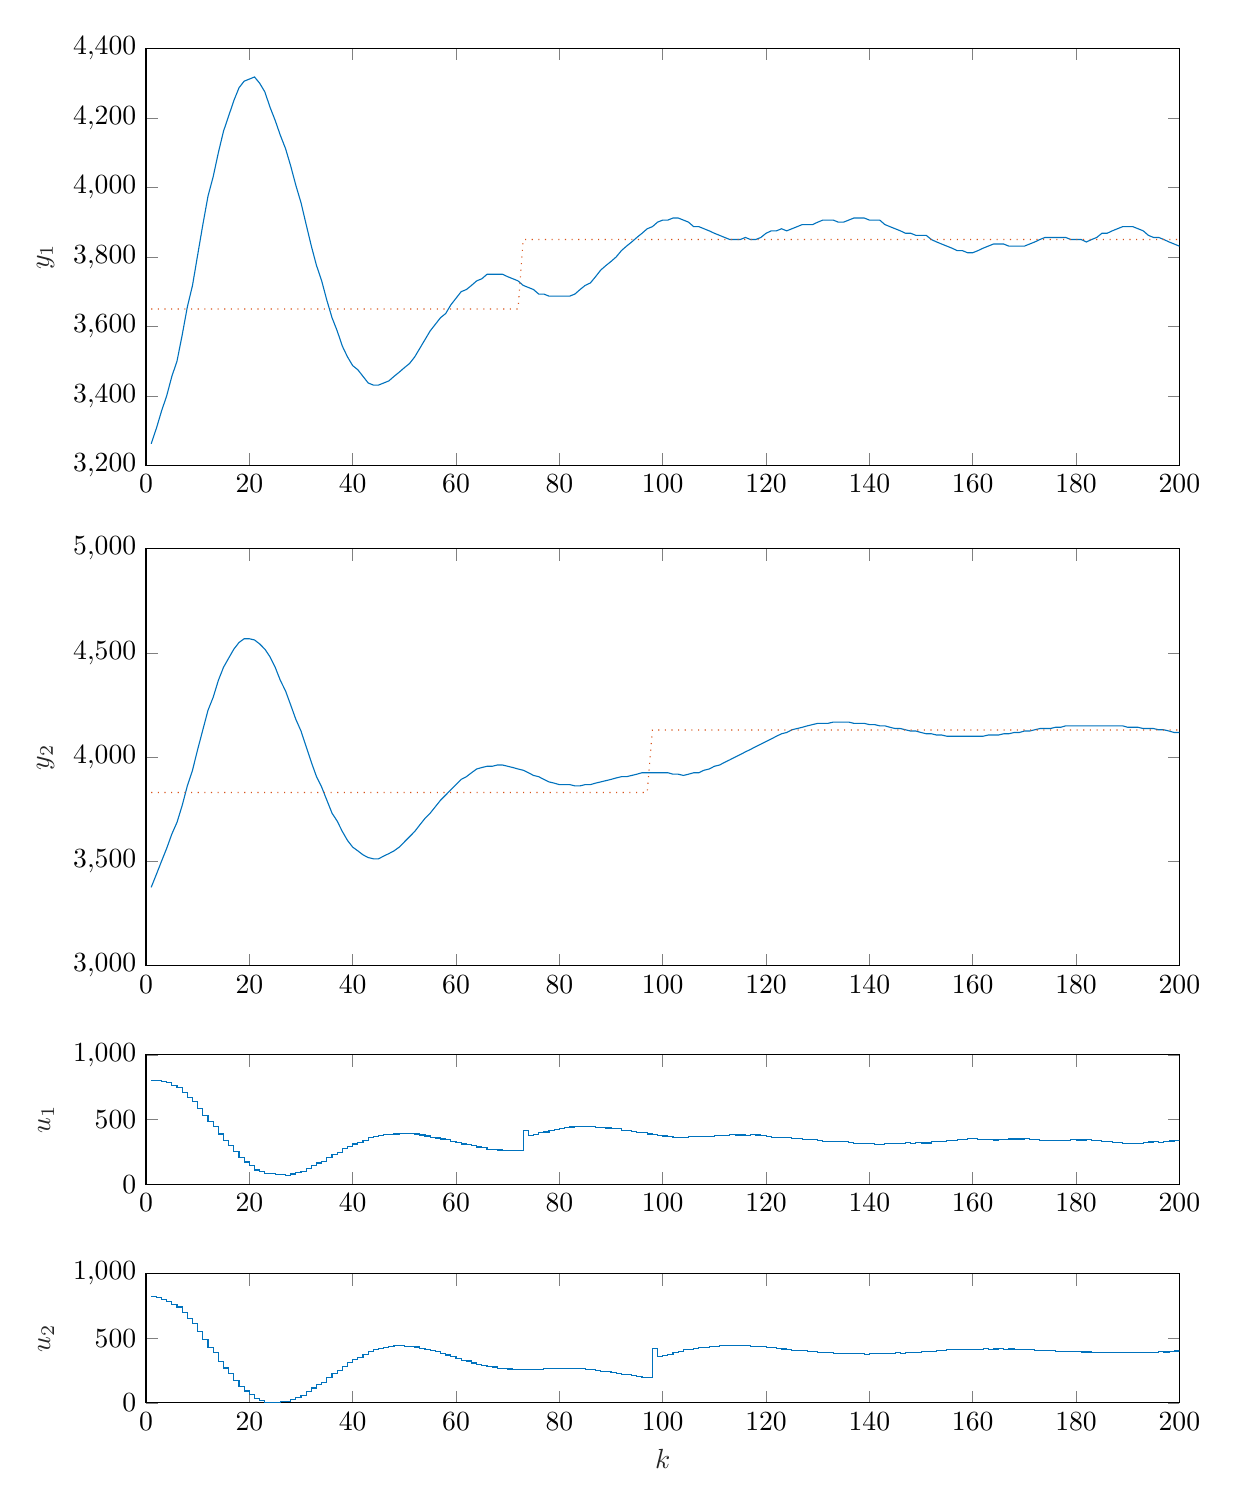
\begin{tikzpicture}

\begin{axis}[%
width=5.167in,
height=0.646in,
at={(0.646in,0.521in)},
scale only axis,
xmin=0,
xmax=200,
xtick={0,20,40,60,80,100,120,140,160,180,200},
xlabel style={font=\color{white!15!black}},
xlabel={$k$},
ymin=0,
ymax=1000,
ytick={0,500,1000},
ylabel style={font=\color{white!15!black}},
ylabel={$u_2$},
axis background/.style={fill=white}
]
\addplot[const plot, color=mycolor1, forget plot] table[row sep=crcr] {%
1	827\\
2	818\\
3	802\\
4	785\\
5	759\\
6	742\\
7	700\\
8	650\\
9	614\\
10	551\\
11	494\\
12	432\\
13	390\\
14	322\\
15	270\\
16	225\\
17	174\\
18	130\\
19	92\\
20	63\\
21	35\\
22	16\\
23	0\\
24	0\\
25	0\\
26	9\\
27	8\\
28	27\\
29	44\\
30	55\\
31	85\\
32	115\\
33	143\\
34	161\\
35	196\\
36	230\\
37	248\\
38	283\\
39	312\\
40	336\\
41	354\\
42	376\\
43	395\\
44	410\\
45	423\\
46	427\\
47	435\\
48	441\\
49	442\\
50	439\\
51	437\\
52	433\\
53	423\\
54	414\\
55	408\\
56	395\\
57	381\\
58	371\\
59	359\\
60	345\\
61	331\\
62	324\\
63	309\\
64	296\\
65	290\\
66	282\\
67	278\\
68	267\\
69	263\\
70	262\\
71	259\\
72	258\\
73	256\\
74	259\\
75	261\\
76	259\\
77	264\\
78	268\\
79	267\\
80	269\\
81	265\\
82	264\\
83	267\\
84	264\\
85	258\\
86	258\\
87	250\\
88	246\\
89	240\\
90	234\\
91	228\\
92	222\\
93	220\\
94	212\\
95	205\\
96	197\\
97	195\\
98	422\\
99	356\\
100	365\\
101	375\\
102	389\\
103	397\\
104	411\\
105	414\\
106	420\\
107	431\\
108	431\\
109	438\\
110	437\\
111	444\\
112	443\\
113	443\\
114	443\\
115	443\\
116	441\\
117	439\\
118	437\\
119	434\\
120	430\\
121	426\\
122	421\\
123	417\\
124	416\\
125	408\\
126	406\\
127	403\\
128	398\\
129	395\\
130	390\\
131	390\\
132	389\\
133	383\\
134	383\\
135	381\\
136	379\\
137	382\\
138	379\\
139	378\\
140	381\\
141	379\\
142	382\\
143	380\\
144	384\\
145	387\\
146	385\\
147	389\\
148	392\\
149	391\\
150	396\\
151	400\\
152	399\\
153	405\\
154	404\\
155	410\\
156	410\\
157	411\\
158	412\\
159	414\\
160	415\\
161	416\\
162	418\\
163	414\\
164	417\\
165	418\\
166	414\\
167	417\\
168	413\\
169	415\\
170	410\\
171	412\\
172	408\\
173	404\\
174	406\\
175	405\\
176	400\\
177	401\\
178	395\\
179	396\\
180	395\\
181	394\\
182	394\\
183	393\\
184	392\\
185	391\\
186	390\\
187	389\\
188	388\\
189	387\\
190	392\\
191	390\\
192	389\\
193	393\\
194	391\\
195	391\\
196	395\\
197	394\\
198	398\\
199	402\\
200	401\\
};
\end{axis}

\begin{axis}[%
width=5.167in,
height=0.646in,
at={(0.646in,1.615in)},
scale only axis,
xmin=0,
xmax=200,
xtick={0,20,40,60,80,100,120,140,160,180,200},
ymin=0,
ymax=1000,
ytick={0,500,1000},
ylabel style={font=\color{white!15!black}},
ylabel={$u_1$},
axis background/.style={fill=white}
]
\addplot[const plot, color=mycolor1, forget plot] table[row sep=crcr] {%
1	805\\
2	803\\
3	791\\
4	783\\
5	762\\
6	750\\
7	710\\
8	670\\
9	642\\
10	586\\
11	534\\
12	482\\
13	444\\
14	388\\
15	338\\
16	296\\
17	249\\
18	204\\
19	171\\
20	142\\
21	109\\
22	95\\
23	81\\
24	81\\
25	73\\
26	73\\
27	69\\
28	78\\
29	90\\
30	99\\
31	122\\
32	143\\
33	163\\
34	177\\
35	206\\
36	229\\
37	247\\
38	274\\
39	292\\
40	310\\
41	320\\
42	339\\
43	358\\
44	367\\
45	376\\
46	381\\
47	387\\
48	388\\
49	390\\
50	391\\
51	393\\
52	388\\
53	380\\
54	372\\
55	363\\
56	357\\
57	349\\
58	346\\
59	330\\
60	321\\
61	310\\
62	307\\
63	297\\
64	287\\
65	282\\
66	270\\
67	269\\
68	264\\
69	260\\
70	261\\
71	259\\
72	259\\
73	418\\
74	375\\
75	385\\
76	400\\
77	403\\
78	415\\
79	421\\
80	428\\
81	435\\
82	442\\
83	445\\
84	443\\
85	444\\
86	447\\
87	441\\
88	435\\
89	434\\
90	431\\
91	427\\
92	418\\
93	414\\
94	409\\
95	402\\
96	396\\
97	388\\
98	386\\
99	375\\
100	372\\
101	371\\
102	364\\
103	362\\
104	364\\
105	365\\
106	371\\
107	366\\
108	369\\
109	371\\
110	374\\
111	376\\
112	379\\
113	381\\
114	380\\
115	380\\
116	375\\
117	381\\
118	380\\
119	375\\
120	367\\
121	364\\
122	364\\
123	359\\
124	363\\
125	356\\
126	352\\
127	347\\
128	347\\
129	345\\
130	337\\
131	332\\
132	331\\
133	329\\
134	331\\
135	327\\
136	320\\
137	315\\
138	313\\
139	311\\
140	313\\
141	309\\
142	306\\
143	314\\
144	313\\
145	315\\
146	316\\
147	319\\
148	317\\
149	320\\
150	318\\
151	318\\
152	327\\
153	329\\
154	332\\
155	336\\
156	340\\
157	345\\
158	345\\
159	351\\
160	351\\
161	348\\
162	345\\
163	344\\
164	341\\
165	343\\
166	344\\
167	349\\
168	349\\
169	349\\
170	350\\
171	346\\
172	344\\
173	340\\
174	337\\
175	339\\
176	338\\
177	338\\
178	338\\
179	342\\
180	341\\
181	341\\
182	346\\
183	339\\
184	336\\
185	328\\
186	331\\
187	324\\
188	320\\
189	316\\
190	316\\
191	314\\
192	317\\
193	319\\
194	326\\
195	327\\
196	325\\
197	330\\
198	334\\
199	337\\
200	340\\
};
\end{axis}

\begin{axis}[%
width=5.167in,
height=2.084in,
at={(0.646in,2.708in)},
scale only axis,
xmin=0,
xmax=200,
xtick={0,20,40,60,80,100,120,140,160,180,200},
ymin=3000,
ymax=5000,
ytick={3000,3500,4000,4500,5000},
ylabel style={font=\color{white!15!black}},
ylabel={$y_2$},
axis background/.style={fill=white}
]
\addplot [color=mycolor1, forget plot]
  table[row sep=crcr]{%
1	3375\\
2	3437\\
3	3500\\
4	3562\\
5	3631\\
6	3687\\
7	3768\\
8	3862\\
9	3937\\
10	4037\\
11	4131\\
12	4225\\
13	4287\\
14	4368\\
15	4431\\
16	4475\\
17	4518\\
18	4550\\
19	4568\\
20	4568\\
21	4562\\
22	4543\\
23	4518\\
24	4481\\
25	4431\\
26	4368\\
27	4318\\
28	4250\\
29	4181\\
30	4125\\
31	4050\\
32	3975\\
33	3906\\
34	3856\\
35	3793\\
36	3731\\
37	3693\\
38	3643\\
39	3600\\
40	3568\\
41	3550\\
42	3531\\
43	3518\\
44	3512\\
45	3512\\
46	3525\\
47	3537\\
48	3550\\
49	3568\\
50	3593\\
51	3618\\
52	3643\\
53	3675\\
54	3706\\
55	3731\\
56	3762\\
57	3793\\
58	3818\\
59	3843\\
60	3868\\
61	3893\\
62	3906\\
63	3925\\
64	3943\\
65	3950\\
66	3956\\
67	3956\\
68	3962\\
69	3962\\
70	3956\\
71	3950\\
72	3943\\
73	3937\\
74	3925\\
75	3912\\
76	3906\\
77	3893\\
78	3881\\
79	3875\\
80	3868\\
81	3868\\
82	3868\\
83	3862\\
84	3862\\
85	3868\\
86	3868\\
87	3875\\
88	3881\\
89	3887\\
90	3893\\
91	3900\\
92	3906\\
93	3906\\
94	3912\\
95	3918\\
96	3925\\
97	3925\\
98	3925\\
99	3925\\
100	3925\\
101	3925\\
102	3918\\
103	3918\\
104	3912\\
105	3918\\
106	3925\\
107	3925\\
108	3937\\
109	3943\\
110	3956\\
111	3962\\
112	3975\\
113	3987\\
114	4000\\
115	4012\\
116	4025\\
117	4037\\
118	4050\\
119	4062\\
120	4075\\
121	4087\\
122	4100\\
123	4112\\
124	4118\\
125	4131\\
126	4137\\
127	4143\\
128	4150\\
129	4156\\
130	4162\\
131	4162\\
132	4162\\
133	4168\\
134	4168\\
135	4168\\
136	4168\\
137	4162\\
138	4162\\
139	4162\\
140	4156\\
141	4156\\
142	4150\\
143	4150\\
144	4143\\
145	4137\\
146	4137\\
147	4131\\
148	4125\\
149	4125\\
150	4118\\
151	4112\\
152	4112\\
153	4106\\
154	4106\\
155	4100\\
156	4100\\
157	4100\\
158	4100\\
159	4100\\
160	4100\\
161	4100\\
162	4100\\
163	4106\\
164	4106\\
165	4106\\
166	4112\\
167	4112\\
168	4118\\
169	4118\\
170	4125\\
171	4125\\
172	4131\\
173	4137\\
174	4137\\
175	4137\\
176	4143\\
177	4143\\
178	4150\\
179	4150\\
180	4150\\
181	4150\\
182	4150\\
183	4150\\
184	4150\\
185	4150\\
186	4150\\
187	4150\\
188	4150\\
189	4150\\
190	4143\\
191	4143\\
192	4143\\
193	4137\\
194	4137\\
195	4137\\
196	4131\\
197	4131\\
198	4125\\
199	4118\\
200	4118\\
};
\addplot [color=mycolor2, dotted, forget plot]
  table[row sep=crcr]{%
1	3830\\
2	3830\\
3	3830\\
4	3830\\
5	3830\\
6	3830\\
7	3830\\
8	3830\\
9	3830\\
10	3830\\
11	3830\\
12	3830\\
13	3830\\
14	3830\\
15	3830\\
16	3830\\
17	3830\\
18	3830\\
19	3830\\
20	3830\\
21	3830\\
22	3830\\
23	3830\\
24	3830\\
25	3830\\
26	3830\\
27	3830\\
28	3830\\
29	3830\\
30	3830\\
31	3830\\
32	3830\\
33	3830\\
34	3830\\
35	3830\\
36	3830\\
37	3830\\
38	3830\\
39	3830\\
40	3830\\
41	3830\\
42	3830\\
43	3830\\
44	3830\\
45	3830\\
46	3830\\
47	3830\\
48	3830\\
49	3830\\
50	3830\\
51	3830\\
52	3830\\
53	3830\\
54	3830\\
55	3830\\
56	3830\\
57	3830\\
58	3830\\
59	3830\\
60	3830\\
61	3830\\
62	3830\\
63	3830\\
64	3830\\
65	3830\\
66	3830\\
67	3830\\
68	3830\\
69	3830\\
70	3830\\
71	3830\\
72	3830\\
73	3830\\
74	3830\\
75	3830\\
76	3830\\
77	3830\\
78	3830\\
79	3830\\
80	3830\\
81	3830\\
82	3830\\
83	3830\\
84	3830\\
85	3830\\
86	3830\\
87	3830\\
88	3830\\
89	3830\\
90	3830\\
91	3830\\
92	3830\\
93	3830\\
94	3830\\
95	3830\\
96	3830\\
97	3830\\
98	4130\\
99	4130\\
100	4130\\
101	4130\\
102	4130\\
103	4130\\
104	4130\\
105	4130\\
106	4130\\
107	4130\\
108	4130\\
109	4130\\
110	4130\\
111	4130\\
112	4130\\
113	4130\\
114	4130\\
115	4130\\
116	4130\\
117	4130\\
118	4130\\
119	4130\\
120	4130\\
121	4130\\
122	4130\\
123	4130\\
124	4130\\
125	4130\\
126	4130\\
127	4130\\
128	4130\\
129	4130\\
130	4130\\
131	4130\\
132	4130\\
133	4130\\
134	4130\\
135	4130\\
136	4130\\
137	4130\\
138	4130\\
139	4130\\
140	4130\\
141	4130\\
142	4130\\
143	4130\\
144	4130\\
145	4130\\
146	4130\\
147	4130\\
148	4130\\
149	4130\\
150	4130\\
151	4130\\
152	4130\\
153	4130\\
154	4130\\
155	4130\\
156	4130\\
157	4130\\
158	4130\\
159	4130\\
160	4130\\
161	4130\\
162	4130\\
163	4130\\
164	4130\\
165	4130\\
166	4130\\
167	4130\\
168	4130\\
169	4130\\
170	4130\\
171	4130\\
172	4130\\
173	4130\\
174	4130\\
175	4130\\
176	4130\\
177	4130\\
178	4130\\
179	4130\\
180	4130\\
181	4130\\
182	4130\\
183	4130\\
184	4130\\
185	4130\\
186	4130\\
187	4130\\
188	4130\\
189	4130\\
190	4130\\
191	4130\\
192	4130\\
193	4130\\
194	4130\\
195	4130\\
196	4130\\
197	4130\\
198	4130\\
199	4130\\
200	4130\\
};
\end{axis}

\begin{axis}[%
width=5.167in,
height=2.084in,
at={(0.646in,5.209in)},
scale only axis,
xmin=0,
xmax=200,
xtick={0,20,40,60,80,100,120,140,160,180,200},
ymin=3200,
ymax=4400,
ytick={3200,3400,3600,3800,4000,4200,4400},
ylabel style={font=\color{white!15!black}},
ylabel={$y_1$},
axis background/.style={fill=white}
]
\addplot [color=mycolor1, forget plot]
  table[row sep=crcr]{%
1	3262\\
2	3306\\
3	3356\\
4	3400\\
5	3456\\
6	3500\\
7	3575\\
8	3656\\
9	3718\\
10	3806\\
11	3893\\
12	3975\\
13	4031\\
14	4100\\
15	4162\\
16	4206\\
17	4250\\
18	4287\\
19	4306\\
20	4312\\
21	4318\\
22	4300\\
23	4275\\
24	4231\\
25	4193\\
26	4150\\
27	4112\\
28	4062\\
29	4006\\
30	3956\\
31	3893\\
32	3831\\
33	3775\\
34	3731\\
35	3675\\
36	3625\\
37	3587\\
38	3543\\
39	3512\\
40	3487\\
41	3475\\
42	3456\\
43	3437\\
44	3431\\
45	3431\\
46	3437\\
47	3443\\
48	3456\\
49	3468\\
50	3481\\
51	3493\\
52	3512\\
53	3537\\
54	3562\\
55	3587\\
56	3606\\
57	3625\\
58	3637\\
59	3662\\
60	3681\\
61	3700\\
62	3706\\
63	3718\\
64	3731\\
65	3737\\
66	3750\\
67	3750\\
68	3750\\
69	3750\\
70	3743\\
71	3737\\
72	3731\\
73	3718\\
74	3712\\
75	3706\\
76	3693\\
77	3693\\
78	3687\\
79	3687\\
80	3687\\
81	3687\\
82	3687\\
83	3693\\
84	3706\\
85	3718\\
86	3725\\
87	3743\\
88	3762\\
89	3775\\
90	3787\\
91	3800\\
92	3818\\
93	3831\\
94	3843\\
95	3856\\
96	3868\\
97	3881\\
98	3887\\
99	3900\\
100	3906\\
101	3906\\
102	3912\\
103	3912\\
104	3906\\
105	3900\\
106	3887\\
107	3887\\
108	3881\\
109	3875\\
110	3868\\
111	3862\\
112	3856\\
113	3850\\
114	3850\\
115	3850\\
116	3856\\
117	3850\\
118	3850\\
119	3856\\
120	3868\\
121	3875\\
122	3875\\
123	3881\\
124	3875\\
125	3881\\
126	3887\\
127	3893\\
128	3893\\
129	3893\\
130	3900\\
131	3906\\
132	3906\\
133	3906\\
134	3900\\
135	3900\\
136	3906\\
137	3912\\
138	3912\\
139	3912\\
140	3906\\
141	3906\\
142	3906\\
143	3893\\
144	3887\\
145	3881\\
146	3875\\
147	3868\\
148	3868\\
149	3862\\
150	3862\\
151	3862\\
152	3850\\
153	3843\\
154	3837\\
155	3831\\
156	3825\\
157	3818\\
158	3818\\
159	3812\\
160	3812\\
161	3818\\
162	3825\\
163	3831\\
164	3837\\
165	3837\\
166	3837\\
167	3831\\
168	3831\\
169	3831\\
170	3831\\
171	3837\\
172	3843\\
173	3850\\
174	3856\\
175	3856\\
176	3856\\
177	3856\\
178	3856\\
179	3850\\
180	3850\\
181	3850\\
182	3843\\
183	3850\\
184	3856\\
185	3868\\
186	3868\\
187	3875\\
188	3881\\
189	3887\\
190	3887\\
191	3887\\
192	3881\\
193	3875\\
194	3862\\
195	3856\\
196	3856\\
197	3850\\
198	3843\\
199	3837\\
200	3831\\
};
\addplot [color=mycolor2, dotted, forget plot]
  table[row sep=crcr]{%
1	3650\\
2	3650\\
3	3650\\
4	3650\\
5	3650\\
6	3650\\
7	3650\\
8	3650\\
9	3650\\
10	3650\\
11	3650\\
12	3650\\
13	3650\\
14	3650\\
15	3650\\
16	3650\\
17	3650\\
18	3650\\
19	3650\\
20	3650\\
21	3650\\
22	3650\\
23	3650\\
24	3650\\
25	3650\\
26	3650\\
27	3650\\
28	3650\\
29	3650\\
30	3650\\
31	3650\\
32	3650\\
33	3650\\
34	3650\\
35	3650\\
36	3650\\
37	3650\\
38	3650\\
39	3650\\
40	3650\\
41	3650\\
42	3650\\
43	3650\\
44	3650\\
45	3650\\
46	3650\\
47	3650\\
48	3650\\
49	3650\\
50	3650\\
51	3650\\
52	3650\\
53	3650\\
54	3650\\
55	3650\\
56	3650\\
57	3650\\
58	3650\\
59	3650\\
60	3650\\
61	3650\\
62	3650\\
63	3650\\
64	3650\\
65	3650\\
66	3650\\
67	3650\\
68	3650\\
69	3650\\
70	3650\\
71	3650\\
72	3650\\
73	3850\\
74	3850\\
75	3850\\
76	3850\\
77	3850\\
78	3850\\
79	3850\\
80	3850\\
81	3850\\
82	3850\\
83	3850\\
84	3850\\
85	3850\\
86	3850\\
87	3850\\
88	3850\\
89	3850\\
90	3850\\
91	3850\\
92	3850\\
93	3850\\
94	3850\\
95	3850\\
96	3850\\
97	3850\\
98	3850\\
99	3850\\
100	3850\\
101	3850\\
102	3850\\
103	3850\\
104	3850\\
105	3850\\
106	3850\\
107	3850\\
108	3850\\
109	3850\\
110	3850\\
111	3850\\
112	3850\\
113	3850\\
114	3850\\
115	3850\\
116	3850\\
117	3850\\
118	3850\\
119	3850\\
120	3850\\
121	3850\\
122	3850\\
123	3850\\
124	3850\\
125	3850\\
126	3850\\
127	3850\\
128	3850\\
129	3850\\
130	3850\\
131	3850\\
132	3850\\
133	3850\\
134	3850\\
135	3850\\
136	3850\\
137	3850\\
138	3850\\
139	3850\\
140	3850\\
141	3850\\
142	3850\\
143	3850\\
144	3850\\
145	3850\\
146	3850\\
147	3850\\
148	3850\\
149	3850\\
150	3850\\
151	3850\\
152	3850\\
153	3850\\
154	3850\\
155	3850\\
156	3850\\
157	3850\\
158	3850\\
159	3850\\
160	3850\\
161	3850\\
162	3850\\
163	3850\\
164	3850\\
165	3850\\
166	3850\\
167	3850\\
168	3850\\
169	3850\\
170	3850\\
171	3850\\
172	3850\\
173	3850\\
174	3850\\
175	3850\\
176	3850\\
177	3850\\
178	3850\\
179	3850\\
180	3850\\
181	3850\\
182	3850\\
183	3850\\
184	3850\\
185	3850\\
186	3850\\
187	3850\\
188	3850\\
189	3850\\
190	3850\\
191	3850\\
192	3850\\
193	3850\\
194	3850\\
195	3850\\
196	3850\\
197	3850\\
198	3850\\
199	3850\\
200	3850\\
};
\end{axis}
\end{tikzpicture}%
\caption{Regulator PID dla $K=\num{0.5}$ $T_{\mathrm{i}}=\num{45}$ $T_{\mathrm{d}}=\num{2}$.}
\label{Z3PID}
\end{figure}


\chapter{Podpunkt 4}
Odpowiedzi skokowe procesu zbadane zostały dla skoku sygnału sterującego G1 o 20 z początkowej wartości 30 z pomiarem na T1 i T3. Na rys.~\ref{Z4step} zamieszczono wyznaczone odpowiedzi dla wszystkich torów.

\begin{figure}[ht]
\centering
% This file was created by matlab2tikz.
%
%The latest updates can be retrieved from
%  http://www.mathworks.com/matlabcentral/fileexchange/22022-matlab2tikz-matlab2tikz
%where you can also make suggestions and rate matlab2tikz.
%
\definecolor{mycolor1}{rgb}{0.00000,0.44700,0.74100}%
\definecolor{mycolor2}{rgb}{0.85000,0.32500,0.09800}%
%
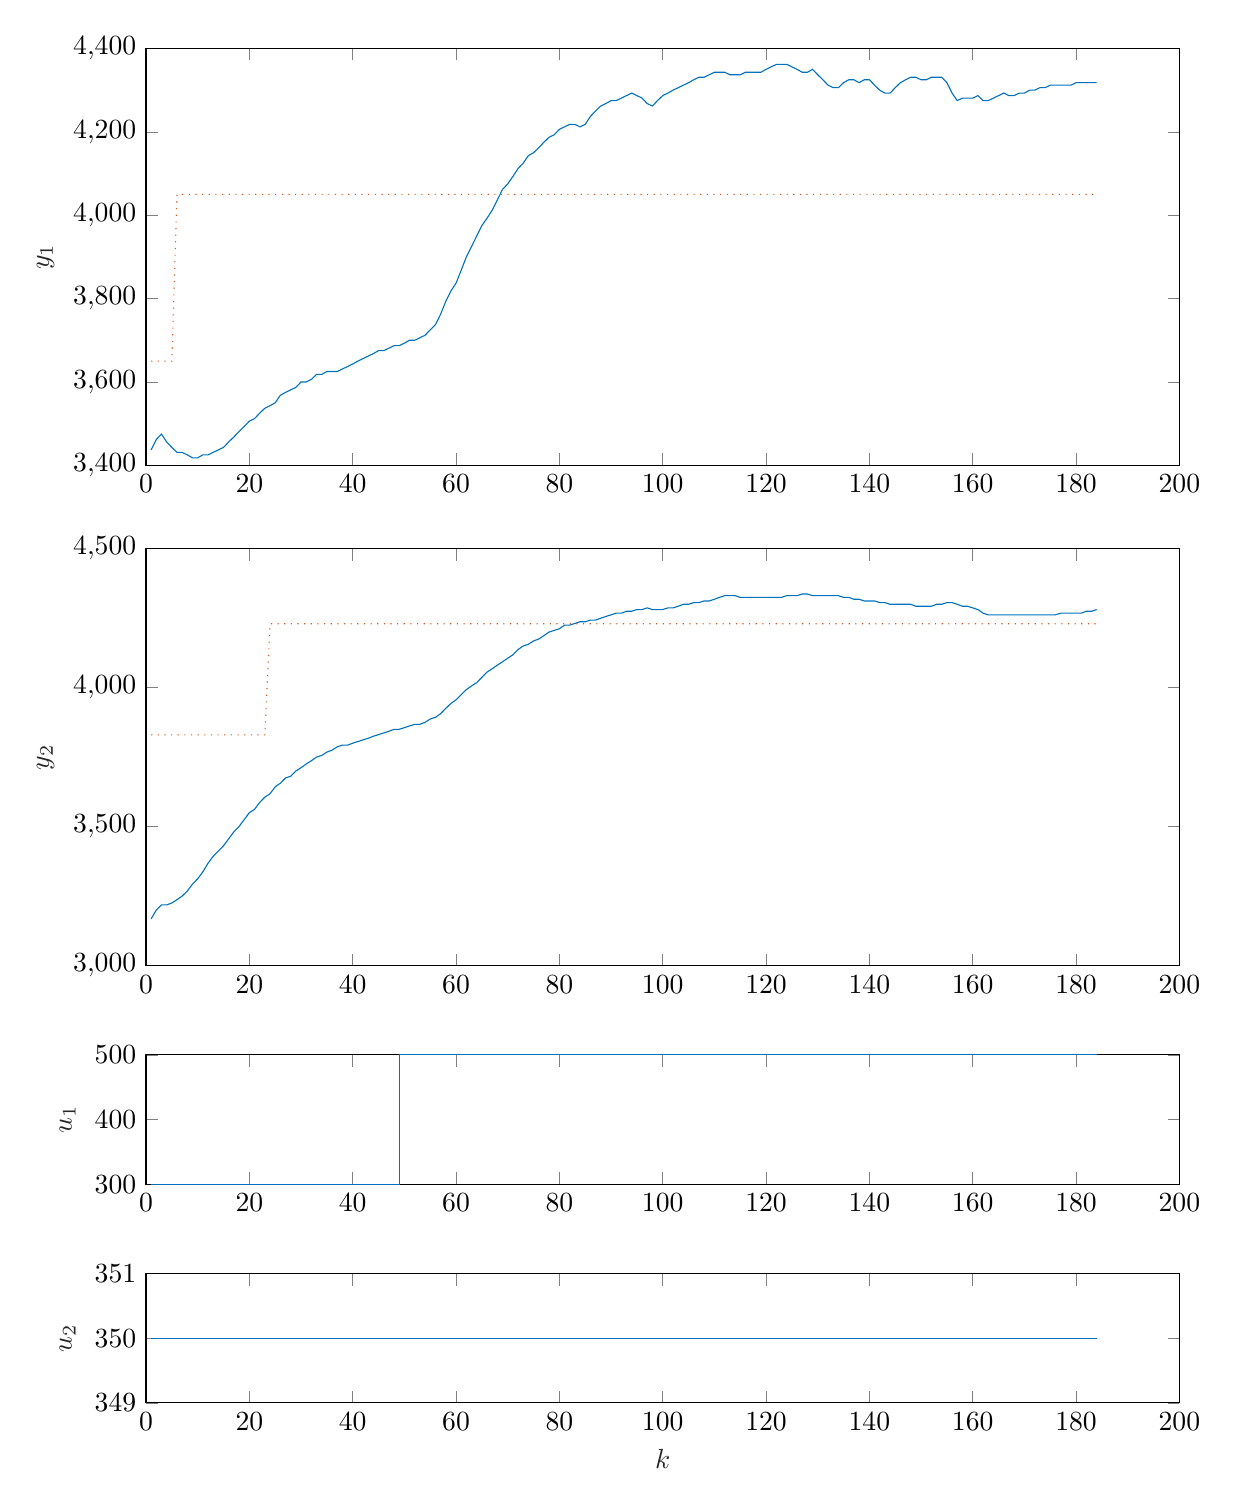
\begin{tikzpicture}

\begin{axis}[%
width=5.167in,
height=0.646in,
at={(0.646in,0.521in)},
scale only axis,
xmin=0,
xmax=200,
xtick={0,20,40,60,80,100,120,140,160,180,200},
xlabel style={font=\color{white!15!black}},
xlabel={$k$},
ymin=349,
ymax=351,
ytick={349,350,351},
ylabel style={font=\color{white!15!black}},
ylabel={$u_2$},
axis background/.style={fill=white}
]
\addplot[const plot, color=mycolor1, forget plot] table[row sep=crcr] {%
1	350\\
2	350\\
3	350\\
4	350\\
5	350\\
6	350\\
7	350\\
8	350\\
9	350\\
10	350\\
11	350\\
12	350\\
13	350\\
14	350\\
15	350\\
16	350\\
17	350\\
18	350\\
19	350\\
20	350\\
21	350\\
22	350\\
23	350\\
24	350\\
25	350\\
26	350\\
27	350\\
28	350\\
29	350\\
30	350\\
31	350\\
32	350\\
33	350\\
34	350\\
35	350\\
36	350\\
37	350\\
38	350\\
39	350\\
40	350\\
41	350\\
42	350\\
43	350\\
44	350\\
45	350\\
46	350\\
47	350\\
48	350\\
49	350\\
50	350\\
51	350\\
52	350\\
53	350\\
54	350\\
55	350\\
56	350\\
57	350\\
58	350\\
59	350\\
60	350\\
61	350\\
62	350\\
63	350\\
64	350\\
65	350\\
66	350\\
67	350\\
68	350\\
69	350\\
70	350\\
71	350\\
72	350\\
73	350\\
74	350\\
75	350\\
76	350\\
77	350\\
78	350\\
79	350\\
80	350\\
81	350\\
82	350\\
83	350\\
84	350\\
85	350\\
86	350\\
87	350\\
88	350\\
89	350\\
90	350\\
91	350\\
92	350\\
93	350\\
94	350\\
95	350\\
96	350\\
97	350\\
98	350\\
99	350\\
100	350\\
101	350\\
102	350\\
103	350\\
104	350\\
105	350\\
106	350\\
107	350\\
108	350\\
109	350\\
110	350\\
111	350\\
112	350\\
113	350\\
114	350\\
115	350\\
116	350\\
117	350\\
118	350\\
119	350\\
120	350\\
121	350\\
122	350\\
123	350\\
124	350\\
125	350\\
126	350\\
127	350\\
128	350\\
129	350\\
130	350\\
131	350\\
132	350\\
133	350\\
134	350\\
135	350\\
136	350\\
137	350\\
138	350\\
139	350\\
140	350\\
141	350\\
142	350\\
143	350\\
144	350\\
145	350\\
146	350\\
147	350\\
148	350\\
149	350\\
150	350\\
151	350\\
152	350\\
153	350\\
154	350\\
155	350\\
156	350\\
157	350\\
158	350\\
159	350\\
160	350\\
161	350\\
162	350\\
163	350\\
164	350\\
165	350\\
166	350\\
167	350\\
168	350\\
169	350\\
170	350\\
171	350\\
172	350\\
173	350\\
174	350\\
175	350\\
176	350\\
177	350\\
178	350\\
179	350\\
180	350\\
181	350\\
182	350\\
183	350\\
184	350\\
};
\end{axis}

\begin{axis}[%
width=5.167in,
height=0.646in,
at={(0.646in,1.615in)},
scale only axis,
xmin=0,
xmax=200,
xtick={0,20,40,60,80,100,120,140,160,180,200},
ymin=300,
ymax=500,
ytick={300,400,500},
ylabel style={font=\color{white!15!black}},
ylabel={$u_1$},
axis background/.style={fill=white}
]
\addplot[const plot, color=mycolor1, forget plot] table[row sep=crcr] {%
1	300\\
2	300\\
3	300\\
4	300\\
5	300\\
6	300\\
7	300\\
8	300\\
9	300\\
10	300\\
11	300\\
12	300\\
13	300\\
14	300\\
15	300\\
16	300\\
17	300\\
18	300\\
19	300\\
20	300\\
21	300\\
22	300\\
23	300\\
24	300\\
25	300\\
26	300\\
27	300\\
28	300\\
29	300\\
30	300\\
31	300\\
32	300\\
33	300\\
34	300\\
35	300\\
36	300\\
37	300\\
38	300\\
39	300\\
40	300\\
41	300\\
42	300\\
43	300\\
44	300\\
45	300\\
46	300\\
47	300\\
48	300\\
49	500\\
50	500\\
51	500\\
52	500\\
53	500\\
54	500\\
55	500\\
56	500\\
57	500\\
58	500\\
59	500\\
60	500\\
61	500\\
62	500\\
63	500\\
64	500\\
65	500\\
66	500\\
67	500\\
68	500\\
69	500\\
70	500\\
71	500\\
72	500\\
73	500\\
74	500\\
75	500\\
76	500\\
77	500\\
78	500\\
79	500\\
80	500\\
81	500\\
82	500\\
83	500\\
84	500\\
85	500\\
86	500\\
87	500\\
88	500\\
89	500\\
90	500\\
91	500\\
92	500\\
93	500\\
94	500\\
95	500\\
96	500\\
97	500\\
98	500\\
99	500\\
100	500\\
101	500\\
102	500\\
103	500\\
104	500\\
105	500\\
106	500\\
107	500\\
108	500\\
109	500\\
110	500\\
111	500\\
112	500\\
113	500\\
114	500\\
115	500\\
116	500\\
117	500\\
118	500\\
119	500\\
120	500\\
121	500\\
122	500\\
123	500\\
124	500\\
125	500\\
126	500\\
127	500\\
128	500\\
129	500\\
130	500\\
131	500\\
132	500\\
133	500\\
134	500\\
135	500\\
136	500\\
137	500\\
138	500\\
139	500\\
140	500\\
141	500\\
142	500\\
143	500\\
144	500\\
145	500\\
146	500\\
147	500\\
148	500\\
149	500\\
150	500\\
151	500\\
152	500\\
153	500\\
154	500\\
155	500\\
156	500\\
157	500\\
158	500\\
159	500\\
160	500\\
161	500\\
162	500\\
163	500\\
164	500\\
165	500\\
166	500\\
167	500\\
168	500\\
169	500\\
170	500\\
171	500\\
172	500\\
173	500\\
174	500\\
175	500\\
176	500\\
177	500\\
178	500\\
179	500\\
180	500\\
181	500\\
182	500\\
183	500\\
184	500\\
};
\end{axis}

\begin{axis}[%
width=5.167in,
height=2.084in,
at={(0.646in,2.708in)},
scale only axis,
xmin=0,
xmax=200,
xtick={0,20,40,60,80,100,120,140,160,180,200},
ymin=3000,
ymax=4500,
ytick={3000,3500,4000,4500},
ylabel style={font=\color{white!15!black}},
ylabel={$y_2$},
axis background/.style={fill=white}
]
\addplot [color=mycolor1, forget plot]
  table[row sep=crcr]{%
1	3168\\
2	3200\\
3	3218\\
4	3218\\
5	3225\\
6	3237\\
7	3250\\
8	3268\\
9	3293\\
10	3312\\
11	3337\\
12	3368\\
13	3393\\
14	3412\\
15	3431\\
16	3456\\
17	3481\\
18	3500\\
19	3525\\
20	3550\\
21	3562\\
22	3587\\
23	3606\\
24	3618\\
25	3643\\
26	3656\\
27	3675\\
28	3681\\
29	3700\\
30	3712\\
31	3725\\
32	3737\\
33	3750\\
34	3756\\
35	3768\\
36	3775\\
37	3787\\
38	3793\\
39	3793\\
40	3800\\
41	3806\\
42	3812\\
43	3818\\
44	3825\\
45	3831\\
46	3837\\
47	3843\\
48	3850\\
49	3850\\
50	3856\\
51	3862\\
52	3868\\
53	3868\\
54	3875\\
55	3887\\
56	3893\\
57	3906\\
58	3925\\
59	3943\\
60	3956\\
61	3975\\
62	3993\\
63	4006\\
64	4018\\
65	4037\\
66	4056\\
67	4068\\
68	4081\\
69	4093\\
70	4106\\
71	4118\\
72	4137\\
73	4150\\
74	4156\\
75	4168\\
76	4175\\
77	4187\\
78	4200\\
79	4206\\
80	4212\\
81	4225\\
82	4225\\
83	4231\\
84	4237\\
85	4237\\
86	4243\\
87	4243\\
88	4250\\
89	4256\\
90	4262\\
91	4268\\
92	4268\\
93	4275\\
94	4275\\
95	4281\\
96	4281\\
97	4287\\
98	4281\\
99	4281\\
100	4281\\
101	4287\\
102	4287\\
103	4293\\
104	4300\\
105	4300\\
106	4306\\
107	4306\\
108	4312\\
109	4312\\
110	4318\\
111	4325\\
112	4331\\
113	4331\\
114	4331\\
115	4325\\
116	4325\\
117	4325\\
118	4325\\
119	4325\\
120	4325\\
121	4325\\
122	4325\\
123	4325\\
124	4331\\
125	4331\\
126	4331\\
127	4337\\
128	4337\\
129	4331\\
130	4331\\
131	4331\\
132	4331\\
133	4331\\
134	4331\\
135	4325\\
136	4325\\
137	4318\\
138	4318\\
139	4312\\
140	4312\\
141	4312\\
142	4306\\
143	4306\\
144	4300\\
145	4300\\
146	4300\\
147	4300\\
148	4300\\
149	4293\\
150	4293\\
151	4293\\
152	4293\\
153	4300\\
154	4300\\
155	4306\\
156	4306\\
157	4300\\
158	4293\\
159	4293\\
160	4287\\
161	4281\\
162	4268\\
163	4262\\
164	4262\\
165	4262\\
166	4262\\
167	4262\\
168	4262\\
169	4262\\
170	4262\\
171	4262\\
172	4262\\
173	4262\\
174	4262\\
175	4262\\
176	4262\\
177	4268\\
178	4268\\
179	4268\\
180	4268\\
181	4268\\
182	4275\\
183	4275\\
184	4281\\
};
\addplot [color=mycolor2, dotted, forget plot]
  table[row sep=crcr]{%
1	3830\\
2	3830\\
3	3830\\
4	3830\\
5	3830\\
6	3830\\
7	3830\\
8	3830\\
9	3830\\
10	3830\\
11	3830\\
12	3830\\
13	3830\\
14	3830\\
15	3830\\
16	3830\\
17	3830\\
18	3830\\
19	3830\\
20	3830\\
21	3830\\
22	3830\\
23	3830\\
24	4230\\
25	4230\\
26	4230\\
27	4230\\
28	4230\\
29	4230\\
30	4230\\
31	4230\\
32	4230\\
33	4230\\
34	4230\\
35	4230\\
36	4230\\
37	4230\\
38	4230\\
39	4230\\
40	4230\\
41	4230\\
42	4230\\
43	4230\\
44	4230\\
45	4230\\
46	4230\\
47	4230\\
48	4230\\
49	4230\\
50	4230\\
51	4230\\
52	4230\\
53	4230\\
54	4230\\
55	4230\\
56	4230\\
57	4230\\
58	4230\\
59	4230\\
60	4230\\
61	4230\\
62	4230\\
63	4230\\
64	4230\\
65	4230\\
66	4230\\
67	4230\\
68	4230\\
69	4230\\
70	4230\\
71	4230\\
72	4230\\
73	4230\\
74	4230\\
75	4230\\
76	4230\\
77	4230\\
78	4230\\
79	4230\\
80	4230\\
81	4230\\
82	4230\\
83	4230\\
84	4230\\
85	4230\\
86	4230\\
87	4230\\
88	4230\\
89	4230\\
90	4230\\
91	4230\\
92	4230\\
93	4230\\
94	4230\\
95	4230\\
96	4230\\
97	4230\\
98	4230\\
99	4230\\
100	4230\\
101	4230\\
102	4230\\
103	4230\\
104	4230\\
105	4230\\
106	4230\\
107	4230\\
108	4230\\
109	4230\\
110	4230\\
111	4230\\
112	4230\\
113	4230\\
114	4230\\
115	4230\\
116	4230\\
117	4230\\
118	4230\\
119	4230\\
120	4230\\
121	4230\\
122	4230\\
123	4230\\
124	4230\\
125	4230\\
126	4230\\
127	4230\\
128	4230\\
129	4230\\
130	4230\\
131	4230\\
132	4230\\
133	4230\\
134	4230\\
135	4230\\
136	4230\\
137	4230\\
138	4230\\
139	4230\\
140	4230\\
141	4230\\
142	4230\\
143	4230\\
144	4230\\
145	4230\\
146	4230\\
147	4230\\
148	4230\\
149	4230\\
150	4230\\
151	4230\\
152	4230\\
153	4230\\
154	4230\\
155	4230\\
156	4230\\
157	4230\\
158	4230\\
159	4230\\
160	4230\\
161	4230\\
162	4230\\
163	4230\\
164	4230\\
165	4230\\
166	4230\\
167	4230\\
168	4230\\
169	4230\\
170	4230\\
171	4230\\
172	4230\\
173	4230\\
174	4230\\
175	4230\\
176	4230\\
177	4230\\
178	4230\\
179	4230\\
180	4230\\
181	4230\\
182	4230\\
183	4230\\
184	4230\\
};
\end{axis}

\begin{axis}[%
width=5.167in,
height=2.084in,
at={(0.646in,5.209in)},
scale only axis,
xmin=0,
xmax=200,
xtick={0,20,40,60,80,100,120,140,160,180,200},
ymin=3400,
ymax=4400,
ytick={3400,3600,3800,4000,4200,4400},
ylabel style={font=\color{white!15!black}},
ylabel={$y_1$},
axis background/.style={fill=white}
]
\addplot [color=mycolor1, forget plot]
  table[row sep=crcr]{%
1	3437\\
2	3462\\
3	3475\\
4	3456\\
5	3443\\
6	3431\\
7	3431\\
8	3425\\
9	3418\\
10	3418\\
11	3425\\
12	3425\\
13	3431\\
14	3437\\
15	3443\\
16	3456\\
17	3468\\
18	3481\\
19	3493\\
20	3506\\
21	3512\\
22	3525\\
23	3537\\
24	3543\\
25	3550\\
26	3568\\
27	3575\\
28	3581\\
29	3587\\
30	3600\\
31	3600\\
32	3606\\
33	3618\\
34	3618\\
35	3625\\
36	3625\\
37	3625\\
38	3631\\
39	3637\\
40	3643\\
41	3650\\
42	3656\\
43	3662\\
44	3668\\
45	3675\\
46	3675\\
47	3681\\
48	3687\\
49	3687\\
50	3693\\
51	3700\\
52	3700\\
53	3706\\
54	3712\\
55	3725\\
56	3737\\
57	3762\\
58	3793\\
59	3818\\
60	3837\\
61	3868\\
62	3900\\
63	3925\\
64	3950\\
65	3975\\
66	3993\\
67	4012\\
68	4037\\
69	4062\\
70	4075\\
71	4093\\
72	4112\\
73	4125\\
74	4143\\
75	4150\\
76	4162\\
77	4175\\
78	4187\\
79	4193\\
80	4206\\
81	4212\\
82	4218\\
83	4218\\
84	4212\\
85	4218\\
86	4237\\
87	4250\\
88	4262\\
89	4268\\
90	4275\\
91	4275\\
92	4281\\
93	4287\\
94	4293\\
95	4287\\
96	4281\\
97	4268\\
98	4262\\
99	4275\\
100	4287\\
101	4293\\
102	4300\\
103	4306\\
104	4312\\
105	4318\\
106	4325\\
107	4331\\
108	4331\\
109	4337\\
110	4343\\
111	4343\\
112	4343\\
113	4337\\
114	4337\\
115	4337\\
116	4343\\
117	4343\\
118	4343\\
119	4343\\
120	4350\\
121	4356\\
122	4362\\
123	4362\\
124	4362\\
125	4356\\
126	4350\\
127	4343\\
128	4343\\
129	4350\\
130	4337\\
131	4325\\
132	4312\\
133	4306\\
134	4306\\
135	4318\\
136	4325\\
137	4325\\
138	4318\\
139	4325\\
140	4325\\
141	4312\\
142	4300\\
143	4293\\
144	4293\\
145	4306\\
146	4318\\
147	4325\\
148	4331\\
149	4331\\
150	4325\\
151	4325\\
152	4331\\
153	4331\\
154	4331\\
155	4318\\
156	4293\\
157	4275\\
158	4281\\
159	4281\\
160	4281\\
161	4287\\
162	4275\\
163	4275\\
164	4281\\
165	4287\\
166	4293\\
167	4287\\
168	4287\\
169	4293\\
170	4293\\
171	4300\\
172	4300\\
173	4306\\
174	4306\\
175	4312\\
176	4312\\
177	4312\\
178	4312\\
179	4312\\
180	4318\\
181	4318\\
182	4318\\
183	4318\\
184	4318\\
};
\addplot [color=mycolor2, dotted, forget plot]
  table[row sep=crcr]{%
1	3650\\
2	3650\\
3	3650\\
4	3650\\
5	3650\\
6	4050\\
7	4050\\
8	4050\\
9	4050\\
10	4050\\
11	4050\\
12	4050\\
13	4050\\
14	4050\\
15	4050\\
16	4050\\
17	4050\\
18	4050\\
19	4050\\
20	4050\\
21	4050\\
22	4050\\
23	4050\\
24	4050\\
25	4050\\
26	4050\\
27	4050\\
28	4050\\
29	4050\\
30	4050\\
31	4050\\
32	4050\\
33	4050\\
34	4050\\
35	4050\\
36	4050\\
37	4050\\
38	4050\\
39	4050\\
40	4050\\
41	4050\\
42	4050\\
43	4050\\
44	4050\\
45	4050\\
46	4050\\
47	4050\\
48	4050\\
49	4050\\
50	4050\\
51	4050\\
52	4050\\
53	4050\\
54	4050\\
55	4050\\
56	4050\\
57	4050\\
58	4050\\
59	4050\\
60	4050\\
61	4050\\
62	4050\\
63	4050\\
64	4050\\
65	4050\\
66	4050\\
67	4050\\
68	4050\\
69	4050\\
70	4050\\
71	4050\\
72	4050\\
73	4050\\
74	4050\\
75	4050\\
76	4050\\
77	4050\\
78	4050\\
79	4050\\
80	4050\\
81	4050\\
82	4050\\
83	4050\\
84	4050\\
85	4050\\
86	4050\\
87	4050\\
88	4050\\
89	4050\\
90	4050\\
91	4050\\
92	4050\\
93	4050\\
94	4050\\
95	4050\\
96	4050\\
97	4050\\
98	4050\\
99	4050\\
100	4050\\
101	4050\\
102	4050\\
103	4050\\
104	4050\\
105	4050\\
106	4050\\
107	4050\\
108	4050\\
109	4050\\
110	4050\\
111	4050\\
112	4050\\
113	4050\\
114	4050\\
115	4050\\
116	4050\\
117	4050\\
118	4050\\
119	4050\\
120	4050\\
121	4050\\
122	4050\\
123	4050\\
124	4050\\
125	4050\\
126	4050\\
127	4050\\
128	4050\\
129	4050\\
130	4050\\
131	4050\\
132	4050\\
133	4050\\
134	4050\\
135	4050\\
136	4050\\
137	4050\\
138	4050\\
139	4050\\
140	4050\\
141	4050\\
142	4050\\
143	4050\\
144	4050\\
145	4050\\
146	4050\\
147	4050\\
148	4050\\
149	4050\\
150	4050\\
151	4050\\
152	4050\\
153	4050\\
154	4050\\
155	4050\\
156	4050\\
157	4050\\
158	4050\\
159	4050\\
160	4050\\
161	4050\\
162	4050\\
163	4050\\
164	4050\\
165	4050\\
166	4050\\
167	4050\\
168	4050\\
169	4050\\
170	4050\\
171	4050\\
172	4050\\
173	4050\\
174	4050\\
175	4050\\
176	4050\\
177	4050\\
178	4050\\
179	4050\\
180	4050\\
181	4050\\
182	4050\\
183	4050\\
184	4050\\
};
\end{axis}
\end{tikzpicture}%
\caption{Odpowiedzi dla skoku sygnału sterującego G1 z punktu pracy o $\triangle U = 20$.}
\label{Z4steps}
\end{figure}

\begin{figure}[ht]
\centering
% This file was created by matlab2tikz.
%
%The latest updates can be retrieved from
%  http://www.mathworks.com/matlabcentral/fileexchange/22022-matlab2tikz-matlab2tikz
%where you can also make suggestions and rate matlab2tikz.
%
\definecolor{mycolor1}{rgb}{0.00000,0.44700,0.74100}%
%
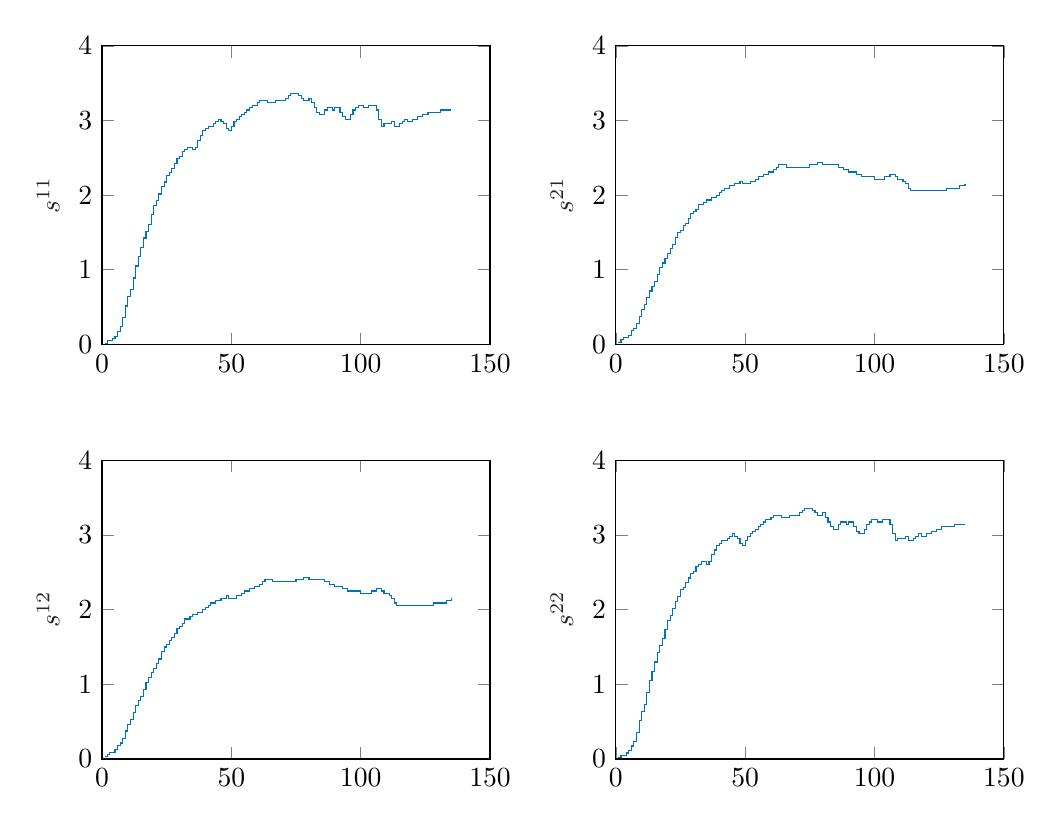
\begin{tikzpicture}

\begin{axis}[%
width=1.94in,
height=1.493in,
at={(0.758in,2.554in)},
scale only axis,
xmin=0,
xmax=150,
ymin=0,
ymax=4,
ylabel style={font=\color{white!15!black}},
ylabel={$s^{11}$},
axis background/.style={fill=white}
]
\addplot[const plot, color=mycolor1, forget plot] table[row sep=crcr] {%
1	0.015\\
2	0.05\\
3	0.05\\
4	0.08\\
5	0.11\\
6	0.175\\
7	0.235\\
8	0.36\\
9	0.515\\
10	0.64\\
11	0.735\\
12	0.89\\
13	1.05\\
14	1.175\\
15	1.3\\
16	1.425\\
17	1.515\\
18	1.61\\
19	1.735\\
20	1.86\\
21	1.925\\
22	2.015\\
23	2.11\\
24	2.175\\
25	2.265\\
26	2.3\\
27	2.36\\
28	2.425\\
29	2.485\\
30	2.515\\
31	2.58\\
32	2.61\\
33	2.64\\
34	2.64\\
35	2.61\\
36	2.64\\
37	2.735\\
38	2.8\\
39	2.86\\
40	2.89\\
41	2.925\\
42	2.925\\
43	2.955\\
44	2.985\\
45	3.015\\
46	2.985\\
47	2.955\\
48	2.89\\
49	2.86\\
50	2.925\\
51	2.985\\
52	3.015\\
53	3.05\\
54	3.08\\
55	3.11\\
56	3.14\\
57	3.175\\
58	3.205\\
59	3.205\\
60	3.235\\
61	3.265\\
62	3.265\\
63	3.265\\
64	3.235\\
65	3.235\\
66	3.235\\
67	3.265\\
68	3.265\\
69	3.265\\
70	3.265\\
71	3.3\\
72	3.33\\
73	3.36\\
74	3.36\\
75	3.36\\
76	3.33\\
77	3.3\\
78	3.265\\
79	3.265\\
80	3.3\\
81	3.235\\
82	3.175\\
83	3.11\\
84	3.08\\
85	3.08\\
86	3.14\\
87	3.175\\
88	3.175\\
89	3.14\\
90	3.175\\
91	3.175\\
92	3.11\\
93	3.05\\
94	3.015\\
95	3.015\\
96	3.08\\
97	3.14\\
98	3.175\\
99	3.205\\
100	3.205\\
101	3.175\\
102	3.175\\
103	3.205\\
104	3.205\\
105	3.205\\
106	3.14\\
107	3.015\\
108	2.925\\
109	2.955\\
110	2.955\\
111	2.955\\
112	2.985\\
113	2.925\\
114	2.925\\
115	2.955\\
116	2.985\\
117	3.015\\
118	2.985\\
119	2.985\\
120	3.015\\
121	3.015\\
122	3.05\\
123	3.05\\
124	3.08\\
125	3.08\\
126	3.11\\
127	3.11\\
128	3.11\\
129	3.11\\
130	3.11\\
131	3.14\\
132	3.14\\
133	3.14\\
134	3.14\\
135	3.14\\
};
\end{axis}

\begin{axis}[%
width=1.94in,
height=1.493in,
at={(3.327in,2.554in)},
scale only axis,
xmin=0,
xmax=150,
ymin=0,
ymax=4,
ylabel style={font=\color{white!15!black}},
ylabel={$s^{21}$},
axis background/.style={fill=white}
]
\addplot[const plot, color=mycolor1, forget plot] table[row sep=crcr] {%
1	0.03\\
2	0.06\\
3	0.09\\
4	0.09\\
5	0.125\\
6	0.185\\
7	0.215\\
8	0.28\\
9	0.375\\
10	0.465\\
11	0.53\\
12	0.625\\
13	0.715\\
14	0.78\\
15	0.84\\
16	0.935\\
17	1.03\\
18	1.09\\
19	1.155\\
20	1.215\\
21	1.28\\
22	1.34\\
23	1.435\\
24	1.5\\
25	1.53\\
26	1.59\\
27	1.625\\
28	1.685\\
29	1.75\\
30	1.78\\
31	1.81\\
32	1.875\\
33	1.875\\
34	1.905\\
35	1.935\\
36	1.935\\
37	1.965\\
38	1.965\\
39	2\\
40	2.03\\
41	2.06\\
42	2.09\\
43	2.09\\
44	2.125\\
45	2.125\\
46	2.155\\
47	2.155\\
48	2.185\\
49	2.155\\
50	2.155\\
51	2.155\\
52	2.185\\
53	2.185\\
54	2.215\\
55	2.25\\
56	2.25\\
57	2.28\\
58	2.28\\
59	2.31\\
60	2.31\\
61	2.34\\
62	2.375\\
63	2.405\\
64	2.405\\
65	2.405\\
66	2.375\\
67	2.375\\
68	2.375\\
69	2.375\\
70	2.375\\
71	2.375\\
72	2.375\\
73	2.375\\
74	2.375\\
75	2.405\\
76	2.405\\
77	2.405\\
78	2.435\\
79	2.435\\
80	2.405\\
81	2.405\\
82	2.405\\
83	2.405\\
84	2.405\\
85	2.405\\
86	2.375\\
87	2.375\\
88	2.34\\
89	2.34\\
90	2.31\\
91	2.31\\
92	2.31\\
93	2.28\\
94	2.28\\
95	2.25\\
96	2.25\\
97	2.25\\
98	2.25\\
99	2.25\\
100	2.215\\
101	2.215\\
102	2.215\\
103	2.215\\
104	2.25\\
105	2.25\\
106	2.28\\
107	2.28\\
108	2.25\\
109	2.215\\
110	2.215\\
111	2.185\\
112	2.155\\
113	2.09\\
114	2.06\\
115	2.06\\
116	2.06\\
117	2.06\\
118	2.06\\
119	2.06\\
120	2.06\\
121	2.06\\
122	2.06\\
123	2.06\\
124	2.06\\
125	2.06\\
126	2.06\\
127	2.06\\
128	2.09\\
129	2.09\\
130	2.09\\
131	2.09\\
132	2.09\\
133	2.125\\
134	2.125\\
135	2.155\\
};
\end{axis}

\begin{axis}[%
width=1.94in,
height=1.493in,
at={(0.758in,0.481in)},
scale only axis,
xmin=0,
xmax=150,
ymin=0,
ymax=4,
ylabel style={font=\color{white!15!black}},
ylabel={$s^{12}$},
axis background/.style={fill=white}
]
\addplot[const plot, color=mycolor1, forget plot] table[row sep=crcr] {%
1	0.03\\
2	0.06\\
3	0.09\\
4	0.09\\
5	0.125\\
6	0.185\\
7	0.215\\
8	0.28\\
9	0.375\\
10	0.465\\
11	0.53\\
12	0.625\\
13	0.715\\
14	0.78\\
15	0.84\\
16	0.935\\
17	1.03\\
18	1.09\\
19	1.155\\
20	1.215\\
21	1.28\\
22	1.34\\
23	1.435\\
24	1.5\\
25	1.53\\
26	1.59\\
27	1.625\\
28	1.685\\
29	1.75\\
30	1.78\\
31	1.81\\
32	1.875\\
33	1.875\\
34	1.905\\
35	1.935\\
36	1.935\\
37	1.965\\
38	1.965\\
39	2\\
40	2.03\\
41	2.06\\
42	2.09\\
43	2.09\\
44	2.125\\
45	2.125\\
46	2.155\\
47	2.155\\
48	2.185\\
49	2.155\\
50	2.155\\
51	2.155\\
52	2.185\\
53	2.185\\
54	2.215\\
55	2.25\\
56	2.25\\
57	2.28\\
58	2.28\\
59	2.31\\
60	2.31\\
61	2.34\\
62	2.375\\
63	2.405\\
64	2.405\\
65	2.405\\
66	2.375\\
67	2.375\\
68	2.375\\
69	2.375\\
70	2.375\\
71	2.375\\
72	2.375\\
73	2.375\\
74	2.375\\
75	2.405\\
76	2.405\\
77	2.405\\
78	2.435\\
79	2.435\\
80	2.405\\
81	2.405\\
82	2.405\\
83	2.405\\
84	2.405\\
85	2.405\\
86	2.375\\
87	2.375\\
88	2.34\\
89	2.34\\
90	2.31\\
91	2.31\\
92	2.31\\
93	2.28\\
94	2.28\\
95	2.25\\
96	2.25\\
97	2.25\\
98	2.25\\
99	2.25\\
100	2.215\\
101	2.215\\
102	2.215\\
103	2.215\\
104	2.25\\
105	2.25\\
106	2.28\\
107	2.28\\
108	2.25\\
109	2.215\\
110	2.215\\
111	2.185\\
112	2.155\\
113	2.09\\
114	2.06\\
115	2.06\\
116	2.06\\
117	2.06\\
118	2.06\\
119	2.06\\
120	2.06\\
121	2.06\\
122	2.06\\
123	2.06\\
124	2.06\\
125	2.06\\
126	2.06\\
127	2.06\\
128	2.09\\
129	2.09\\
130	2.09\\
131	2.09\\
132	2.09\\
133	2.125\\
134	2.125\\
135	2.155\\
};
\end{axis}

\begin{axis}[%
width=1.94in,
height=1.493in,
at={(3.327in,0.481in)},
scale only axis,
xmin=0,
xmax=150,
ymin=0,
ymax=4,
ylabel style={font=\color{white!15!black}},
ylabel={$s^{22}$},
axis background/.style={fill=white}
]
\addplot[const plot, color=mycolor1, forget plot] table[row sep=crcr] {%
1	0.015\\
2	0.05\\
3	0.05\\
4	0.08\\
5	0.11\\
6	0.175\\
7	0.235\\
8	0.36\\
9	0.515\\
10	0.64\\
11	0.735\\
12	0.89\\
13	1.05\\
14	1.175\\
15	1.3\\
16	1.425\\
17	1.515\\
18	1.61\\
19	1.735\\
20	1.86\\
21	1.925\\
22	2.015\\
23	2.11\\
24	2.175\\
25	2.265\\
26	2.3\\
27	2.36\\
28	2.425\\
29	2.485\\
30	2.515\\
31	2.58\\
32	2.61\\
33	2.64\\
34	2.64\\
35	2.61\\
36	2.64\\
37	2.735\\
38	2.8\\
39	2.86\\
40	2.89\\
41	2.925\\
42	2.925\\
43	2.955\\
44	2.985\\
45	3.015\\
46	2.985\\
47	2.955\\
48	2.89\\
49	2.86\\
50	2.925\\
51	2.985\\
52	3.015\\
53	3.05\\
54	3.08\\
55	3.11\\
56	3.14\\
57	3.175\\
58	3.205\\
59	3.205\\
60	3.235\\
61	3.265\\
62	3.265\\
63	3.265\\
64	3.235\\
65	3.235\\
66	3.235\\
67	3.265\\
68	3.265\\
69	3.265\\
70	3.265\\
71	3.3\\
72	3.33\\
73	3.36\\
74	3.36\\
75	3.36\\
76	3.33\\
77	3.3\\
78	3.265\\
79	3.265\\
80	3.3\\
81	3.235\\
82	3.175\\
83	3.11\\
84	3.08\\
85	3.08\\
86	3.14\\
87	3.175\\
88	3.175\\
89	3.14\\
90	3.175\\
91	3.175\\
92	3.11\\
93	3.05\\
94	3.015\\
95	3.015\\
96	3.08\\
97	3.14\\
98	3.175\\
99	3.205\\
100	3.205\\
101	3.175\\
102	3.175\\
103	3.205\\
104	3.205\\
105	3.205\\
106	3.14\\
107	3.015\\
108	2.925\\
109	2.955\\
110	2.955\\
111	2.955\\
112	2.985\\
113	2.925\\
114	2.925\\
115	2.955\\
116	2.985\\
117	3.015\\
118	2.985\\
119	2.985\\
120	3.015\\
121	3.015\\
122	3.05\\
123	3.05\\
124	3.08\\
125	3.08\\
126	3.11\\
127	3.11\\
128	3.11\\
129	3.11\\
130	3.11\\
131	3.14\\
132	3.14\\
133	3.14\\
134	3.14\\
135	3.14\\
};
\end{axis}
\end{tikzpicture}%
\caption{Odpowiedzi po przekształceniu dla regulatora DMC.}
\label{Z4step}
\end{figure}

\begin{figure}[ht]
\centering
% This file was created by matlab2tikz.
%
%The latest updates can be retrieved from
%  http://www.mathworks.com/matlabcentral/fileexchange/22022-matlab2tikz-matlab2tikz
%where you can also make suggestions and rate matlab2tikz.
%
\definecolor{mycolor1}{rgb}{0.00000,0.44700,0.74100}%
\definecolor{mycolor2}{rgb}{0.85000,0.32500,0.09800}%
%
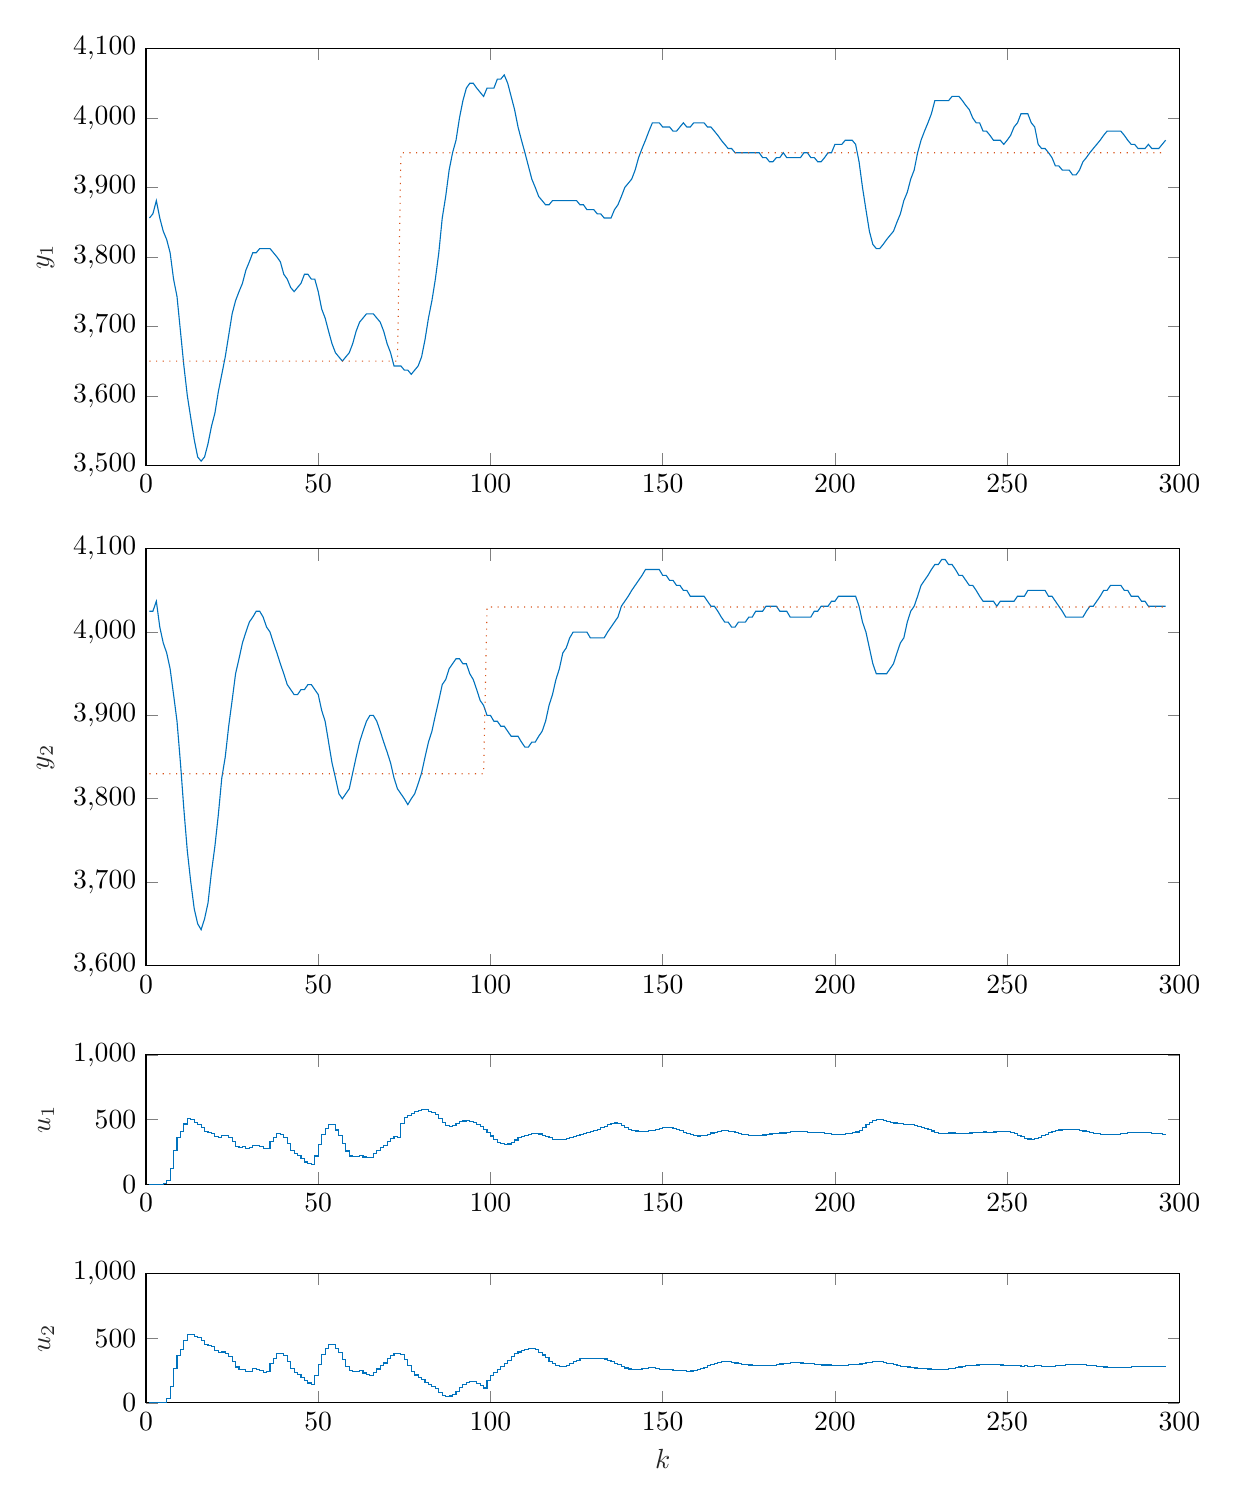
\begin{tikzpicture}

\begin{axis}[%
width=5.167in,
height=0.646in,
at={(0.646in,0.521in)},
scale only axis,
xmin=0,
xmax=300,
xtick={0,50,100,150,200,250,300},
xlabel style={font=\color{white!15!black}},
xlabel={$k$},
ymin=0,
ymax=1000,
ytick={0,500,1000},
ylabel style={font=\color{white!15!black}},
ylabel={$u_2$},
axis background/.style={fill=white}
]
\addplot[const plot, color=mycolor1, forget plot] table[row sep=crcr] {%
1	0\\
2	0\\
3	0\\
4	0\\
5	5\\
6	33\\
7	127\\
8	263\\
9	367\\
10	416\\
11	480\\
12	529\\
13	531\\
14	513\\
15	506\\
16	486\\
17	453\\
18	442\\
19	433\\
20	406\\
21	389\\
22	394\\
23	382\\
24	359\\
25	321\\
26	278\\
27	260\\
28	261\\
29	240\\
30	243\\
31	264\\
32	261\\
33	253\\
34	236\\
35	242\\
36	305\\
37	347\\
38	384\\
39	385\\
40	366\\
41	318\\
42	264\\
43	238\\
44	217\\
45	194\\
46	171\\
47	154\\
48	144\\
49	212\\
50	298\\
51	377\\
52	422\\
53	450\\
54	455\\
55	423\\
56	392\\
57	339\\
58	285\\
59	251\\
60	246\\
61	244\\
62	249\\
63	231\\
64	223\\
65	212\\
66	238\\
67	262\\
68	287\\
69	309\\
70	343\\
71	366\\
72	384\\
73	381\\
74	377\\
75	337\\
76	287\\
77	246\\
78	216\\
79	195\\
80	178\\
81	161\\
82	144\\
83	129\\
84	108\\
85	82\\
86	59\\
87	51\\
88	53\\
89	68\\
90	91\\
91	118\\
92	141\\
93	157\\
94	166\\
95	163\\
96	151\\
97	135\\
98	115\\
99	173\\
100	210\\
101	238\\
102	259\\
103	283\\
104	306\\
105	331\\
106	357\\
107	379\\
108	394\\
109	407\\
110	415\\
111	422\\
112	420\\
113	411\\
114	393\\
115	371\\
116	348\\
117	322\\
118	303\\
119	288\\
120	282\\
121	280\\
122	290\\
123	302\\
124	317\\
125	331\\
126	341\\
127	345\\
128	345\\
129	347\\
130	346\\
131	345\\
132	343\\
133	340\\
134	331\\
135	319\\
136	306\\
137	294\\
138	280\\
139	270\\
140	262\\
141	257\\
142	256\\
143	258\\
144	263\\
145	268\\
146	271\\
147	271\\
148	266\\
149	260\\
150	258\\
151	255\\
152	255\\
153	254\\
154	253\\
155	250\\
156	248\\
157	246\\
158	247\\
159	250\\
160	255\\
161	264\\
162	275\\
163	287\\
164	300\\
165	308\\
166	315\\
167	320\\
168	322\\
169	318\\
170	314\\
171	309\\
172	302\\
173	298\\
174	296\\
175	293\\
176	292\\
177	289\\
178	287\\
179	287\\
180	287\\
181	288\\
182	291\\
183	295\\
184	301\\
185	305\\
186	308\\
187	311\\
188	312\\
189	311\\
190	309\\
191	306\\
192	304\\
193	302\\
194	298\\
195	296\\
196	293\\
197	293\\
198	293\\
199	292\\
200	292\\
201	291\\
202	291\\
203	292\\
204	294\\
205	296\\
206	297\\
207	301\\
208	307\\
209	310\\
210	314\\
211	319\\
212	321\\
213	318\\
214	313\\
215	308\\
216	302\\
217	297\\
218	291\\
219	285\\
220	283\\
221	278\\
222	273\\
223	270\\
224	267\\
225	264\\
226	263\\
227	262\\
228	261\\
229	260\\
230	261\\
231	260\\
232	261\\
233	264\\
234	267\\
235	272\\
236	278\\
237	282\\
238	286\\
239	290\\
240	292\\
241	293\\
242	295\\
243	298\\
244	298\\
245	297\\
246	295\\
247	295\\
248	293\\
249	291\\
250	290\\
251	289\\
252	289\\
253	286\\
254	285\\
255	286\\
256	285\\
257	285\\
258	286\\
259	286\\
260	285\\
261	283\\
262	284\\
263	284\\
264	286\\
265	288\\
266	291\\
267	294\\
268	296\\
269	295\\
270	294\\
271	294\\
272	294\\
273	291\\
274	288\\
275	287\\
276	285\\
277	282\\
278	278\\
279	277\\
280	275\\
281	274\\
282	274\\
283	274\\
284	276\\
285	276\\
286	279\\
287	279\\
288	279\\
289	280\\
290	279\\
291	281\\
292	281\\
293	282\\
294	283\\
295	284\\
296	286\\
};
\end{axis}

\begin{axis}[%
width=5.167in,
height=0.646in,
at={(0.646in,1.615in)},
scale only axis,
xmin=0,
xmax=300,
xtick={0,50,100,150,200,250,300},
ymin=0,
ymax=1000,
ytick={0,500,1000},
ylabel style={font=\color{white!15!black}},
ylabel={$u_1$},
axis background/.style={fill=white}
]
\addplot[const plot, color=mycolor1, forget plot] table[row sep=crcr] {%
1	0\\
2	0\\
3	0\\
4	0\\
5	4\\
6	31\\
7	123\\
8	258\\
9	360\\
10	407\\
11	465\\
12	507\\
13	500\\
14	474\\
15	463\\
16	441\\
17	409\\
18	396\\
19	390\\
20	369\\
21	360\\
22	378\\
23	375\\
24	360\\
25	327\\
26	293\\
27	283\\
28	293\\
29	277\\
30	282\\
31	301\\
32	300\\
33	293\\
34	275\\
35	275\\
36	329\\
37	361\\
38	390\\
39	384\\
40	363\\
41	313\\
42	263\\
43	239\\
44	218\\
45	197\\
46	171\\
47	157\\
48	150\\
49	217\\
50	303\\
51	386\\
52	431\\
53	458\\
54	458\\
55	419\\
56	378\\
57	315\\
58	256\\
59	217\\
60	212\\
61	212\\
62	222\\
63	210\\
64	209\\
65	204\\
66	234\\
67	260\\
68	282\\
69	301\\
70	332\\
71	353\\
72	369\\
73	359\\
74	469\\
75	517\\
76	534\\
77	549\\
78	561\\
79	572\\
80	578\\
81	574\\
82	565\\
83	554\\
84	537\\
85	508\\
86	477\\
87	456\\
88	446\\
89	451\\
90	468\\
91	482\\
92	488\\
93	489\\
94	486\\
95	477\\
96	462\\
97	444\\
98	425\\
99	399\\
100	372\\
101	348\\
102	325\\
103	313\\
104	305\\
105	310\\
106	324\\
107	341\\
108	358\\
109	367\\
110	373\\
111	381\\
112	389\\
113	391\\
114	388\\
115	379\\
116	369\\
117	358\\
118	348\\
119	343\\
120	343\\
121	347\\
122	354\\
123	362\\
124	371\\
125	379\\
126	387\\
127	393\\
128	401\\
129	408\\
130	414\\
131	425\\
132	435\\
133	448\\
134	460\\
135	471\\
136	473\\
137	467\\
138	454\\
139	437\\
140	423\\
141	415\\
142	411\\
143	407\\
144	405\\
145	408\\
146	412\\
147	417\\
148	423\\
149	431\\
150	438\\
151	441\\
152	438\\
153	433\\
154	425\\
155	414\\
156	400\\
157	391\\
158	383\\
159	376\\
160	372\\
161	373\\
162	377\\
163	386\\
164	395\\
165	402\\
166	408\\
167	412\\
168	412\\
169	410\\
170	405\\
171	399\\
172	393\\
173	387\\
174	382\\
175	379\\
176	376\\
177	375\\
178	376\\
179	380\\
180	383\\
181	388\\
182	392\\
183	393\\
184	395\\
185	395\\
186	399\\
187	404\\
188	408\\
189	410\\
190	410\\
191	405\\
192	401\\
193	399\\
194	396\\
195	396\\
196	396\\
197	393\\
198	389\\
199	386\\
200	382\\
201	382\\
202	386\\
203	389\\
204	393\\
205	397\\
206	403\\
207	416\\
208	436\\
209	458\\
210	480\\
211	495\\
212	502\\
213	501\\
214	494\\
215	485\\
216	477\\
217	473\\
218	469\\
219	467\\
220	463\\
221	462\\
222	459\\
223	455\\
224	447\\
225	438\\
226	429\\
227	420\\
228	411\\
229	399\\
230	393\\
231	392\\
232	393\\
233	395\\
234	395\\
235	394\\
236	393\\
237	393\\
238	394\\
239	395\\
240	398\\
241	402\\
242	401\\
243	403\\
244	401\\
245	401\\
246	403\\
247	404\\
248	405\\
249	407\\
250	405\\
251	400\\
252	390\\
253	379\\
254	366\\
255	356\\
256	349\\
257	348\\
258	351\\
259	363\\
260	376\\
261	386\\
262	396\\
263	405\\
264	414\\
265	419\\
266	422\\
267	422\\
268	420\\
269	420\\
270	420\\
271	417\\
272	411\\
273	405\\
274	399\\
275	394\\
276	390\\
277	387\\
278	385\\
279	383\\
280	383\\
281	384\\
282	386\\
283	389\\
284	392\\
285	397\\
286	400\\
287	401\\
288	402\\
289	402\\
290	400\\
291	396\\
292	394\\
293	392\\
294	390\\
295	386\\
296	380\\
};
\end{axis}

\begin{axis}[%
width=5.167in,
height=2.084in,
at={(0.646in,2.708in)},
scale only axis,
xmin=0,
xmax=300,
xtick={0,50,100,150,200,250,300},
ymin=3600,
ymax=4100,
ytick={3600,3700,3800,3900,4000,4100},
ylabel style={font=\color{white!15!black}},
ylabel={$y_2$},
axis background/.style={fill=white}
]
\addplot [color=mycolor1, forget plot]
  table[row sep=crcr]{%
1	4025\\
2	4025\\
3	4037\\
4	4006\\
5	3987\\
6	3975\\
7	3956\\
8	3925\\
9	3893\\
10	3843\\
11	3787\\
12	3737\\
13	3700\\
14	3668\\
15	3650\\
16	3643\\
17	3656\\
18	3675\\
19	3712\\
20	3743\\
21	3781\\
22	3825\\
23	3850\\
24	3887\\
25	3918\\
26	3950\\
27	3968\\
28	3987\\
29	4000\\
30	4012\\
31	4018\\
32	4025\\
33	4025\\
34	4018\\
35	4006\\
36	4000\\
37	3987\\
38	3975\\
39	3962\\
40	3950\\
41	3937\\
42	3931\\
43	3925\\
44	3925\\
45	3931\\
46	3931\\
47	3937\\
48	3937\\
49	3931\\
50	3925\\
51	3906\\
52	3893\\
53	3868\\
54	3843\\
55	3825\\
56	3806\\
57	3800\\
58	3806\\
59	3812\\
60	3831\\
61	3850\\
62	3868\\
63	3881\\
64	3893\\
65	3900\\
66	3900\\
67	3893\\
68	3881\\
69	3868\\
70	3856\\
71	3843\\
72	3825\\
73	3812\\
74	3806\\
75	3800\\
76	3793\\
77	3800\\
78	3806\\
79	3818\\
80	3831\\
81	3850\\
82	3868\\
83	3881\\
84	3900\\
85	3918\\
86	3937\\
87	3943\\
88	3956\\
89	3962\\
90	3968\\
91	3968\\
92	3962\\
93	3962\\
94	3950\\
95	3943\\
96	3931\\
97	3918\\
98	3912\\
99	3900\\
100	3900\\
101	3893\\
102	3893\\
103	3887\\
104	3887\\
105	3881\\
106	3875\\
107	3875\\
108	3875\\
109	3868\\
110	3862\\
111	3862\\
112	3868\\
113	3868\\
114	3875\\
115	3881\\
116	3893\\
117	3912\\
118	3925\\
119	3943\\
120	3956\\
121	3975\\
122	3981\\
123	3993\\
124	4000\\
125	4000\\
126	4000\\
127	4000\\
128	4000\\
129	3993\\
130	3993\\
131	3993\\
132	3993\\
133	3993\\
134	4000\\
135	4006\\
136	4012\\
137	4018\\
138	4031\\
139	4037\\
140	4043\\
141	4050\\
142	4056\\
143	4062\\
144	4068\\
145	4075\\
146	4075\\
147	4075\\
148	4075\\
149	4075\\
150	4068\\
151	4068\\
152	4062\\
153	4062\\
154	4056\\
155	4056\\
156	4050\\
157	4050\\
158	4043\\
159	4043\\
160	4043\\
161	4043\\
162	4043\\
163	4037\\
164	4031\\
165	4031\\
166	4025\\
167	4018\\
168	4012\\
169	4012\\
170	4006\\
171	4006\\
172	4012\\
173	4012\\
174	4012\\
175	4018\\
176	4018\\
177	4025\\
178	4025\\
179	4025\\
180	4031\\
181	4031\\
182	4031\\
183	4031\\
184	4025\\
185	4025\\
186	4025\\
187	4018\\
188	4018\\
189	4018\\
190	4018\\
191	4018\\
192	4018\\
193	4018\\
194	4025\\
195	4025\\
196	4031\\
197	4031\\
198	4031\\
199	4037\\
200	4037\\
201	4043\\
202	4043\\
203	4043\\
204	4043\\
205	4043\\
206	4043\\
207	4031\\
208	4012\\
209	4000\\
210	3981\\
211	3962\\
212	3950\\
213	3950\\
214	3950\\
215	3950\\
216	3956\\
217	3962\\
218	3975\\
219	3987\\
220	3993\\
221	4012\\
222	4025\\
223	4031\\
224	4043\\
225	4056\\
226	4062\\
227	4068\\
228	4075\\
229	4081\\
230	4081\\
231	4087\\
232	4087\\
233	4081\\
234	4081\\
235	4075\\
236	4068\\
237	4068\\
238	4062\\
239	4056\\
240	4056\\
241	4050\\
242	4043\\
243	4037\\
244	4037\\
245	4037\\
246	4037\\
247	4031\\
248	4037\\
249	4037\\
250	4037\\
251	4037\\
252	4037\\
253	4043\\
254	4043\\
255	4043\\
256	4050\\
257	4050\\
258	4050\\
259	4050\\
260	4050\\
261	4050\\
262	4043\\
263	4043\\
264	4037\\
265	4031\\
266	4025\\
267	4018\\
268	4018\\
269	4018\\
270	4018\\
271	4018\\
272	4018\\
273	4025\\
274	4031\\
275	4031\\
276	4037\\
277	4043\\
278	4050\\
279	4050\\
280	4056\\
281	4056\\
282	4056\\
283	4056\\
284	4050\\
285	4050\\
286	4043\\
287	4043\\
288	4043\\
289	4037\\
290	4037\\
291	4031\\
292	4031\\
293	4031\\
294	4031\\
295	4031\\
296	4031\\
};
\addplot [color=mycolor2, dotted, forget plot]
  table[row sep=crcr]{%
1	3830\\
2	3830\\
3	3830\\
4	3830\\
5	3830\\
6	3830\\
7	3830\\
8	3830\\
9	3830\\
10	3830\\
11	3830\\
12	3830\\
13	3830\\
14	3830\\
15	3830\\
16	3830\\
17	3830\\
18	3830\\
19	3830\\
20	3830\\
21	3830\\
22	3830\\
23	3830\\
24	3830\\
25	3830\\
26	3830\\
27	3830\\
28	3830\\
29	3830\\
30	3830\\
31	3830\\
32	3830\\
33	3830\\
34	3830\\
35	3830\\
36	3830\\
37	3830\\
38	3830\\
39	3830\\
40	3830\\
41	3830\\
42	3830\\
43	3830\\
44	3830\\
45	3830\\
46	3830\\
47	3830\\
48	3830\\
49	3830\\
50	3830\\
51	3830\\
52	3830\\
53	3830\\
54	3830\\
55	3830\\
56	3830\\
57	3830\\
58	3830\\
59	3830\\
60	3830\\
61	3830\\
62	3830\\
63	3830\\
64	3830\\
65	3830\\
66	3830\\
67	3830\\
68	3830\\
69	3830\\
70	3830\\
71	3830\\
72	3830\\
73	3830\\
74	3830\\
75	3830\\
76	3830\\
77	3830\\
78	3830\\
79	3830\\
80	3830\\
81	3830\\
82	3830\\
83	3830\\
84	3830\\
85	3830\\
86	3830\\
87	3830\\
88	3830\\
89	3830\\
90	3830\\
91	3830\\
92	3830\\
93	3830\\
94	3830\\
95	3830\\
96	3830\\
97	3830\\
98	3830\\
99	4030\\
100	4030\\
101	4030\\
102	4030\\
103	4030\\
104	4030\\
105	4030\\
106	4030\\
107	4030\\
108	4030\\
109	4030\\
110	4030\\
111	4030\\
112	4030\\
113	4030\\
114	4030\\
115	4030\\
116	4030\\
117	4030\\
118	4030\\
119	4030\\
120	4030\\
121	4030\\
122	4030\\
123	4030\\
124	4030\\
125	4030\\
126	4030\\
127	4030\\
128	4030\\
129	4030\\
130	4030\\
131	4030\\
132	4030\\
133	4030\\
134	4030\\
135	4030\\
136	4030\\
137	4030\\
138	4030\\
139	4030\\
140	4030\\
141	4030\\
142	4030\\
143	4030\\
144	4030\\
145	4030\\
146	4030\\
147	4030\\
148	4030\\
149	4030\\
150	4030\\
151	4030\\
152	4030\\
153	4030\\
154	4030\\
155	4030\\
156	4030\\
157	4030\\
158	4030\\
159	4030\\
160	4030\\
161	4030\\
162	4030\\
163	4030\\
164	4030\\
165	4030\\
166	4030\\
167	4030\\
168	4030\\
169	4030\\
170	4030\\
171	4030\\
172	4030\\
173	4030\\
174	4030\\
175	4030\\
176	4030\\
177	4030\\
178	4030\\
179	4030\\
180	4030\\
181	4030\\
182	4030\\
183	4030\\
184	4030\\
185	4030\\
186	4030\\
187	4030\\
188	4030\\
189	4030\\
190	4030\\
191	4030\\
192	4030\\
193	4030\\
194	4030\\
195	4030\\
196	4030\\
197	4030\\
198	4030\\
199	4030\\
200	4030\\
201	4030\\
202	4030\\
203	4030\\
204	4030\\
205	4030\\
206	4030\\
207	4030\\
208	4030\\
209	4030\\
210	4030\\
211	4030\\
212	4030\\
213	4030\\
214	4030\\
215	4030\\
216	4030\\
217	4030\\
218	4030\\
219	4030\\
220	4030\\
221	4030\\
222	4030\\
223	4030\\
224	4030\\
225	4030\\
226	4030\\
227	4030\\
228	4030\\
229	4030\\
230	4030\\
231	4030\\
232	4030\\
233	4030\\
234	4030\\
235	4030\\
236	4030\\
237	4030\\
238	4030\\
239	4030\\
240	4030\\
241	4030\\
242	4030\\
243	4030\\
244	4030\\
245	4030\\
246	4030\\
247	4030\\
248	4030\\
249	4030\\
250	4030\\
251	4030\\
252	4030\\
253	4030\\
254	4030\\
255	4030\\
256	4030\\
257	4030\\
258	4030\\
259	4030\\
260	4030\\
261	4030\\
262	4030\\
263	4030\\
264	4030\\
265	4030\\
266	4030\\
267	4030\\
268	4030\\
269	4030\\
270	4030\\
271	4030\\
272	4030\\
273	4030\\
274	4030\\
275	4030\\
276	4030\\
277	4030\\
278	4030\\
279	4030\\
280	4030\\
281	4030\\
282	4030\\
283	4030\\
284	4030\\
285	4030\\
286	4030\\
287	4030\\
288	4030\\
289	4030\\
290	4030\\
291	4030\\
292	4030\\
293	4030\\
294	4030\\
295	4030\\
296	4030\\
};
\end{axis}

\begin{axis}[%
width=5.167in,
height=2.084in,
at={(0.646in,5.209in)},
scale only axis,
xmin=0,
xmax=300,
xtick={0,50,100,150,200,250,300},
ymin=3500,
ymax=4100,
ytick={3500,3600,3700,3800,3900,4000,4100},
ylabel style={font=\color{white!15!black}},
ylabel={$y_1$},
axis background/.style={fill=white}
]
\addplot [color=mycolor1, forget plot]
  table[row sep=crcr]{%
1	3856\\
2	3862\\
3	3881\\
4	3856\\
5	3837\\
6	3825\\
7	3806\\
8	3768\\
9	3743\\
10	3693\\
11	3643\\
12	3600\\
13	3568\\
14	3537\\
15	3512\\
16	3506\\
17	3512\\
18	3531\\
19	3556\\
20	3575\\
21	3606\\
22	3631\\
23	3656\\
24	3687\\
25	3718\\
26	3737\\
27	3750\\
28	3762\\
29	3781\\
30	3793\\
31	3806\\
32	3806\\
33	3812\\
34	3812\\
35	3812\\
36	3812\\
37	3806\\
38	3800\\
39	3793\\
40	3775\\
41	3768\\
42	3756\\
43	3750\\
44	3756\\
45	3762\\
46	3775\\
47	3775\\
48	3768\\
49	3768\\
50	3750\\
51	3725\\
52	3712\\
53	3693\\
54	3675\\
55	3662\\
56	3656\\
57	3650\\
58	3656\\
59	3662\\
60	3675\\
61	3693\\
62	3706\\
63	3712\\
64	3718\\
65	3718\\
66	3718\\
67	3712\\
68	3706\\
69	3693\\
70	3675\\
71	3662\\
72	3643\\
73	3643\\
74	3643\\
75	3637\\
76	3637\\
77	3631\\
78	3637\\
79	3643\\
80	3656\\
81	3681\\
82	3712\\
83	3737\\
84	3768\\
85	3806\\
86	3856\\
87	3887\\
88	3925\\
89	3950\\
90	3968\\
91	4000\\
92	4025\\
93	4043\\
94	4050\\
95	4050\\
96	4043\\
97	4037\\
98	4031\\
99	4043\\
100	4043\\
101	4043\\
102	4056\\
103	4056\\
104	4062\\
105	4050\\
106	4031\\
107	4012\\
108	3987\\
109	3968\\
110	3950\\
111	3931\\
112	3912\\
113	3900\\
114	3887\\
115	3881\\
116	3875\\
117	3875\\
118	3881\\
119	3881\\
120	3881\\
121	3881\\
122	3881\\
123	3881\\
124	3881\\
125	3881\\
126	3875\\
127	3875\\
128	3868\\
129	3868\\
130	3868\\
131	3862\\
132	3862\\
133	3856\\
134	3856\\
135	3856\\
136	3868\\
137	3875\\
138	3887\\
139	3900\\
140	3906\\
141	3912\\
142	3925\\
143	3943\\
144	3956\\
145	3968\\
146	3981\\
147	3993\\
148	3993\\
149	3993\\
150	3987\\
151	3987\\
152	3987\\
153	3981\\
154	3981\\
155	3987\\
156	3993\\
157	3987\\
158	3987\\
159	3993\\
160	3993\\
161	3993\\
162	3993\\
163	3987\\
164	3987\\
165	3981\\
166	3975\\
167	3968\\
168	3962\\
169	3956\\
170	3956\\
171	3950\\
172	3950\\
173	3950\\
174	3950\\
175	3950\\
176	3950\\
177	3950\\
178	3950\\
179	3943\\
180	3943\\
181	3937\\
182	3937\\
183	3943\\
184	3943\\
185	3950\\
186	3943\\
187	3943\\
188	3943\\
189	3943\\
190	3943\\
191	3950\\
192	3950\\
193	3943\\
194	3943\\
195	3937\\
196	3937\\
197	3943\\
198	3950\\
199	3950\\
200	3962\\
201	3962\\
202	3962\\
203	3968\\
204	3968\\
205	3968\\
206	3962\\
207	3937\\
208	3900\\
209	3868\\
210	3837\\
211	3818\\
212	3812\\
213	3812\\
214	3818\\
215	3825\\
216	3831\\
217	3837\\
218	3850\\
219	3862\\
220	3881\\
221	3893\\
222	3912\\
223	3925\\
224	3950\\
225	3968\\
226	3981\\
227	3993\\
228	4006\\
229	4025\\
230	4025\\
231	4025\\
232	4025\\
233	4025\\
234	4031\\
235	4031\\
236	4031\\
237	4025\\
238	4018\\
239	4012\\
240	4000\\
241	3993\\
242	3993\\
243	3981\\
244	3981\\
245	3975\\
246	3968\\
247	3968\\
248	3968\\
249	3962\\
250	3968\\
251	3975\\
252	3987\\
253	3993\\
254	4006\\
255	4006\\
256	4006\\
257	3993\\
258	3987\\
259	3962\\
260	3956\\
261	3956\\
262	3950\\
263	3943\\
264	3931\\
265	3931\\
266	3925\\
267	3925\\
268	3925\\
269	3918\\
270	3918\\
271	3925\\
272	3937\\
273	3943\\
274	3950\\
275	3956\\
276	3962\\
277	3968\\
278	3975\\
279	3981\\
280	3981\\
281	3981\\
282	3981\\
283	3981\\
284	3975\\
285	3968\\
286	3962\\
287	3962\\
288	3956\\
289	3956\\
290	3956\\
291	3962\\
292	3956\\
293	3956\\
294	3956\\
295	3962\\
296	3968\\
};
\addplot [color=mycolor2, dotted, forget plot]
  table[row sep=crcr]{%
1	3650\\
2	3650\\
3	3650\\
4	3650\\
5	3650\\
6	3650\\
7	3650\\
8	3650\\
9	3650\\
10	3650\\
11	3650\\
12	3650\\
13	3650\\
14	3650\\
15	3650\\
16	3650\\
17	3650\\
18	3650\\
19	3650\\
20	3650\\
21	3650\\
22	3650\\
23	3650\\
24	3650\\
25	3650\\
26	3650\\
27	3650\\
28	3650\\
29	3650\\
30	3650\\
31	3650\\
32	3650\\
33	3650\\
34	3650\\
35	3650\\
36	3650\\
37	3650\\
38	3650\\
39	3650\\
40	3650\\
41	3650\\
42	3650\\
43	3650\\
44	3650\\
45	3650\\
46	3650\\
47	3650\\
48	3650\\
49	3650\\
50	3650\\
51	3650\\
52	3650\\
53	3650\\
54	3650\\
55	3650\\
56	3650\\
57	3650\\
58	3650\\
59	3650\\
60	3650\\
61	3650\\
62	3650\\
63	3650\\
64	3650\\
65	3650\\
66	3650\\
67	3650\\
68	3650\\
69	3650\\
70	3650\\
71	3650\\
72	3650\\
73	3650\\
74	3950\\
75	3950\\
76	3950\\
77	3950\\
78	3950\\
79	3950\\
80	3950\\
81	3950\\
82	3950\\
83	3950\\
84	3950\\
85	3950\\
86	3950\\
87	3950\\
88	3950\\
89	3950\\
90	3950\\
91	3950\\
92	3950\\
93	3950\\
94	3950\\
95	3950\\
96	3950\\
97	3950\\
98	3950\\
99	3950\\
100	3950\\
101	3950\\
102	3950\\
103	3950\\
104	3950\\
105	3950\\
106	3950\\
107	3950\\
108	3950\\
109	3950\\
110	3950\\
111	3950\\
112	3950\\
113	3950\\
114	3950\\
115	3950\\
116	3950\\
117	3950\\
118	3950\\
119	3950\\
120	3950\\
121	3950\\
122	3950\\
123	3950\\
124	3950\\
125	3950\\
126	3950\\
127	3950\\
128	3950\\
129	3950\\
130	3950\\
131	3950\\
132	3950\\
133	3950\\
134	3950\\
135	3950\\
136	3950\\
137	3950\\
138	3950\\
139	3950\\
140	3950\\
141	3950\\
142	3950\\
143	3950\\
144	3950\\
145	3950\\
146	3950\\
147	3950\\
148	3950\\
149	3950\\
150	3950\\
151	3950\\
152	3950\\
153	3950\\
154	3950\\
155	3950\\
156	3950\\
157	3950\\
158	3950\\
159	3950\\
160	3950\\
161	3950\\
162	3950\\
163	3950\\
164	3950\\
165	3950\\
166	3950\\
167	3950\\
168	3950\\
169	3950\\
170	3950\\
171	3950\\
172	3950\\
173	3950\\
174	3950\\
175	3950\\
176	3950\\
177	3950\\
178	3950\\
179	3950\\
180	3950\\
181	3950\\
182	3950\\
183	3950\\
184	3950\\
185	3950\\
186	3950\\
187	3950\\
188	3950\\
189	3950\\
190	3950\\
191	3950\\
192	3950\\
193	3950\\
194	3950\\
195	3950\\
196	3950\\
197	3950\\
198	3950\\
199	3950\\
200	3950\\
201	3950\\
202	3950\\
203	3950\\
204	3950\\
205	3950\\
206	3950\\
207	3950\\
208	3950\\
209	3950\\
210	3950\\
211	3950\\
212	3950\\
213	3950\\
214	3950\\
215	3950\\
216	3950\\
217	3950\\
218	3950\\
219	3950\\
220	3950\\
221	3950\\
222	3950\\
223	3950\\
224	3950\\
225	3950\\
226	3950\\
227	3950\\
228	3950\\
229	3950\\
230	3950\\
231	3950\\
232	3950\\
233	3950\\
234	3950\\
235	3950\\
236	3950\\
237	3950\\
238	3950\\
239	3950\\
240	3950\\
241	3950\\
242	3950\\
243	3950\\
244	3950\\
245	3950\\
246	3950\\
247	3950\\
248	3950\\
249	3950\\
250	3950\\
251	3950\\
252	3950\\
253	3950\\
254	3950\\
255	3950\\
256	3950\\
257	3950\\
258	3950\\
259	3950\\
260	3950\\
261	3950\\
262	3950\\
263	3950\\
264	3950\\
265	3950\\
266	3950\\
267	3950\\
268	3950\\
269	3950\\
270	3950\\
271	3950\\
272	3950\\
273	3950\\
274	3950\\
275	3950\\
276	3950\\
277	3950\\
278	3950\\
279	3950\\
280	3950\\
281	3950\\
282	3950\\
283	3950\\
284	3950\\
285	3950\\
286	3950\\
287	3950\\
288	3950\\
289	3950\\
290	3950\\
291	3950\\
292	3950\\
293	3950\\
294	3950\\
295	3950\\
296	3950\\
};
\end{axis}
\end{tikzpicture}%
\caption{Przebieg dla regulatora DMC o $\lambda = 5$ oraz $N = N_\mathrm{u} = D = 80$.}
\label{Z4DMCfinal}
\end{figure}

\chapter{Podpunkt 5}
Wyświetlane na panelu wartości prezentowane są w prostej formie słupków z podanymi przy nich wartościami numerycznymi. Ponieważ element wyświetlający wartości numeryczne może także działać jako wejście umożliwiliśmy zadawanie w ten sposób wartości zadanej (uwaga --- wymaga to wykomentowania ustawionej w kodzie trajektorii tak aby jedno nie kłóciło się z drugim). Poniżej zamieszczono zdjęcie panelu podczas pracy. Projekt panelu znajduje się w pliku \verb+simple_GOT.GTX+.

\begin{figure}[ht]
\centering
\includegraphics[width=\textwidth]{im/6.jpg}
\caption{Zdjęcie panelu podczas pracy.}
\end{figure}

\chapter{Podpunkt 6}
Pracę nad automatem stanów rozpoczęto od podania wartości zadanych w instrukcjach warunkowych umożliwiając uzyskanie czterech stanów poprzez kombinacje niskich i wysokich wartości zadanych na każdym z wyjść. Niestety ze względu na ograniczenia czasowe po konsultacji z prowadzącym dostaliśmy polecenie przejścia do kolejnych podpunktów, stąd implementacja nie została dokończona.

\chapter{Podpunkt 7}
Zastosowana konfiguracja wymagała przede wszystkich włączenia czterech kanałów PWM --- Y0 to sygnał sterujący silnikiem ze stałą częstotliwością 10kHz, zaś kanały Y1-Y3 sterują zaworami. Niestety dla wypełnień sygnału pompy poniżej 40\% układ nie był w stanie pokonać grawitacji, przy wyższych wypełnieniach niestety zawory nie były w stanie opróżniać zbiorników szybciej niż te były wypełniane przez pompę. Stąd układ okazał się dużo bardziej problematyczny niż pierwotnie zakładano, w końcowej wersji zawory manualne zostały w pełni otwarte, a wypełnienie pompy ustawione na 60\%. Sterowanie odbywa się poprzez zmianę wypełnienia zaworów.

Poza kanałami PWM włączone zostały także trzy kanały ``High Speed I/O'' mieżące sygnał częstotliwościowy pomiaru wysokości cieczy w zbiornikach.

\chapter{Podpunkty 8 i 9}
Implementacja zabezpieczenia stanowiska przed uszkodzeniem początkowo opierała się o intrukcję warunkową wyłączającą pompę i otwierającą zawory w razie osiągnięcia niebezpiecznego poziomu wody, jednkaże w czasie pracy okazało się, że nie była ona potrzebna ze względu na prędkość pompowania wody, nawet przy zamkniętych zaworach obecne w stanowisku odpływy w pełni radziły sobie z zapobiegnięciem przekroczenia bezpiecznego poziomu wody. Stąd zastosowane podejście opierało się o sprawdzenie i potwierdzenie sprawności istniejącego już mechanizmu.

Ze względu na problemy ze skonfigurowaniem stanowiska i początkowe problemy z działaniem pompy (przy wypełnieniu 40\%) w ograniczonym czasie nie udało się nam wyznaczyć charakterystyki statycznej. Jednakże nawet bez charakterystyki statycznej ze względu na strukturę stanowiska łatwo zauważyć, że dla każdego z wyjść (poziom wody w zbiorniku) największy wpływ na nie ma wejście będące sterowaniem zaworu opróźniającego dany zbiornik.

\chapter{Podpunkt 10}
Dostosowanie implementacji regulatora PID do obiektu Inteco opierało się przede wszystkim o dodanie trzeciego regulatora, zmianę wejść na odpowiednie rejestry oraz zmianę sposobu zadawania wyjścia na sterowanie wypełnieniem sygnału PWM. Ograniczenia zostały uwzględnione poprzez odpowiednie przycięcie sygnałów sterujących do zakresu 1-100\%. Wynika to z faktu, że zerowe wypełnienie nie jest akceptowane i wywołuje błąd.

Planowane było dobieranie nastaw osobno dla każdego z regulatorów zaczynając od górnego zbiornika, niestety mimo poświęcenia na dobór parametrów ponad godziny czasu nie udało się nam dobrać parametrów nawet dla pierwszego z regulatorów.

\chapter{Podpunkty 11 i 12}
Ze względu na ograniczenia czasowe i charakter stanowiska po konsultacji z prowadzącym uzgodniono, że podpunkty te nie będą wykonywane.

\chapter{Podpunkt 13}
Przygotowana wizualizacja procesu pokazuje w prostej formie graficznej schemat stanowiska w formie odpowiednio wypełniających się zbiorników. Obok zbiorników wizualizowana jest wartość zadana dla każdego ze zbiorników (może być zadawana z poziomu panelu), a poza tym dla każdej z istotnych wartości wyświetlana jest jej wartość numeryczna. Podjęta została próba dokładnego odwzorowania zbiorników (prostokąt, ścięty trójkąt, wycinek koła), ale niestety mimo długiej konsultacji z prowadzącym nie udało nam się tego dokonać w dostępnym oprogramowaniu, stąd też wszystkie zbiorniki widoczne są jako prostokąty. Poniżej przedstawiono zdjęcie panelu.

\begin{figure}[ht]
\centering
\includegraphics[width=\textwidth]{im/2.jpg}
\caption{Zdjęcie panelu dla obiektu Inteco.}
\end{figure}

